%%%%%%%%%%%%%%%%%%%%%%%%%%%%%%%%%%%%%%%%%%%%%%%%%%%%%%%%%%%%%%%%%%%%%%%%%%%%%%%%%%%%%%%%%
% Template de l'elaboració de TFG del Grau en informàtica de la Universitat de Girona (udg.)
% basat en https://github.com/matteodelucchi/ZHAW_thesis-template
%
% This template is based on previous works by:
% Steve Gunn (http://users.ecs.soton.ac.uk/srg/softwaretools/document/templates/)
% Sunil Patel (http://www.sunilpatel.co.uk/thesis-template/)
% Matteo Delucchi (https://github.com/matteodelucchi/ZHAW_thesis-template)
%
% University specific changes were made by:
%  Robert Martí (robert.marti@udg.edu)
% 
% Template license:
% CC BY-NC-SA 3.0 (http://creativecommons.org/licenses/by-nc-sa/3.0/)
%%%%%%%%%%%%%%%%%%%%%%%%%%%%%%%%%%%%%%%%%%%%%%%%%%%%%%%%%%%%%%%%%%%%%%%%%%%%%%%%%%%%%%%%%

%----------------------------------------------------------------------------------------
% DOCUMENT SPECIFICATION
%----------------------------------------------------------------------------------------
\documentclass[
    11pt,                      % Default font size
    %oneside,                  % One-side binding. Default: Two-side binding / alternating margins
    catalan,                   % Language. Feu servir english per anglès
    singlespacing,             % Spacing option: singlespacing, onehalfspacing or doublespacing
    %nolistspacing,            % Set spacing in lists to single
    %draft,                    % Enable draft mode: no pictures, no links, overfull hboxes indicated
    liststotoc,               % Include list of figures/tables/etc in the table of contents
    %toctotoc,                 % Include the main table of contents to the table of contents
    parskip,                  % Add vertical space between paragraphs
    %nohyperref,               % Disable links in the entire document
    headsepline,               % Show a horizontal line under the header
    %chapterinoneline,         % Place the chapter title and chapter number on one line
    consistentlayout,          % Have the same layout for special chapters: 
                               % declaration, abstract and acknowledgements
]{MastersDoctoralThesis}

% Uncomment the following lines to only include a subset of chapters.
% This is useful for long documents, as typesetting takes a bit of time
%\includeonly{
%    Front/titlepage,
%    Front/imprint,
%    Front/abstract,
%    %Front/declaration,
%    %Front/acknowledgements,
%    %Front/symbols,
%    Chapters/Chapter1,
%    %Chapters/Chapter2
%    }


%----------------------------------------------------------------------------------------
% PREAMBLE: PACKAGES AND CONFIGURATIONS
%----------------------------------------------------------------------------------------
% !TEX root = main.tex

%----------------------------
%   Fonts and characters
%----------------------------

% Support for special characters
\usepackage[utf8]{inputenc}    % Specify input encoding
\usepackage[T1]{fontenc}       % Specify font encoding

% Set main fonts
% Fonts catalogue: https://tug.org/FontCatalogue/
\usepackage{mathpazo}          % Use the Palatino font by default
\usepackage{beramono}          % Override the monospace/typewriter font

% UdG title font
% Try to load Georgia 
% Loading OTF or system fonts is possible with XeLaTeX.
% If the document is compiled using pdfLaTeX, resort 
\usepackage{ifxetex}
\ifxetex
    \usepackage{fontspec}
    \newfontfamily\udgtitlefont{Georgia}
\else
    \newcommand{\zhawtitlefont}{\scshape}
\fi

%\usepackage[scaled]{helvet}

%----------------------------
%   Environments
%----------------------------

\usepackage{caption}           % Customized caption
\usepackage{subcaption}        % Subfigure captions
\usepackage{makecell}          % Per-cell formatting in tables (\makecell)
\usepackage{pdfpages}          % Required to include PDF files/graphics (\includepdf)

\usepackage{todonotes}         % Introduces the command \todo
\setlength{\marginparwidth}{2.5cm} % Adjust this if the todo notes are out of margins

% Create boxes as follows:
% \begin{colorbox}{red}{2}
\usepackage{tcolorbox}
\newtcolorbox{textbox}[2]{
    arc=3pt,
    boxrule=#2pt,
    colback=#1!25!white,
    width=\textwidth,
    halign=left,
    valign=center,
    colframe=#1!75!black
}

%----------------------------
%   Colors
%----------------------------

% Set up colors
\usepackage{xcolor}
% UdG Blue: Pantone 2945 U / R0 G20 B137
\definecolor{udgblue}{rgb}{0.00, 0.07, 0.54}
% Colors related to code listings
\definecolor{codegreen}{rgb}{0,0.6,0}
\definecolor{codegray}{rgb}{0.5,0.5,0.5}
\definecolor{codepurple}{rgb}{0.58,0,0.82}
\definecolor{codebackground}{rgb}{0.93,0.94,0.95}

%----------------------------
%   Code listings
%----------------------------

% Setup code listings
\usepackage{listings}
\lstdefinestyle{mystyle}{
    backgroundcolor=\color{codebackground},   
    commentstyle=\color{codegreen},
    keywordstyle=\color{magenta},
    numberstyle=\tiny\color{codegray},
    stringstyle=\color{codepurple},
    basicstyle=\ttfamily\footnotesize,
    breakatwhitespace=false,
    breaklines=true,
%    captionpos=b,
    keepspaces=true,
    numbers=left,
    numbersep=5pt,
    showspaces=false,
    showstringspaces=false,
    showtabs=false,
    tabsize=4
}
\lstset{style=mystyle}

% minted is an alternative code listing package. (See chapter 2)
% For it to run successfully, ensure the following:
% - the Python package Pygments. Install with the following command:
%       python -m pip install Pygments
% - pdflatex (or xelatex) is executed with the flag --shell-escape
%   If you are using a TEX editor, you can modify the typesetting 
%   command somewhere in the settings.
%\usepackage[outputdir=build]{minted}
%\usemintedstyle{xcode}
% For fancier coloring schemes, see here:
% https://tex.stackexchange.com/questions/585582
% One could also create an own style in Pygments
% https://pygments.org/docs/styles/#creating-own-styles

%----------------------------
%   References
%----------------------------

% Set up references
\usepackage[
    backend=biber,             % Use biber backend (an external tool)
    sorting=none,              % Enumerates the reference in order of their appearance
    style=numeric-comp         % Choose here your preferred citation style
]{biblatex}
\addbibresource{example.bib}   % The filename of the bibliography
\usepackage[autostyle=false]{csquotes} 
                               % Required to generate language-dependent quotes 
                               % in the bibliography

%----------------------------------------------------------------------------------------
%   MARGIN SETTINGS
%----------------------------------------------------------------------------------------

\geometry{
    paper=a4paper,      % Change to letterpaper for US letter
    inner=2.5cm,        % Inner margin
    outer=3.8cm,        % Outer margin
    top=1.5cm,          % Top margin
    bottom=1.5cm,       % Bottom margin
    bindingoffset=.5cm, % Binding offset
    %showframe,         % Show the type block of the page
}
\setlength{\parskip}{1em}
\usepackage{enumitem}          % Layout control for list environments (e.g, itemize)
%\setlist{noitemsep}           % Suppress extra spaces between items
%\setlist{nosep}               % Suppress spaces before/after list environments

\usepackage{rotating}
\usepackage{amsmath}
\usepackage{float}
\usepackage{graphicx}
\usepackage{caption}
\usepackage{subcaption}
\usepackage{enumitem}
\usepackage{pgf-umlcd}
\usepackage{pgfplots}

\renewcommand{\umltextcolor}{black}
\renewcommand{\umldrawcolor}{black}
\renewcommand{\umlfillcolor}{white}
\pgfplotsset{width=10cm,compat=1.9}
%----------------------------------------------------------------------------------------
% THESIS INFORMATION: MODIFY THIS SECTION!
%----------------------------------------------------------------------------------------

% The information below is used in the following parts:
% - Title page
% - Imprint
% - Abstract / Zusammenfassung
% - Meta information of PDF

\thesistitle{Factorio Planner}             % Thesis title,              command: \ttitle
\thesistype{Projecte Final de Grau}             % Type of thesis (e.g. Master Thesis) \ttype
\thesisdocument{Memòria}
\thesisdate{Setembre 2024}                     % Date of submission                  \tdate
\keywords{gravity, physics, disruptive science}
                                        % Keywords for the thesis,            \keywordnames
\author{Pau Jimeno Román}             % Your name,                          \authorname
\degree{Grau en Enginyeria Informàtica} % Degree name,                        \degreename
\studyprogram{Grau en Enginyeria Informàtica} 
                                        % Study program                       \studyprog
% \studyprogramlink{https://www.zhaw.ch/en/lsfm/study/master/applied-computational-life-sciences/}
                                        % Link to study program               \studyproglink

\supervisorA{Dr. Mateu Villaret Auselle}       % Name of supervisor 1,               \supnameA
\supervisorAmail{mvillaret@udg.edu}         % Email address of supervisor 1,      \supmailA
\supervisorAweb{https://www.udg.edu/ca/directori/pagina-personal?ID=52807}  %            \supwebA
\supervisorAinfo{                       % Formatted info about supervisor 1:  \supinfoA
    \supnameA\\
    Universitat de Girona\\
    Email: \href{mailto:\supmailA}{\supmailA}\\
    Web: \href{\supwebA}{Perfil UdG}
}

% Keep empty if there is no supervisor 2: \supervisorB{}
\supervisorB{}              % Name of supervisor 2,               \supnameB
\supervisorBmail{f=am@newton.com}       % Email address of supervisor 2,      \supmailB
\supervisorBweb{https://ca.wikipedia.org/wiki/Isaac_Newton}                  % \supwebB
\supervisorBinfo{                       % Formatted info about supervisor 2:  \supinfoB
    \supnameB\\
    University of Cambridge\\
    Email: \href{mailto:\supmailB}{\supmailB}\\
    Web: \href{\supwebB}{Link}
}

\university{University of Girona}
                                        % University name                     \univname
\universitycatalan{Universitat de Girona}
                                        % University, in German               \univnameger
\department{Arquitectura i Tecnologia de computadors} 
                                        % Department,                         \deptname

% % Links
\universitylink      {https://www.udg.edu/}                   % \univlink
% \universitylinkgerman{https://www.zhaw.ch/de/university/}                   % \univlinkger
% \departmentlink      {https://www.zhaw.ch/de/lsfm/}                         % \deptlink
% \institutelink       {https://www.zhaw.ch/en/lsfm/institutes-centres/icls/} % \instlink
% \grouplink           {https://www.zhaw.ch/en/lsfm/institutes-centres/icls/computational-health/} % \grplink



\AtBeginDocument{
\hypersetup{pdftitle=\ttitle} % Set the PDF's title to your title
\hypersetup{pdfauthor=\authorname} % Set the PDF's author to your name
\hypersetup{pdfkeywords=\keywordnames} % Set the PDF's keywords to your keywords
}

\begin{document}
\frontmatter                  % Roman page numbering for the pre-content pages
\pagestyle{plain}             % Default to the plain heading style until the thesis style 
                              % is called for the body content


%----------------------------------------------------------------------------------------
% TITLE PAGE AND IMPRINT
%----------------------------------------------------------------------------------------
% !TEX root = ../main.tex

%----------------------------------------------------------------------------------------
% TITLE PAGE
%----------------------------------------------------------------------------------------

\newgeometry{margin=1in}
\begin{titlepage}

% Make the title page mostly inert to the parskip-setting.
\setlength{\parskip}{0pt}

\begin{center}

\includegraphics[width=0.65\textwidth]{Figures/EPS_centrat.png}

\vspace{2cm}

{\Large \studyprog\par}                      % Estudi
\vspace{0.2cm}
\vspace{3.5cm}                            
\textsc{\Large \ttype}                                 % Thesis type
\vspace{0.2cm}

\HRule 
\vspace{0.4cm}
{\huge \bfseries \ttitle\par}                          % Thesis title
\vspace{0.4cm}  
\HRule
\vspace{1cm}
 
\begin{minipage}[t]{0.4\textwidth}
\begin{flushleft} 
    \large
    \emph{Autor:}\\
    \authorname
\end{flushleft}
\end{minipage}
\begin{minipage}[t]{0.4\textwidth}
\begin{flushright} 
    \large
    \emph{Tutor:} \\
    \supnameA \\
    \supnameB
\end{flushright}
\end{minipage}

\vspace{2.5cm}
 \textsc{\Large \tdocument}                                 % Thesis type
\vspace{0.2cm}

\vfill

{\large
Convocatòria:\\                                %Convodatòria
\tdate\\
\vspace{1.5cm}
Departament :\\
\deptname\\                                    %Departament
}
\vfill
\end{center}
\end{titlepage}
\restoregeometry

\let\cleardoublepage\clearpage
% !TEX root = ../main.tex

%----------------------------------------------------------------------------------------
% IMPRINT
%----------------------------------------------------------------------------------------

\thispagestyle{empty}
\vspace*{\fill}

{\bfseries  \Large }
\vspace{0.75cm}

\begin{footnotesize}


\begin{flushleft} 
\begin{tabular}{ @{}lp{0.6\textwidth}@{} } 
\emph{Projecte:}  & \ttype\\ 
\emph{Document:}  & \tdocument\\ 
\emph{Títol}:    & \ttitle\\
\emph{Autor}:   & \authorname\\
\emph{Data}:     & \tdate\\
% \emph{Copyright}:& \univname

\end{tabular}
\end{flushleft}

\vspace{0.75cm}


\begin{minipage}[t]{0.95\textwidth}
\begin{flushleft} 
\emph{Estudi:}\\
%\href{\studyproglink}{\studyprog}\\
\studyprog\\
\href{\univlink}{\univnamecat}
\end{flushleft}
\end{minipage}

\vspace{0.75cm}

\begin{minipage}[t]{0.50\textwidth}
\begin{flushleft} 
\emph{Supervisor:}\\
\supinfoA
\end{flushleft}
\end{minipage}
\begin{minipage}[t]{0.45\textwidth}
\begin{flushleft} 
\ifdefempty{\supnameB}
{}
{
    \emph{Supervisor 2:}\\
    \supinfoB
}
\end{flushleft}
\end{minipage}

\end{footnotesize}





%----------------------------------------------------------------------------------------
% ABSTRACT
%----------------------------------------------------------------------------------------
%% !TEX root = ../main.tex

%----------------------------------------------------------------------------------------
% ABSTRACT PAGE
%----------------------------------------------------------------------------------------
\begin{abstract}
\addchaptertocentry{\abstractname} % Add the abstract to the table of contents
The abstract is like a miniature version of the entire manuscript. Structure it similarly: Begin with the context and motivation for the project, a brief description of the method and available data, your findings, and conclusions. Limit yourself to one page!
\end{abstract}





%----------------------------------------------------------------------------------------
% ACKNOWLEDGEMENTS
%----------------------------------------------------------------------------------------
%% !TEX root = ../main.tex

%----------------------------------------------------------------------------------------
% ACKNOWLEDGEMENTS
%----------------------------------------------------------------------------------------
\begin{acknowledgements}
\addchaptertocentry{\acknowledgementname} % Add the acknowledgements to the table of contents

The acknowledgements belong here. Do not forget to mention your project supervisors, without flattering them too much.
\end{acknowledgements}



%----------------------------------------------------------------------------------------
% LIST OF CONTENTS/FIGURES/TABLES PAGES
%----------------------------------------------------------------------------------------
% Comment out if any of the following is not needed:
\tableofcontents  % Add main table of contents
%\listoffigures    % Add list of figures
%\listoftables     % Add list of tables


%----------------------------------------------------------------------------------------
% ABBREVIATIONS / SYMBOLS
%----------------------------------------------------------------------------------------
%% !TEX root = ../main.tex

%----------------------------------------------------------------------------------------
% ABBREVIATIONS
%----------------------------------------------------------------------------------------

% List of abbreviations: a table of two columns.
\begin{abbreviations}{ll}

\textbf{LAH} & \textbf{L}ist \textbf{A}bbreviations \textbf{H}ere\\
\textbf{WSF} & \textbf{W}hat (it) \textbf{S}tands \textbf{F}or\\

\end{abbreviations}


%----------------------------------------------------------------------------------------
% PHYSICAL CONSTANTS/OTHER DEFINITIONS
%----------------------------------------------------------------------------------------

%% List of physical constants: a three column table
%\begin{constants}{lr@{${}={}$}l} 
%
%% The \SI{}{} command is provided by the siunitx package, see its documentation 
%% for instructions on how to use it
%
%Speed of Light & $c_{0}$ & \SI{2.99792458e8}{\meter\per\second} (exact)\\
%%Constant Name & $Symbol$ & $Constant Value$ with units\\
%
%\end{constants}


%----------------------------------------------------------------------------------------
% SYMBOLS
%----------------------------------------------------------------------------------------

%% List of Symbols: a three column table
%\begin{symbols}{lll} 
%
%$a$ & distance & \si{\meter} \\
%$P$ & power & \si{\watt} (\si{\joule\per\second}) \\
%%Symbol & Name & Unit \\
%
%\addlinespace % Gap to separate the Roman symbols from the Greek
%
%$\omega$ & angular frequency & \si{\radian} \\
%
%\end{symbols}



%----------------------------------------------------------------------------------------
% DEDICATION
%----------------------------------------------------------------------------------------
% \dedicatory{For/Dedicated to/To my\ldots} 


%----------------------------------------------------------------------------------------
% THESIS CONTENT - CHAPTERS
%----------------------------------------------------------------------------------------
\mainmatter % Begin numeric (1,2,3...) page numbering
\pagestyle{thesis} % Return the page headers back to the "thesis" style

% Include the chapters of the thesis as separate files from the Chapters folder
% Uncomment the lines as you write the chapters

% Indicate the main file. Must go at the beginning of the file.
% !TEX root = ../main.tex

%----------------------------------------------------------------------------------------
% CHAPTER TEMPLATE
%----------------------------------------------------------------------------------------


\chapter{Introducció, motivacions, propòsit i objectius del projecte} % Main chapter title

\label{Chapter1} % Change X to a consecutive number; for referencing this chapter elsewhere, use \ref{ChapterX}

%----------------------------------------------------------------------------------------
% SECCIÓ 1: INTRODUCCIÓ
%----------------------------------------------------------------------------------------

\section{Introducció}
Factorio \cite{FactorioGame} és un joc 2D en tercera persona que se centra en l'obtenció de recursos en un planeta desolat ple d'alienígenes hostils. L'objectiu principal tracta d'obtenir suficients recursos per a enviar un coet al teu planeta d'origen. La majoria de recursos s'han de processar en fàbriques les quals amb la infraestructura adequada poden produir objectes de manera automàtica.\\

El joc encara està en desenvolupament i rep actualitzacions de manera freqüent. Darrere del joc s'hi troba Wube Software un estudi indie instal·lat a la República Txeca fundat l'any 2013 format per tres membres.\\

L'interès pel joc sorgeix arran de les mecàniques que incorpora per la creació de fàbriques i de com l'objectiu principal del joc et força a optimitzar-les, ampliar-les i unir-les per generar més recursos i més complexos.\\
D'aquí sorgeix la frase "\textit{the factory must grow}", usada en clau d'humor per la comunitat del joc. Aquesta part del disseny de fàbriques és la que incorpora problemes d'optimització coneguts com Bin Packing, Flow i Routing. És aquí on una eina que pogués ajudar a fer dissenys òptims, parametritzables i de manera interactiva seria molt útil per la comunitat del Factorio.\\

\begin{figure}
    \centering
    \includegraphics[width=0.5\linewidth]{Figures//miscelaneous/factorio-sceenshot.png}
    \caption{Captura de pantalla d'una fàbrica dins el joc}
    \label{fig:game-sceenshot}
\end{figure}

\section{Motivacions i propòsit}
Des de petit que els jocs d'enginy, trencaclosques, Legos, Meccanos, cubs de Rubik... m'han apassionat i des que a la carrera vam veure la complexitat computacional que hi ha al darrere i com es poden abordar amb diferents tècniques aquesta passió s'ha desviat a com solucionar aquests problemes, optimitzar i respondre el màxim de preguntes que poden sorgir.\\

En els últims anys jugant a jocs d'ordinador concretament els que se centren en explotació de recursos, creació de fàbriques, automatització de processos va sorgir el joc Factorio que com s'ha explicat, el disseny de fàbriques conté diferents tipus de problemes d'optimització. Arran d'això vaig descobrir que des de la universitat de Saint Andrews ja s'havia abordat aquest problema usant Essence Prime i com a causa de la tecnologia usada es proposava una millora a futur que tractava de la implementació del model en SMT la qual permet usar nombres reals. Aquesta va ser una de les motivacions principals, la possible ampliació i millora d'un model usant una tecnologia nova per mi.\\

Així doncs, el propòsit del projecte és crear una eina amb interfície gràfica còmoda d'usar per a l'usuari i un optimitzador darrere que sigui capaç de trobar les configuracions òptimes en funció de diferents criteris (maximitzar la producció, minimitzar els elements que s'han d'usar...).

\section{Objectius del projecte}
Els objectius que es van esbossar a l'inici del projecte van ser els següents:
\begin{itemize}
    \item Agafar pràctica amb l'API del SMT solver Z3, resolent problemes clàssics com les N-reines.
    \item Implementar un model bàsic en SMT fent ús de les seves característiques envers SAT solvers (ús de nombres reals, dominis no finits).
    \item Crear una interfície gràfica que permeti la generació d'instàncies de manera còmoda i generar un conjunt d'instàncies que posin a prova el model.
    \item Amb el model bàsic en funcionament, fer una anàlisi de rendiment amb les instàncies generades, realitzar optimitzacions i evolucionar el model.
    \item Si el rendiment és prou bo, ampliar el model amb més mecàniques del joc.
    \item Crear un model que usi instàncies resoltes com a elements de fabricació per crear dissenys subòptims més grans.
    \item Crear una interfície gràfica amb la qual poder visualitzar les instàncies amb una bona presentació.
\end{itemize}

Tenint en compte que el model s'ha hagut de crear des de zero a causa del canvi de tecnologia hi ha un parell d'objectius que eren massa ambiciosos i no s'han pogut assolir.\\ Tot i que el rendiment del model ho permet, no s'han incorporat més mecàniques (cintes subterrànies, cintes amb múltiples objectes...), ja que la seva complexitat implicava molts canvis i hores de desenvolupament que haurien compromès la finalització del treball.\\ A banda tampoc s'han pogut usar les instàncies resoltes com a objecte de fabricació per al desenvolupament de dissenys subòptims a nivell macro, aquest objectiu, però té molt potencial per a feina futura, ja que no implica fer canvis al model, sinó dissenyar-ne un altre que sigui capaç d'usar els dissenys trobats com a elements de fabricació.
% Indicate the main file. Must go at the beginning of the file.
% !TEX root = ../main.tex

%----------------------------------------------------------------------------------------
% CHAPTER TEMPLATE
%----------------------------------------------------------------------------------------


\chapter{Estudi de viabilitat} % Main chapter title

\label{Estudi de viabilitat} % Change X to a consecutive number; for referencing this chapter elsewhere, use \ref{ChapterX}
En aquest capítol s'explicarà quins motius van fer que el projecte fos viable i els recursos emprats pel seu desenvolupament.
%----------------------------------------------------------------------------------------
% SECCIÓ 1: ESTUDI DE VIABILITAT
%----------------------------------------------------------------------------------------
\section{Viabilitat del projecte}
Els motius que han fet que aquest projecte fos viable han sigut principalment que en tractar-se d'un projecte enfocat més en la recerca no ha calgut fer un pressupost ni hi ha hagut cap despesa. Pel que fa a les llibreries que s'han usat són d'ús lliure i no requereixen llicencia.\\

Per poder fer proves amb el model des del grup de recerca en lògica i intel·ligència artificial es va posar en disposició el clúster per si es volien resoldre instàncies més difícils, tot i que la majoria de proves s'han pogut fer des del meu ordinador personal.\\

El fet que des de la Universitat de Saint Andrews ja hagués explorat aquest problema donava més seguretat a l'hora dels possibles resultats que es podien esperar, donant així una mica de seguretat, ja que el model bàsic se sabia que era codificable. \\

Finalment, com la llibreria Z3 que incorpora el SMT solver és de les que més reconeixement té i està molt consolidada amb una API fàcil d'usar del Python, va aportar la seguretat que connectar la interfície gràfica no seria gens difícil gràcies al fet que Python és dels llenguatges de programació més usats en l'actualitat i permet usar infinitat de llibreries tant si es volia desenvolupar la interfície d'usuari des del mateix Python com si es volia fer Web i després comunicar-ho usant una infraestructura client-servidor.\\

Una de les coses que no es va tenir en compte a l'inici del projecte era les implicacions legals que pot tenir desenvolupar un projecte relacionat amb un producte de pagament en aquest cas el joc Factorio.\\
Segons els termes de servei que s'expliquen a la pàgina web oficial del joc, l'única implicació es deu a l'ús dels Sprites del joc a la interfície web que s'ha desenvolupat sobre els quals l'estudi Wube Software Ltd. té tots els drets i si ho consideressin podrien demanar-me que les treies. Però com es tracta d'un treball de recerca, es fa menció que els drets de les imatges pertanyen a l'estudi Wube Software Ltd. i no es pretén monetitzar de cap manera el projecte desenvolupat no hi hauria d'haver cap problema.\\
A banda aquest no és el primer projecte sobre el joc que usa Sprites oficials, existeix l'eina "Factorio-SAT" que se centra en el balanceig de flux i va rebre bastant suport per la comunitat del joc i no hi ha cap acció des de Wube Software Ltd. per retirar els Sprites.\\

En última instància s'ha enviat un correu al suport del joc \ref{AppendixA}, explicant de què tracta el projecte i si aquest incompleix algun dels termes i condicions de la propietat intel·lectual del joc, la resposta al correu és que els sembla bé i que no hi hauria cap problema que es publiqui el projecte.

\section{Recursos usats}
Pel desenvolupament del model i les proves que se li han fet, s'ha necessitat un IDE per redactar el codi, concretament s'ha usat PyCharm desenvolupat per JetBrains del qual tenim una llicència proporcionada a tots els alumnes des de la UdG.\\
Un ordinador per poder executar totes les instàncies, les especificacions de l'ordinador són: processador AMD Ryzen 5700U de 8 cores, 16 gigabytes DDR4 de memòria RAM.\\
Les llibreries usades són Z3 que com ja s'ha comentat incorpora el SMT solver usant per a l'optimització de les fàbriques i Flask una llibreria de Python que permet iniciar un servidor, crear endpoints i és el que ha permès poder fer la interfície gràfica en HTML i JavaScript, l'explicació en detall de les llibreries es pot trobar al capítol 6 de Requisits del Sistema.

% Indicate the main file. Must go at the beginning of the file.
% !TEX root = ../main.tex

%----------------------------------------------------------------------------------------
% CHAPTER TEMPLATE
%----------------------------------------------------------------------------------------


\chapter{Metodologia} % Main chapter title

\label{Metodologia} % Change X to a consecutive number; for referencing this chapter elsewhere, use \ref{ChapterX}

%----------------------------------------------------------------------------------------
% SECCIÓ 1: METODOLOGIA
%----------------------------------------------------------------------------------------
Com s'ha esmentat anteriorment aquest projecte s'enfoca principalment en l'àmbit de la recerca i no en el desenvolupament i manteniment d'un producte així que no s'ha usat cap metodologia de treball estandarditzada com per exemple SCRUM.\\

El que s'ha fet ha sigut fer reunions quinzenals amb el tutor on s'ha exposat la feina feta els últims 15 dies, parlat si calia modificar alguna part de la feina feta i s'ha plantejat la feina que s'havia de fer el següent Sprint de quinze dies, que principalment ha sigut implementar les restriccions que codifiquen cadascuna de les mecàniques del joc, fer una petita documentació per poder posar en context el funcionament al tutor i dur a terme petits testos sobre les restriccions implementades per comprovar-ne el funcionament.\\

Aquesta principalment ha sigut la metodologia tot i que algunes setmanes fos per temes personals, perquè alguna de les tasques del Sprint es compliqués o bé perquè em devies desenvolupar la interfície web, alguns Sprints s'han hagut d'allargar tres setmanes o per algun Sprint no s'ha pogut desenvolupar tot el que s'havia plantejat.\\
Aquesta metodologia dels Sprints s'ha seguit fins al final del projecte passant per tots els objectius principals plantejat a l'inici del projecte: desenvolupament del model bàsic, aplicació de millores i optimitzacions, desenvolupament de la interfície web i redacció de la memòria.\\



% Indicate the main file. Must go at the beginning of the file.
% !TEX root = ../main.tex

%----------------------------------------------------------------------------------------
% CHAPTER TEMPLATE
%----------------------------------------------------------------------------------------


\chapter{Planificació}

\label{Planificació}

%----------------------------------------------------------------------------------------
% SECCIÓ 1: Planificació inicial del projecte
%----------------------------------------------------------------------------------------
\section{Planificació inicial del projecte}
A les primeres reunions realitzades amb el tutor es van esbossar quins haurien de ser els passos que s'haurien de seguir per poder complir amb els objectius que plantejats, així i tot, és molt difícil planificar exactament tota la feina que s'ha de realitzar, ja que és difícil estimar el temps que es tarda a fer cada tasca ja sigui per limitacions de la tecnologia usada que poden causar que certes modelitzacions siguin inviables.\\

La planificació inicial susceptible a canvis és la següent:

\begin{itemize}
    \item Adquisició de coneixement sobre l'API de Z3.
    \item Entendre el treball de St. Andrews fet per en Sean Patterson, veure els seus viewpoints i decidir si se'n podia aprofitar algun.
    \item Implementar mecànica a mecànica del joc al model i avaluar el seu funcionament.
    \item Crear un set d'instàncies per posar a prova el model bàsic.
    \item Analitzar el model actual i fer iteracions amb millors tot analitzant el seu rendiment.
    \item Donat el rendiment valorar si és possible afegir més complexitat al model.
    \item Crear una interfície gràfica per visualitzar les instàncies resoltes.
\end{itemize}

Durant el transcurs del desenvolupament del projecte s'ha seguit la planificació que s'havia pensat a l'inici, però per millor descripció de les tasques, tot seguit què s'ha fet concretament a cada fase i les petites desviacions de la planificació inicial que han sorgit.

\section{Seguiment de la planificació}
\subsection{Ús de l'API de Z3}
A tots els projectes que requereixen l'ús d'una nova tecnologia hi ha una primera fase d'estudi i exercicis. En aquest cas per agafar experiència amb l'ús de l'API de Z3 s'ha seguit la guia Z3 Tutorial \cite{Z3Tutorial} publicada a Google Collaborate, en aquest document es proposen tot d'exercicis, explicacions dels diferents tipus de variables, operadors lògics i funcions que ofereix Z3. Alguns d'aquests exercicis tracten de problemes clàssics com el de les N-reines, Send More Money d'entre altres.\\
Aquesta guia juntament amb la lectura complementària dels punts més importants de la documentació Programming Z3 \cite{Z3Documentation} creada pels contribuïdors del Theorem Prover Z3 des de l'equip de recerca de Microsoft, ha sigut ser essencial per aprendre i assolir una base sòlida de coneixement sobre Z3 per poder començar a plantejar viewpoints i abordar el problema principal.

\subsection{Anàlisi del treball fet a St. Andrews}
Per aquesta fase s'ha fet ús d'un Notebook de Jupyter per poder fer petits experiments sobre els viewpoints explicats al treball Towards Automatic Design of Factorio Blueprints \cite{arxivpaper}. El model creat a l'article mencionat s'usa una arquitectura multinivell on se secciona el problema en diferents fases, aquesta decisió es veu influenciada per la limitació del llenguatge de planning (PDDL) de modelar variables contínues i a les millores del model proposen unificar el model per ajudar al solver a fer propagació i no comprovar solucions redundants.\\
Per aquest motiu la majoria del plantejament realitzat a l'article no s'ha pogut usar. En un dels nivells de l'arquitectura que es comenta a l'article, s'explica la representació que es fa per modelar les rutes que les cintes de transport segueixen, concretament es parla de la representació incremental i direccional, les quals s'han usat al model desenvolupat en aquest projecte. Aquesta representació s'ha implementat de manera temporal al Notebook mencionat per analitzar el rendiment i escalabilitat de la modelització.\\
Finalment, de l'article també s'han extret algunes de les mecàniques principals (rutes, tipus d'objectes i quantitat d'objectes) que conformen part del model del projecte.

\subsection{Implementació del model bàsic}
El modelatge i implementació de les restriccions ha estat la que més temps ha dut completar, ja que moltes de les modelitzacions que codifiquen les mecàniques bàsiques del joc han requerit ser modificades múltiples vegades. Concretament, una de les parts més importants del model (quantitat d'objectes), ha passat per tres iteracions fins que el seu comportament ha sigut el desitjat.\\
En aquesta fase s'han implementat totes les restriccions necessàries per crear un model base completament funcional sobre el qual, retocar alguns comportaments, implementar optimitzacions i fer una anàlisi del rendiment per veure si el projecte avança per bon camí i si realment s'està fent una aportació valuosa al camp de la lògica i la intel·ligència artificial com a eina per a resoldre problemes combinatoris.

\subsection{Creació d'instàncies}
Amb la base del model implementada cal un set d'instàncies per poder veure el comportament del model, fer proves, descobrir si hi ha algun error en la implementació i comprovar el rendiment.\\
Inicialment, es volien crear les instàncies manualment, buscant les receptes que les fàbriques poden usar, seleccionant les entrades i sortides dels materials, els tipus...\\
Aquesta manera és molt ineficient si es vol generar un conjunt divers d'instàncies, a causa de l'enorme quantitat de receptes, com aquestes receptes poden dependre d'altres receptes i els materials que aquestes necessiten. Així que en aquesta fase de la planificació no només s'han generat totes les instàncies necessàries sinó que també s'ha hagut de desenvolupar una eina per poder-les generar de manera automàtica a partir d'una interfície gràfica fàcil d'usar.\\
Les instàncies estan enfocades a posar a prova diferents aspectes del model, ja sigui perquè requereixen moltes receptes, l'espai és reduït o les receptes requereixen molts o poc materials d'entrada. També s'ha jugat amb les ràtios d'entrada i sortida de les receptes.

\subsection{Aplicar millores sobre el model base}
Després d'analitzar el model base s'ha fet una reunió amb el tutor on ha sorgit una optimització que simplifica força el model. Durant la implementació de l'optimització també han sorgit un upper i lower bound que han ajudat força. Finalment, hi ha hagut 3 canvis respecte al comportament del model per replicar amb millor precisió el funcionament real del joc.\\
Amb aquestes millores aplicades, s'ha fet un script en Python que conté el set d'instàncies usat per fer proves sobre el rendiment i s'ha deixat l'ordinador resoldre-les amb un timeout de 1800 segons per instància. Tenint en compte que hi ha tres millores substancials i s'han fet optimitzacions seguint tres criteris diferents, el procés de resoldre instàncies ha durat unes tres setmanes.

\subsection{Visualització de les instàncies resoltes}
Finalment, amb el model completament finalitzat, s'han dedicat dues setmanes i mitja de treball diari en implementar l'apartat web encarregat de visualitzar les instàncies de manera gràfica. El desenvolupament s'ha separat en dues parts principals. Primer el preprocés de les dades d'una instància resolta, per ser guardades de manera còmoda per mes tard ser llegides i mostrades per pantalla, aquest preprocés implica saber quines imatges s'han de mostrar per casella, saber la informació que ha de contenir cada casella en funció del seu tipus...\\
La segona part tracta de la implementació de la part purament gràfica, és a dir, les mides de les imatges, l'orde de dibuixat de les imatges, creació i modificació d'algunes imatges, disseny de la part HTML que mostra les dades, entre altres tasques.\\
A banda també hi va haver una petita fase de disseny abans de la implementació.

\subsection{Redacció de la memòria}
Una de les parts més importants del projecte és redactar una bona memòria, encara que no sembli que hagi d'ocupar gran part del projecte, ha sigut una de les tasques que més hores ha comportat a causa de la quantitat de coses que s'han d'explicar, les quals han comportat la creació de gràfics, exemples, formalitzacions, compilació de les dades dels experiments... Que són petites tasques que acumulen molta feina. Com des d'un bon principi se sabia que la redacció de la memòria és un dels apartats amb més feina, s'ha anat redactant al llarg del projecte els apartats més feixucs del disseny i desenvolupament del model juntament amb alguns dels apartats dels conceptes previs, els quals han alleugerit la feina al final del projecte.\\

El temps dedicat a cada tasca es pot veure al diagrama de Gantt de la figura \ref{fig:diagrama-gantt}.

\begin{sidewaysfigure}
    \centering
    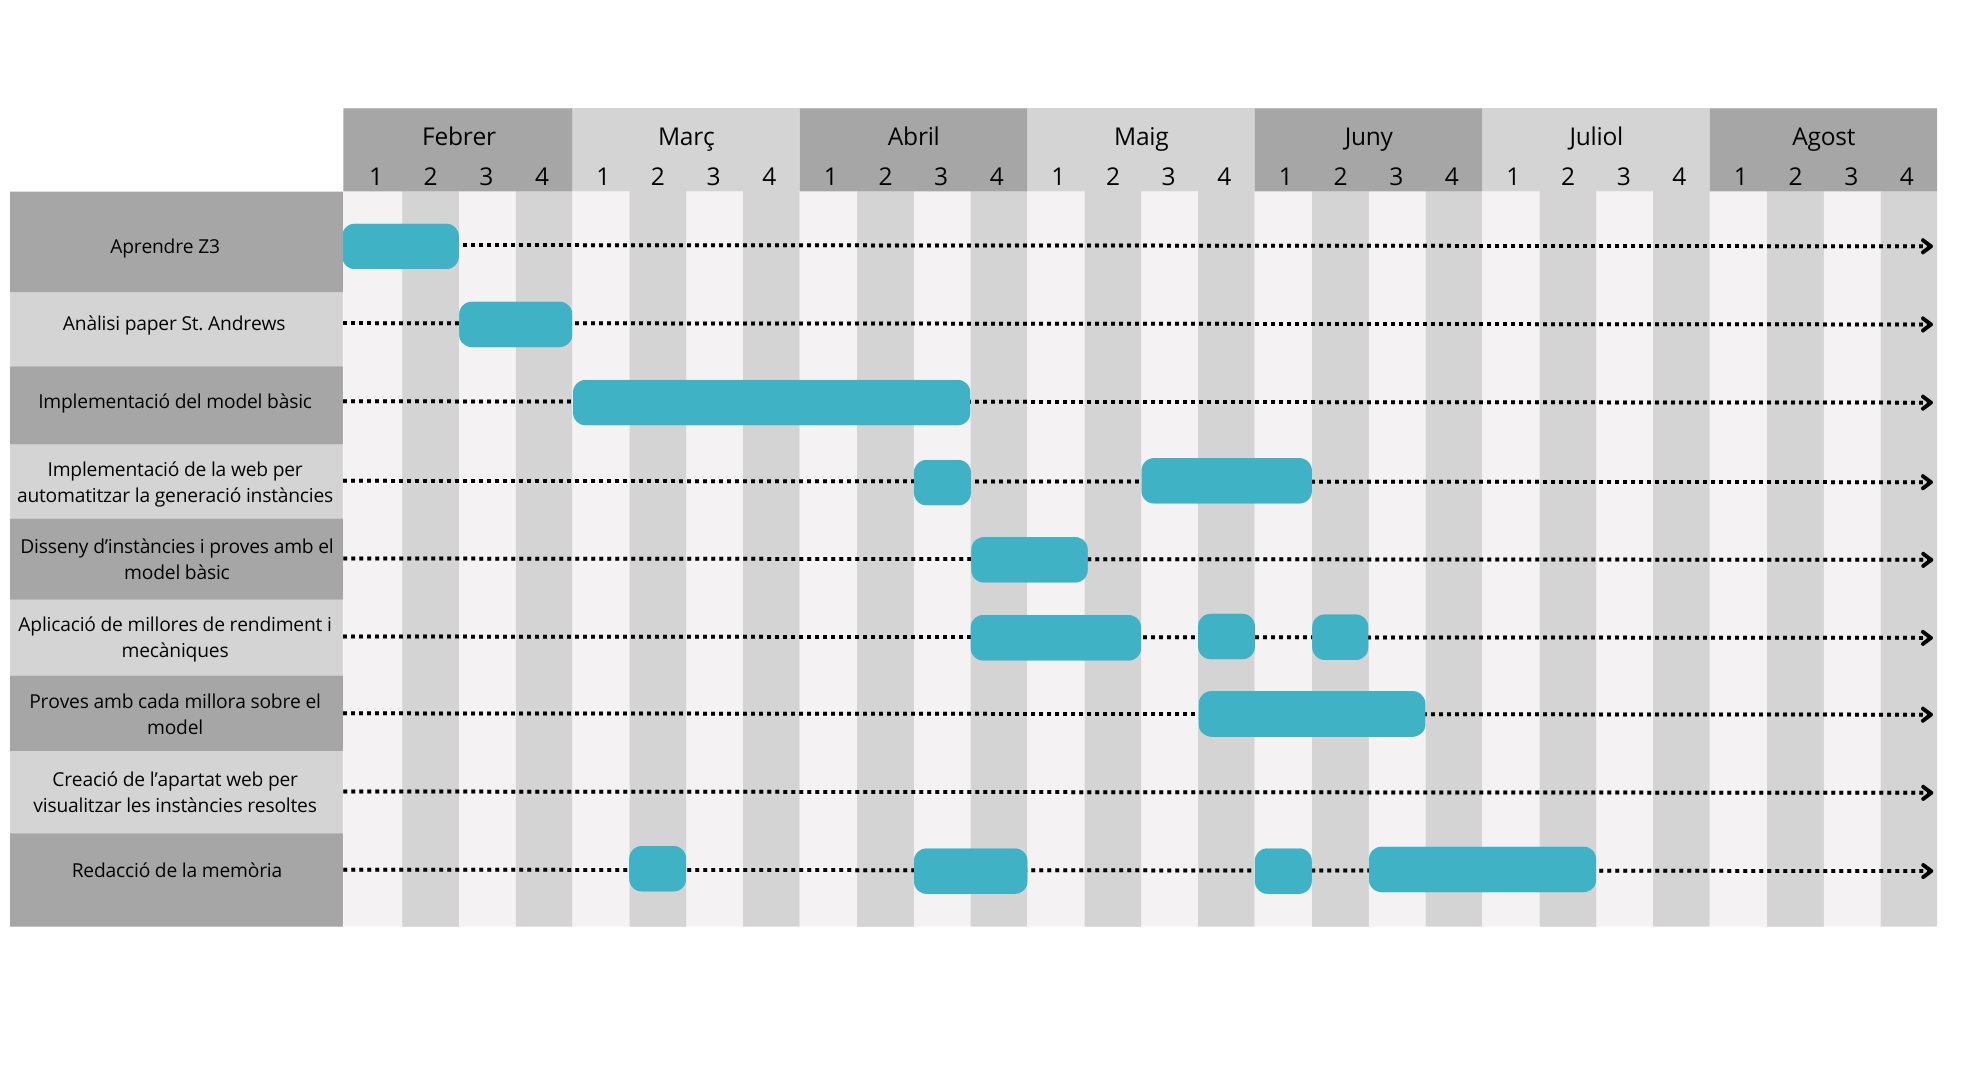
\includegraphics[width=1\linewidth]{Figures//miscelaneous/diagrama-grantt.png}
    \caption{Diagrama de Gantt del desenvolupament del projecte}
    \label{fig:diagrama-gantt}
\end{sidewaysfigure}

% Indicate the main file. Must go at the beginning of the file.
% !TEX root = ../main.tex

%----------------------------------------------------------------------------------------
% CHAPTER TEMPLATE
%----------------------------------------------------------------------------------------


\chapter{Marc de treball i conceptes previs} % Main chapter title

\label{Marc de treball i conceptes previs} % Change X to a consecutive number; for referencing this chapter elsewhere, use \ref{ChapterX}

%----------------------------------------------------------------------------------------
% SECCIÓ 1: Marc de treball i conceptes previs
%----------------------------------------------------------------------------------------
Aquí s'expliquen tots els conceptes que cal saber per poder entendre tot el que s'ha desenvolupat al projecte, des de la modelització fins al disseny web i la connexió client-servidor.
\section{Problemes de satisfacció de restriccions}
Els problemes de satisfacció de restriccions en anglès CSP, es defineixen com a un conjunt de n variables \( X = \{X_1, X_2, \ldots, X_n\} \), un conjunt \( D = \{D_1, D_2, \ldots, D_n\} \) de dominis per cada variable i un conjunt \( R = \{R_1, R_2, \ldots, R_n\} \) de restriccions aplicades sobre les variables del conjunt X, aquestes restriccions són relacions k àries entre les variables   on l'objectiu és trobar una assignació sobre el conjunt de variables X fent ús del domini D de cada variable que satisfaci totes les restriccions del conjunt R. Les assignacions de valors a les variables s'anomena interpretació, aquesta interpretació no té per què satisfer les restriccions imposades sobre les variables del conjunt X, però la interpretació que si satisfà totes les restriccions s'anomena model. Tot seguit un exemple del famós problema send more money:\\

Suposem que tenim les variables \( X = \{S, E, N, D, M, O, R, Y\} \) on el domini de cada variable és \( D = \{[0 .. 9], \ldots, [0 .. 9]\} \) i el que volem és satisfer la restricció \( R_1 = \{1000S + 100E + 10N + D + 1000M + 100O + 10R + E = 10000M + 1000O + 100N + 10E + Y\} \) a més també volem que tots els valors que prenguin les variables siguin diferents entre ells \( R_2 = \{alldiff(S, E, N, D, M, O, R, Y)\}\).\\
Una possible interpretació podria ser \(S=0, E=1, N=2, D=3, M=4, O=5, R=6, Y=7\) l'avaluació d'aquesta assignació sobre les restriccions seria:\\
$$ R_1 = \{4684 = 45217\} $$
$$ R_2 = \{alldiff(0, 1, 2, 3, 4, 5, 6, 7)\}$$\\
Aquesta interpretació no és model, ja que la restricció $R_1$ no se satisfà.\\
Una interpretació que sí que és model és la següent:
$$ S=9, E=5, N=6, D=7, M=1, O=0, R=8, Y=2 $$\\
Ja que satisfà les dues restriccions:\\
$$ R_1 = \{10652 = 10652\} $$
$$ R_2 = \{alldiff(9, 5, 6, 7, 1, 0, 8, 2)\}$$

Amb aquest exemple es pot veure com aquest tipus de problemes no tenen un ``mètode'' per ser resolts sinó que requereixen prova i error fins que no es topa amb la solució. La complexitat d'aquest tipus de problemes s'estudia a branca de la complexitat computacional, tot seguit s'expliquen les idees bàsiques sobre aquest camp de la computació.

\section{Complexitat computacional}
Per poder definir les diferents complexitats computacionals dels problemes de CSP, cal introduir el concepte de màquina de Turing la qual serveix de base per establir que és computable i que no.

\subsection{Màquina de Turing}
La màquina de Turing, inventada per Alan Turing el 1936, és un model de còmput que descriu la màquina més simple capaç de poder executar qualsevol algorisme informàtic. La màquina treballa amb un alfabet finit i consta d'una cinta de longitud infinita dividida en cel·les, cada cel·la pot contenir qualsevol símbol de l'alfabet. La màquina també compta amb un capçal el qual apunta a la cel·la actual i és capaç de fer operacions de lectura i escriptura sobre la cel·la que apunta. A més la màquina compta amb un conjunt finit d'estats i una taula finita d'instruccions, en funció del símbol llegit i l'estat actual, s'escull una de les instruccions de la taula que poden ser, moure el capçal a la dreta o esquerra, esborrar o escriure un símbol a la cel·la actual o bé canviar d'estat.

\subsection{Classes de complexitat}
A la teoria de la computació hi ha moltes classes de complexitat, referents a l'espai en memòria necessari per resoldre un problema i el cost en temps requerit. Per aquest treball només s'explicaran les classes que fan referència al temps de còmput, ja que és el factor principal que afecta el problema de CSP.

\subsubsection{Classe P}
El conjunt de complexitat P conté tots aquells problemes que tenen un algorisme específic per ser resolts, on el cost en temps d'aquest algorisme augmenta polinomialment en funció del nombre de variables implicades al problema. Per exemple trobar el valor mínim en una llista de nombres té un cost lineal $O(n)$ que augmenta en funció de la longitud de la llista, l'ordenació dels nombres d'una llista és un altre problema de la classe P que pot ser resolt amb cost $O(n\log{}n)$ . També es diu que un problema és de complexitat P si una màquina de Turing determinista els pot resoldre en temps polinòmic.

\subsubsection{Classe NP i NP-complet} \label{np and np-completeness}
Els problemes de la classe NP (Nondeterminitic Polinomial Time), són aquells que poden ser resolts en temps polinòmic per una màquina de Turing no determinista, és a dir una màquina de Turing la qual de manera no determinista sap a quins estats ha de canviar per trobar la solució en temps polinòmic. L'exemple més conegut d'aquest tipus de problema tracta del problema de satisfacció (SAT) on donat un conjunt de variables booleanes i una CNF és volt trobar quina assignació fa que la CNF avaluï cert. A més SAT forma part de la classe NP-complet que implica que qualsevol problema NP pot ser reduït en temps polinòmic a SAT. Finalment, els problemes NP tenen la particularitat que una solució trobada pot ser verificada en temps polinòmic, per exemple per al problema SAT seria tan senzill com assegurar que cada clàusula avalua cert el qual tindria un cost lineal $O(n)$.

\subsubsection{NP-hard}
La classe NP-hard és de les més curioses, ja que la seva intersecció amb el conjunt NP forma el conjunt de la classe NP-complet, es poden reduir en temps polinòmic a NP-hard, però no tots els problemes NP-hard es poden reduir en temps polinòmic a problemes NP, a més, i molt important, els problemes NP-hard que no formen part del conjunt NP no es poden verificar en temps polinòmic per una màquina de Turing determinista. Per exemple alguns problemes d'optimització són NP-hard, ja que donada una solució comprovar que sigui l'òptima requereix saber totes les solucions per determinar si la solució trobada efectivament és l'òptima.\\
Totes aquestes definicions són certes sota l'assumpció que \(P\neq NP\) i fins que es pugui demostrar el contrari les classes de complexitat continuaran sent així. En cas que es pogués demostrar \(P = NP\), qüestió que tracta d'un dels set problemes del mil·lenni la representació de les classes de complexitat tenint en compte els dos escenaris pot ser vista a la figura \ref{fig:time-complexity-sets}.

\begin{figure}
    \centering
    
\includegraphics[width=1\linewidth]{Figures//miscelaneous/time-complexity-classes.png}
    \caption{Comparació de classes de complexitat si \(P\neq NP\) i \(P = NP\)}
    \label{fig:time-complexity-sets}
\end{figure}

\section{SAT}
Com s'ha explicat a la secció \ref{np and np-completeness}, SAT es troba dins el conjunt NP-complet, aquesta característica sumada a la simplicitat del problema, ha causat que sigui usat com a base per solucionar problemes del conjunt NP a causa de la propietat que tot problema del conjunt NP pot ser reduït a NP-complet. La tecnologia usada tracta dels SAT solvers els quals usen tècniques molt avançades per reduir el màxim el cost de la cerca per força bruta implícita als problemes d'aquesta complexitat.\\
Exemple del problema SAT.
Suposem que tenim la següent forma normal conjuntiva (CNF):\\
$$(a \lor b \lor c) \land (\lnot c \lor \lnot b) \land (\lnot a \lor \lnot b) \land (\lnot a \lor \lnot c) $$\\
Una interpretació possible seria:\\
$$ [a = cert, b = false, c = false]$$
$$(cert \lor false \lor false) \land (\lnot false \lor \lnot false) \land (\lnot cert \lor \lnot false) \land (\lnot cert \lor \lnot false) $$
$$cert  \land (cert \lor cert) \land (fals \lor cert) \land (fals \lor cert) $$
$$cert \land cert  \land cert \land cert $$
$$\textbf{cert}$$\\
Aquesta satisfà la fórmula, és model. A més aquesta CNF té la propietat que les assignacions que satisfan la fórmula són aquelles on només un literal és cert.\\
\begin{table}
    \centering
    \begin{tabular}{ccc|c}
        $a$ & $b$ & $c$ & $(a \lor b \lor c) \land (\lnot a \lor \lnot b) \land (\lnot a \lor \lnot c) \land (\lnot b \lor \lnot c)$ \\
        \hline
        1 & 1 & 1 & 0 \\
        1 & 1 & 0 & 0 \\
        1 & 0 & 1 & 0 \\
        1 & 0 & 0 & 1 \\
        0 & 1 & 1 & 0 \\
        0 & 1 & 0 & 1 \\
        0 & 0 & 1 & 1 \\
        0 & 0 & 0 & 0 \\
    \end{tabular}
\end{table}


Un dels problemes de SAT és que com que tracta de la satisfacció de les clàusules d'una CNF les quals estan formades per literals que són variables booleanes, hi ha problemes sobretot si aquests tracten amb variables numèriques que són molt difícils de reduir a SAT i encara que siguin reduïbles en certs casos generen tantes clàusules que usar un SAT solver passa a ser una opció inviable. Hi ha diverses alternatives que permeten fer modelitzacions similars a les que es farien amb SAT, però amb l'opció de poder usar variables de diferents tipus, per aquest projecte s'ha usat SMT (SAT Modulo Theories).

\section{SMT}
SMT o SAT Modulo Theories, tracta del problema de determinar si una fórmula matemàtica és satisfacible. A diferència del problema SAT, SMT incorpora múltiples teories, des d'aritmètica lineal fins a comparacions lògiques entre funcions no interpretades. Aquestes teories permeten l'ús de diferents tipus de dades (enters, reals, strings, llistes, arrays de bits...). A més també permet crear fórmules lògiques igual que a SAT però amb l'ús de les teories.\\
\begin{figure}
    \centering
    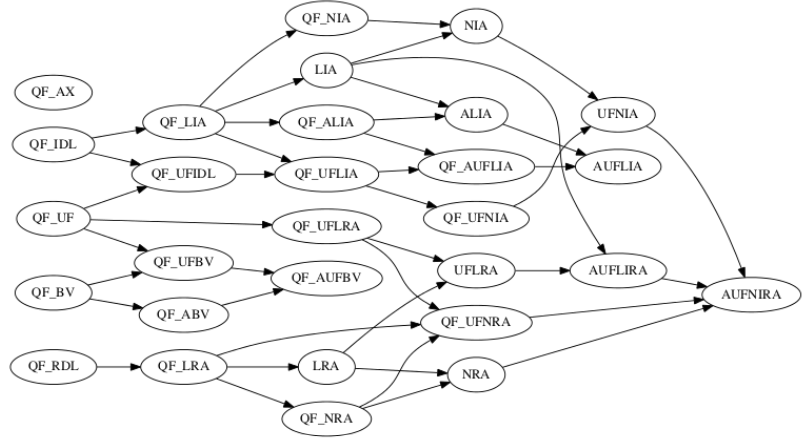
\includegraphics[width=0.5\linewidth]{Figures//miscelaneous/smt-lib-theories.png}
    \caption{Teories suportades per SMT-lib \cite{SMT-solving}}
    \label{fig:smt-theories}
\end{figure}

Els SAT solvers tenen un nucli que està especialitzat a trobar les assignacions satisfacibles de la fórmula fent ús de tècniques com CDCL. SMT aprofita aquest nucli i en fa una abstracció incorporant l'ús de les teories, tot seguit un exemple per entendre millor l'abstracció.
Suposem que tenim la següent fórmula:

$$ (c \le 5) \land (a \geq 3) \land (5a+b=c-3) $$
El primer pas és identificar cada teoria present a la fórmula i abstreure'n una variable booleana perquè el nucli SAT pugui resoldre.\\
$$ [A=(c \le 5), B=(a \geq 3), C=(5a+b=c-3)] $$
$$ A \land B \land C $$

Dins de les teories que la llibreria de SMT-lib suporta \ref{fig:smt-theories}, les variables A i B tracten de la teoria (integer rational difference logic o QF\_IDL) i la variable C la teoria (real/integer linear arithmetic). Amb l'abstracció feta i les teories identificades el solver primer resol la part SAT de la fórmula, si es troba una assignació vàlida es criden els nuclis que resolen les teories, en cas que hi hagi una assignació que satisfaci les variables abstretes la fórmula és satisfacible, en cas contrari, el nucli del SAT solver aprèn com a lema que la variable no pot ser assignada un valor positiu i continua fent solving fins que es demostra satisfacibilitat o no hi ha més assignacions disponibles.\\
En aquest exemple com la fórmula és molt simple el SAT solver demana als nuclis de les teories esmentades que avaluïn cert i aquestes per exemple podrien respondre el següent:
$$ A \Rightarrow c=4 \Rightarrow 4\le5 \Rightarrow cert $$
$$ B \Rightarrow a=3 \Rightarrow 3\geq5 \Rightarrow cert $$
$$ C \Rightarrow b=-14 \Rightarrow (15-14=4-3) \Rightarrow cert $$
L'esquema de la figura \ref{fig:smt-solver-lazy} representa el procés de solving d'un SMT solver usant lazy solving.
\begin{figure}[H]
    \centering
    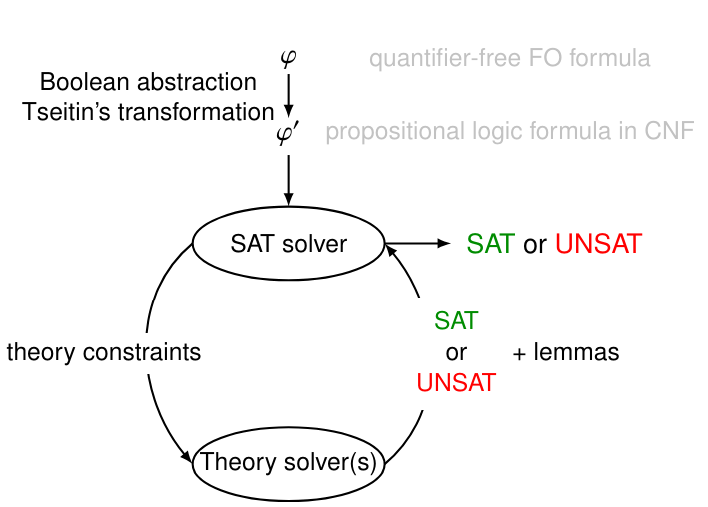
\includegraphics[width=0.5\linewidth]{Figures//miscelaneous/smt-lazy-zolver.png}
    \caption{Esquema d'un SMT solver lazy \cite{SMT-solving}}
    \label{fig:smt-solver-lazy}
\end{figure}

\section{Elements bàsics del joc Factorio}
Com s'ha explicat prèviament, Factorio és un joc d'automatització i ampliació de fàbriques en un món 2D basat en una graella. Els elements que el joc posa a disposició del jugador en són molts, així i tot, els bàsics per poder construir i automatitzar la producció d'objectes en són tres: inseridors, cintes transportadores i assembladors tot seguit una explicació en detall del comportament de cadascun.

\subsection{Cinta transportadora}
Les cintes transportadores o \textit{conveyor belts} serveixen per transportar elements d'un punt a un altre. Aquestes ocupen 1x1 caselles a la graella del món i poden prendre qualsevol de les 4 direccions cardinals. Transporten objectes de la casella actual a la següent casella apuntada per la cinta. Aquestes poden rebre objectes per qualsevol de les tres caselles adjacents diferents de la casella de sortida (la que apunta la cinta).
Al joc les cintes consten de dues pistes cadascuna amb la mateixa capacitat de transport d'objectes, però no s'ha tingut en compte aquesta mecànica, ja que de la manera que funciona afegeix molta complexitat.
La capacitat de transport d'una cinta, tenint només en compte una de les pistes, és de 450 objectes per minut.
\begin{figure}[ht]
    \centering
    \begin{subfigure}{0.45\textwidth}
        
\includegraphics[width=\textwidth]{Figures/captures_joc/conveyor.png}
        \caption{Cinta transportadora a la graella del joc}
    \end{subfigure}
    \hfill
    \begin{subfigure}{0.45\textwidth}
        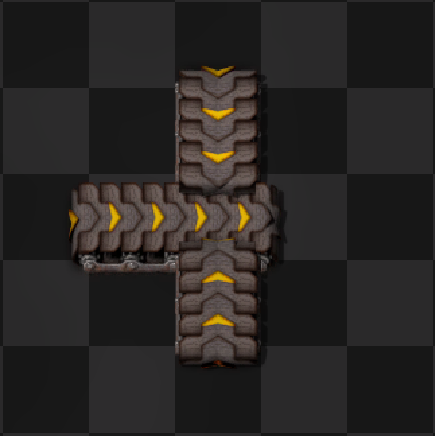
\includegraphics[width=\textwidth]{Figures/captures_joc/conveyor_inputs.png}
        \caption{Entrades permeses a una cinta transportadora}
    \end{subfigure}
    \caption{Cinta transportadora dins el joc i les seves possibles entrades}
    \label{fig:conveyor_in_out}
\end{figure}

\subsection{Inseridor}
Els inseridors o \textit{inserters} són braços robòtics que ocupen 1x1 caselles a la graella del món, permeten inserir i treure elements de cintes i assembladors.\\
Aquests poden treure elements de cintes que apuntin en qualsevol direcció i inserir objectes a cintes que no apuntin cap a ell. L'inseridor és l'únic element que pot suplir d'objectes a un assemblador i té el hàndicap que la seva capacitat de transport és de 50 objectes per minut.

\begin{figure}[H]
    \centering
    
\includegraphics[width=0.33\linewidth]{Figures/captures_joc/inserter.png}
    \caption{Inseridor a la graella del joc}
    \label{fig:in_game_inserter}
\end{figure}


\begin{figure}[h]
    \centering
    \begin{subfigure}{0.45\textwidth}
        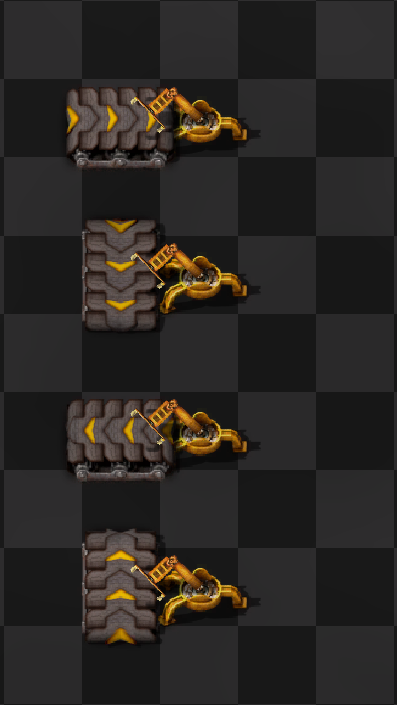
\includegraphics[width=\textwidth]{Figures/captures_joc/inserter_allowed_inputs.png}
        \caption{Entrades permeses}
    \end{subfigure}
    \hfill
    \begin{subfigure}{0.45\textwidth}
        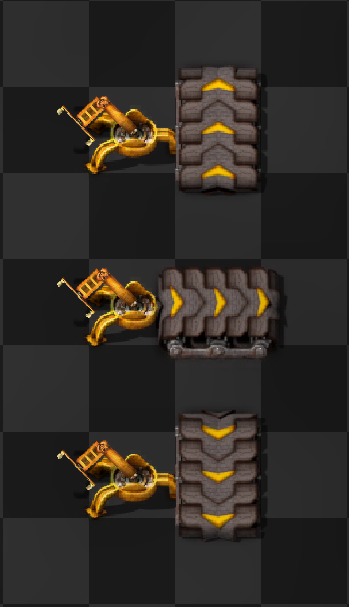
\includegraphics[width=\textwidth]{Figures/captures_joc/inserter_allowed_outputs.png}
        \caption{Sortides permeses}
    \end{subfigure}
    \caption{Orientacions de les cintes d'on un inseridor pot treure i agafar objectes}
    \label{fig:inserter_in_out}
\end{figure}

\subsection{Assemblador}
Els assembladors o \textit{assemblers} ocupen un espai de 3x3 caselles a la graella del món, aquests només poden rebre i treure objectes a través d'inseridors que estiguin en el mateix eix que qualsevol de les 12 caselles adjacents a l'assemblador.\\
La funcionalitat dels assembladors és convertir els materials d'entrada en objectes refinats, això es fa mitjançant receptes.

\begin{figure}[h]
    \centering
    \begin{subfigure}{0.45\textwidth}
        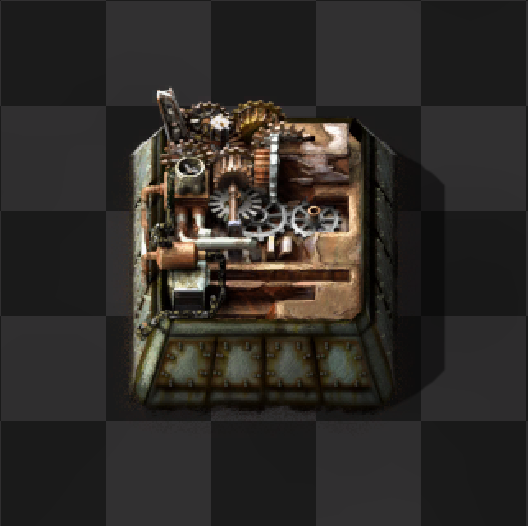
\includegraphics[width=\textwidth]{Figures/captures_joc/assembler.png}
        \caption{Assemblador a la graella del joc}
    \end{subfigure}
    \hfill
    \begin{subfigure}{0.45\textwidth}
        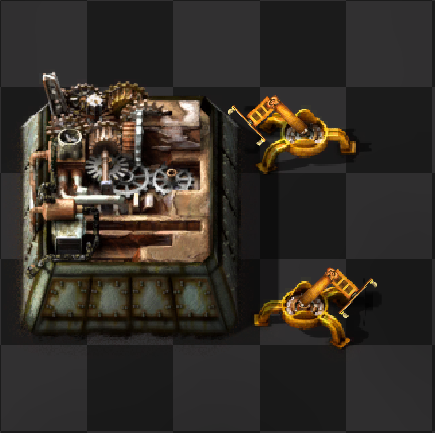
\includegraphics[width=\textwidth]{Figures/captures_joc/inserters_assembler.png}
        \caption{Inseridors interactuant amb l'assemblador}
    \end{subfigure}
    \caption{Representació de l'assemblador dins el joc}
\end{figure}

\subsubsection{Receptes} \label{subsec:recipes}
Les receptes només poden estar associades als assembladors, aquestes indiquen quins i quants objectes són necessaris per a la fabricació d'un altre objecte en un temps determinat.\\
Amb el temps que tarda un assemblador a produir els objectes d'una recepta i la quantitat d'objectes que requereix, podem calcular el nombre d'objectes per minut d'entrada i sortida màximes d'una recepta. Això ens serà molt útil més endavant per modelar receptes i el flux d'objectes.\\
En cas que un assemblador rebi més objectes per minut dels requerits per la recepta, aquests s'acumularan als inseridors i cintes que transporten l'objecte a l'assemblador, d'altra banda, si l'assemblador rep menys objectes per minut del que la recepta requereix, l'assemblador haurà d'esperar a tenir els objectes per iniciar la recepta fent que velocitat dels objectes fabricats es redueixi.\\
Totes les receptes que es produeixen a l'assemblador sempre generen un sol tipus d'objecte de sortida.

\begin{figure}[H]
    \centering
    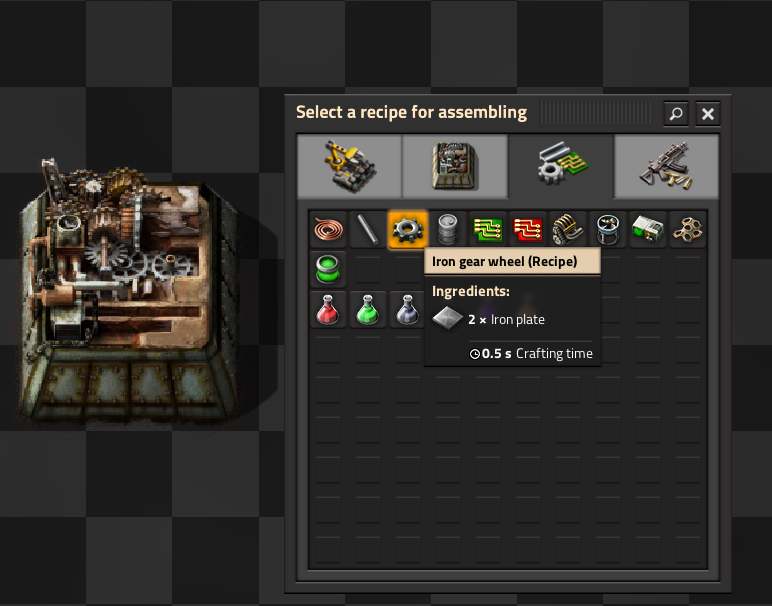
\includegraphics[width=0.5\linewidth]{Figures/captures_joc/assembler_recipe.png}
    \caption{Informació de la recepta d'un assemblador}
    \label{fig:assembler_recipe}
\end{figure}

\section{Conceptes relacionats amb els elements bàsics del joc}
Amb elements bàsics que poden constituir un \textit{blueprint} ja explicats, queda definir com aquests elements han d'interactuar entre ells per formar una fàbrica que respecti les mecàniques del joc, així doncs tot seguit s'explica com s'han dividit les interaccions entre elements, objectes que és es produeixen a la fàbrica...

\subsection{Ruta}
Una de les parts més importants del model és definir com la concatenació d'inseridors i cintes transportadores conformen una ruta. Perquè una ruta sigui vàlida no pot crear cicles, és a dir que una cinta o inseridor no pot entrar objectes a una cinta la qual era anterior a ella mateixa. També s'ha de tenir en compte l'orientació dels inseridors i cintes per complir amb les entrades i sortides vàlides anteriorment descrites. Una ruta també es pot bifurcar i unir.\\
Els inicis de ruta poden ser les caselles marcades com a entrada o bé la sortida d'un objecte d'un assemblador. D'altra banda, els finals de ruta poden ser les caselles marcades com a sortida o bé l'inseridor que afegeix elements a un assemblador.

\subsection{Tipus d'objectes}
Les cintes i inseridors han de poder dur objectes per les rutes que conformen, aquí entra la noció del tipus d'objectes, que depenen dels d'objectes especificats a les caselles d'entrada i sortida del \textit{blueprint}, juntament amb els objectes que un assemblador genera en funció de la recepta que tingui associada. Cal assegurar que a les 12 caselles adjacents a un assemblador les quals tenen inseridors entrant o sortint, no duguin o treguin objectes que la recepta associada a l'assemblador demana, també cal assegurar que una casella que forma part d'una ruta només pot dur un tipus d'objecte i finalment cal assegurar la correcta propagació dels objectes per les rutes.

\subsection{Quantitat d'objectes}
A banda de portar objectes, les rutes poden estar més o menys carregades, és a dir que cal alguna manera de saber quants objectes per minut porta una cinta o inseridor per poder saber quants objectes per minut ha de produir la recepta associada a un assemblador.\\
La recepta associada a un assemblador, com bé ha quedat explicat anteriorment, requereix un cert nombre d'objectes per minut per produir-ne uns altres a una densitat específica. Un dels problemes principals és que un assemblador pot rebre objectes requerits per la recepta en diferents quantitats que poden ser superiors o inferiors a la ràtio que marca la recepta, però els objectes que entrin en major quantitat no ho podran fer durant gaire temps, ja que ràpidament l'assemblador se saturarà d'objectes fent que la quantitat d'entrada s'anivelli a la quantitat respectiva de l'objecte que crea el coll d'ampolla.\\
Determinar correctament la quantitat d'objectes que hi ha a cada casella del \textit{blueprint} és una de les parts més crucials del problema, ja que és la que ens permetrà saber quants elements s'estan produint, cosa que volem maximitzar.

\section{El problema del blueprint} \label{sec:blueprint_problem}
El problema que es vol resoldre s'anomena el problema del \textit{blueprint}, el qual donades les entrades i sortides dels objectes, l'objecte que es vol produir i l'espai del qual es disposa, s'ha de maximitzar la quantitat produïda de l'objecte de sortida.\\
Per entendre millor apartats futurs on es parla d'implementacions concretes, es presenta un exemple, el qual tracta d'una instància resolta pel model. Amb aquest exemple es posa en context el problema i s'explica perquè aquest no és gens senzill.

\subsection{Exemple del problema}
Els inputs d'aquesta instància són les següents:\\
\begin{itemize}
    \item Mida: 8x8
    \item Entrades: (0,0) ``quadrat gris'' Xapes de ferro, (0,7) ``quadrat vermell'' Xapes de coure, (7,0) ``quadrat blanc'' Barres de plàstic
    \item Sortides: (7,7) ``cercle taronja'' Circuits avançats
    \item Objecte a produir: Circuits avançats
\end{itemize}

\begin{figure}
    \centering
    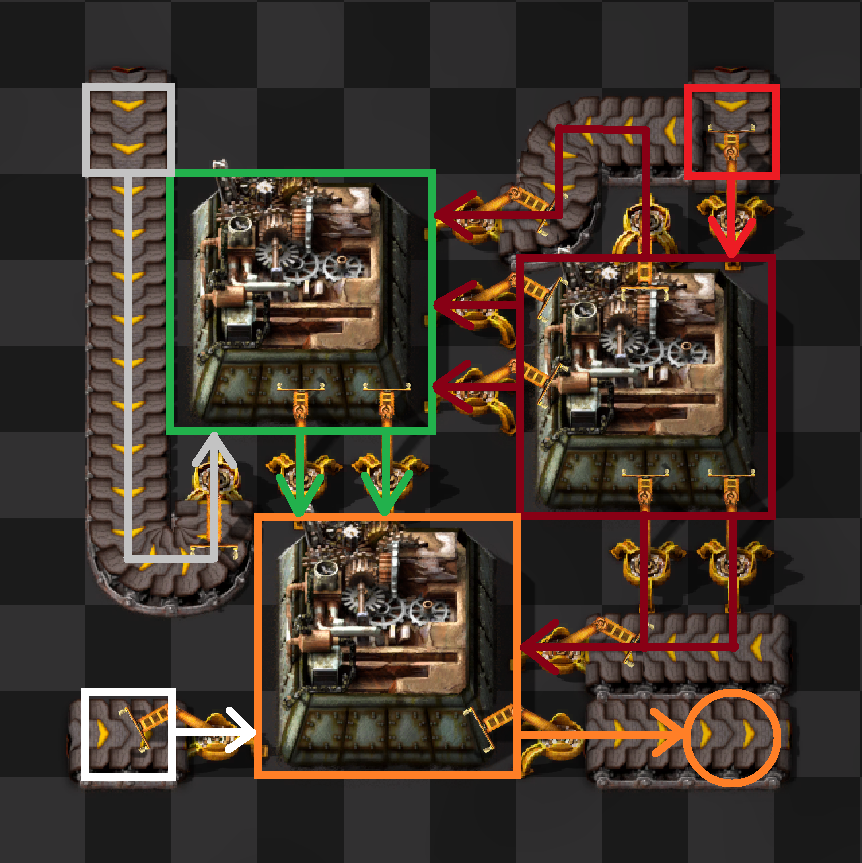
\includegraphics[width=0.75\linewidth]{Figures//captures_joc//exemples_model/exemple_base.png}
    \caption{Exemple base}
    \label{fig:solucio_exemple}
\end{figure}

Com es pot veure a l'exemple resolt \ref{fig:solucio_exemple}, per produït Circuits avançats s'han necessitat tres assembladors, un per cada recepta implicada en la producció de Circuits avançats, concretament es requereixen les receptes:
\begin{itemize}
    \item Cable de coure "assemblador emmarcat en carmí"
    \item Circuits electrònics "assemblador emmarcat en verd"
    \item Circuits avançats "assemblador emmarcat en taronja"
\end{itemize}


Com l'espai del \textit{blueprint} és molt ajustat hi ha rutes que només tracten d'un inseridor que agafa els objectes produïts d'un assemblador i els insereix directament al assemblador adjacent.\\

Pel que fa a la distribució dels objectes primer cal saber la quantitat d'objectes per minut que requereix i produeix cada recepta.\\
\begin{table}
\centering  
\begin{tabular}{|c|c|c|}
\hline
\textbf{Recepta} & \textbf{Requereix} & \textbf{Produeix} \\ \hline

Circuit avançat & 
\begin{tabular}{@{}c@{}}
40 Cable de coure \\ \hline
20 Circuits electrònics \\ \hline
20 Barres de plàstic
\end{tabular} &  
10 Circuits avançats
\\ \hline

Circuit electrònic &
\begin{tabular}{@{}c@{}}
360 Cable de coure \\ \hline
120 Plaques de ferro \\ \hline
20 Barres de plàstic
\end{tabular} &
120 Circuits electrònics \\ \hline

Cable de coure & 120 Plaques de coure & 240 Cables de coure \\ \hline
\end{tabular}\\
\caption{Materials requerits i produïts per cada recepta}
\label{table:objectes_requerits}
\end{table}
Pel que fa als materials en cru que entren per les caselles emmarcades a la imatge, estan entrant les següents quantitats:

\begin{table}
    \centering
    \begin{tabular}{|c|c|}
        \hline
        \textbf{Material} & \textbf{Quantitat d'entrada} \\ \hline
        Placa de coure & 50\\ \hline
        Placa de ferro & 98.06\\ \hline
        Barra de plàstic & 20.0138\\ \hline
    \end{tabular}
\end{table}

D'aquestes quantitats d'entrada no s'aprofiten tots els objectes pel fet que alguns assembladors no tenen prou inseridors de sortida per poder aprofitar tot el material. Aquesta ``pèrdua'' es tradueix en material que s'acumula a les cintes d'on els inseridors agafen els materials d'entrada pel assembladors, concretament la cinta a la posició (7,0) acumula 0.138 barres de plàstic, fent que la quantitat d'entrada de l'assemblador de circuits avançats sigui de 20 barres de plàstic per minut. D'altra banda, la cinta a la posició (5,1) acumula 78.06 plaques de ferro, fent que l'entrada a l'assemblador sigui de 20 plaques de ferro per minut. Finalment, les plaques de coure que entren per la casella (0,7) s'aprofiten totes.\\

Ara que ja s'han explicat les quantitats d'entrada i els materials que cada recepta requereix, es pot veure com l'assemblador carmí per poder processar les 50 plaques de coure per minut ha de poder extreure 100 cables de coure això ho fa mitjançant 5 inseridors, els quals es divideixen la quantitat de sortida en parts proporcionals fent que $3/5$ parts, és a dir 60 cables, es destinin a la producció de circuits electrònics i $2/5$ parts, és a dir 40 cables, es destinin a la producció de circuits avançats.\\
Els cables destinats a la producció de circuits electrònics s'aprofiten tots, ja que l'entrada de plaques de ferro és de 20/min i com s'ha vist a la taula \ref{table:objectes_requerits} per cada placa de ferro es necessiten tres cables de coure, així que per 20 plaques de ferro s'entren 60 cables de coure, produint 20 circuits electrònics per minut. Aquests 20 circuits electrònics s'aprofiten tots per la recepta de circuits avançats juntament amb les 20 barres de plàstic d'entrada i la resta de cables de coure, fent que l'assemblador que produeix circuits electrònics funcioni al 100\% de rendiment, fent que si es volguessin produir més circuits avançats es requerís un segon assemblador el qual per les dimensions del \textit{blueprint} no sigui viable.\\

Amb aquest exemple es pot entendre més la complexitat del problema i la quantitat de factors que hi juguen. A més també serveix per ser usat com a ajuda visual per entendre implementacions específiques en apartats posteriors.



% Indicate the main file. Must go at the beginning of the file.
% !TEX root = ../main.tex

%----------------------------------------------------------------------------------------
% CHAPTER TEMPLATE
%----------------------------------------------------------------------------------------


\chapter{Requisits del sistema} % Main chapter title

\label{Requisits del sistema} % Change X to a consecutive number; for referencing this chapter elsewhere, use \ref{ChapterX}

%----------------------------------------------------------------------------------------
% SECCIÓ 1: Requisits del sistema
%----------------------------------------------------------------------------------------
Per aquest projecte s'han usat dues llibreries principals que separen el treball en dues parts. Front end, es tracta de la web on es poden generar i visualitzar instàncies, back end fet en Python que conté tota la lògica i les modelitzacions.\\
Com és un projecte fet en Python els requisits són molt fàcils d'instal·lar en un ordinador sense importar si el sistema operatiu és Windows o Linux. Els passos a seguir són:
\begin{enumerate}[label=Pas \arabic*:]
\item Tenir una màquina amb un intèrpret de Python amb la versió 3.9
\item Crear un entorn virtual amb la comanda \lstinline{python -m venv <directory>}
\item Activar l'entorn virtual mitjançant la comanda \lstinline{venv\\Scripts\\activate.bat} des d'un terminal cmd o \lstinline{source myvenv/bin/activate} des d'un sistema Linux o MacOS.
\item Clonar el repositori en un directori nou dins el directori on s'ha creat l'entorn virtual, l'estructura de fitxers hauria de ser la següent: 
    \begin{verbatim}
    projecte/
        venv/                     # entorn virtual
        FactorioPlanner/          # repositori clonat
            script.py
            requirements.txt
            ...
    \end{verbatim}
\item Situar-se al directori principal del projecte i executar la comanda \lstinline{pip install -r requisits.txt}, aquesta comanda instal·larà totes les dependències del projecte a l'entorn virtual.
\item Executar la comanda \lstinline{python mainWeb.py} per iniciar el servidor.
\item Connectar-se al servidor localment des de qualsevol navegador usant l'URL \lstinline{http://127.0.0.1:5000/}.
\end{enumerate}

A continuació es fa una explicació més en detall de les llibreries principals que formen part dels requisits:

\section{Z3}
Z3 com s'ha explicat per sobre a l'anterior apartat tracta d'un llenguatge de modelització de constraints. La peculiaritat del Z3 és que tracta d'un SMT (Satisfiability Modulo Theories) és a dir generalitza el problema SAT, afegint diferents teories (funcions no interpretades, àlgebra lineal, arrays...) al problema de satisfacció booleana.\\

Per aquest treball s'ha usat l'API de Z3 des de Python, a causa que al llarg de l'informe s'exposaran múltiples talls de codi, tot seguit es fa una explicació de com s'usen els operadors lògics i defineixen variables Z3 des de Python.

\subsection{Tipus i declaració de variables}
Z3 té molts tipus de variables (reals, enters, arrays, bit vectors, booleanes, uninterpreted functions i tipus finits customizables), per declarar aquestes variables és molt senzill, simplement cal usar el constructor donat pel Z3. Una funció molt interessant és que en usar Python com a llenguatge podem guardar les nostres variables en qualsevol mena d'estructura de dades, cal tenir en compte, que l'accés a aquestes estructures només es pot fer mitjançant variables Python així que si cal accedir a una posició d'una matriu en funció del valor pres per una variable Z3, haurem d'usar la teoria dels Arrays.\\
Per últim i molt important, el domini de les variables no es defineix a l'hora de declarar-les, sinó que cal definir restriccions que acotin el domini de la variable, crear un tipus enumerat amb el domini preestablert o usar bit vector amb un nombre determinat de bits.
Tot seguit exemples de declaració de diferents tipus de variables.

\begin{lstlisting}[language=Python, caption=Declaració de variables]
real = Real("real_variable")
enter = Int("integer_variable")
bit_vector = BitVec("bit_vector_variable", n_bits)
array = Array("array_variable", IntSort(), IntSort())
function = Function("function_variable", IntSort(), BoolSort())
bool = Bool("boolean_variable")
color_type, colors = EnumSort("color", ["blue", "orange", "green", "yellow", "red"])
\end{lstlisting}

Alguns detalls importants són que els BitVectors necessiten el nombre de bits com a paràmetre, també que aquests es poden interpretar com a nombres amb signe o sense, per diferenciar-ne el tipus és important usar l'operador correcte a l'hora de definir les restriccions sobre variables del seu tipus, més endavant s'ensenyen les diferències.\\
Les funcions i els Arrays requereixen el tipus de variable amb el qual indexen o prenen com a paràmetre i també el tipus que han de retornar, això s'indica posant ``Sort'' després del tipus que es vol que prenguin o retornin.\\

Com s'ha explicat les variables Z3 es poden guardar en estructures Python, aquí un exemple de com es guardarien les files del problema de les n-reines.
\begin{lstlisting}[language=Python, caption=Variables Z3 en arrays de Python]
queens = [Int(f"Q_{row + 1}") for row in range(n_queens)]
\end{lstlisting}
En aquest cas s'usen les llistes per comprensió de Python per declarar un Array amb variables enteres Z3.

\subsection{Operadors lògics}
Per construir fórmules lògiques necessitem l'ús d'operadors lògics. Des de l'API de Python es proporcionen mètodes per cada operador, alguns d'aquests no són tan visualment entenedors com els d'altres llenguatges centrats en constraint programming com MiniZinc o EssencePrime, així i tot, a continuació es fa una comparació entre els operadors lògics i els de l'API de Z3.

\begin{table}[h]
\centering
\begin{tabular}{|c|c|c|}
\hline
\textbf{Operador} & \textbf{Z3} \\
\hline
$a \land b$ & \verb|And(a, b)|  \\
\hline
$a \lor b$ & \verb|Or(a, b)|  \\
\hline
$\lnot a$ & \verb|Not(a)|  \\
\hline
$a \oplus b$ & \verb|Xor(a, b)|  \\
\hline
$a \Rightarrow b$ & \verb|Implies(a, b)|  \\
\hline
$a \Leftrightarrow b$ & \verb|a == b|  \\
\hline
$a > b$ & \verb|a > b, UGT(a, b)|  \\
\hline
$a < b$ & \verb|a < b, ULT(a, b)|  \\
\hline
$a \geq b$ & \verb|a >= b, UGE(a, b)|  \\
\hline
$a \leq b$ & \verb|a <= b, ULE(a, b)|  \\
\hline
$a \neq b$ & \verb|a != b|  \\
\hline
\end{tabular}
\caption{Comparació d'operadors lògics}
\label{tab:logic_oprator_comparison}
\end{table}

Com s'ha comentat anteriorment les variables de tipus BitVector requereixen operadors específics si es volen interpretar de manera ``unsigned'' per això els operadors ($>$, $<$, $\geq$, $\leq$) tenen les funcions (UGT, ULT, UGE i ULE), per les interpretacions unsigned dels BitVectors.\\

Finalment, una funcionalitat molt interessant de Z3 és que permet entrar llistes de variables als operadors lògics i aquests l'apliquen per totes les variables de la llista.\\
Per exemple:

\begin{lstlisting}[language=Python, caption=Variable Declaration]
int_variable = [Int(f"int_var_{i}") for i in range(10)]
less_than_ten = [int_variable[i] < 10 for i in range(10)]

all_and = And(less_than_ten)
all_or = Or(less_than_ten)
\end{lstlisting}

\section{Flask}
Flask és un framework desenvolupat en Python fàcil d'accedir des de la seva llibreria. El seu objectiu és proporcionar una interfície de servidor, facilitant mètodes simples per crear endpoints i comunicar de manera senzilla un client, amb el servidor.\\
En aquest projecte s'ha usat la llibreria per carregar tota la informació necessària de la pàgina web (html, css i fitxers Javascript), accedir a una col·lecció d'imatges per representar visualment les instàncies i per poder fer peticions al model desenvolupat i rebre els resultats.\\
Crear endpoints amb Flask és molt senzill tot seguit s'ensenya com.

\subsection{Crear Endpoints usant Flask}
Per crear un endpoint al nostre servidor és tan senzill com definir una funció estàndard de Python i usar un decorador específic per assignar la ruta.
\begin{lstlisting}[language=Python, caption=Declaració d'un endpoint]
from flask import Flask
app = Flask(__name__)
@app.route("/exemple")
def endpoint():
    print("endpoint d'exemple")
\end{lstlisting}

Amb aquesta funció creada i el servidor en marxa ja podem fer una petició al servidor usant l'adreça corresponent, si volem que el servidor ens torni informació podem ampliar la informació que afegim al decorador i especificar si es tracta d'un GET o un POST. Per exemple:\\

\begin{lstlisting}[language=Python, caption=Declaració d'un endpoint]
@_app.route('/processar', methods=['POST'])
def processar():
    data = request.get_json()
    resultat = processar_informacio(data)
    return jsonify(resultat)
\end{lstlisting}

D'aquesta manera es rep la informació del client en format JSON, s'extrau i se li aplica el procés que sigui necessari, finalment es passa en format JSON i es retorna al client.\\
El client pot estar implementat de moltes maneres, per aquest projecte s'ha optat per fer una pàgina web usant JavaScript. L'estructura de fitxers que ha de tenir el servidor ha de ser la següent.

\subsection{Estructura de fitxers}
Per poder guardar una pàgina web amb tots els elements que comporta (html, css i la lògica en JavaScript), es necessiten dos directoris. Un conté tots els htmls de les planes de la web i una altra contindrà la resta d'arxius que es vulguin guardar al servidor, imatges, fitxers d'estil html, dades en format JSON, scripts per la pàgina web...\\
A més el codi que llença el servidor s'ha de trobar al directori arrel i la resta de fitxers Python amb la lògica de l'aplicació es poden organitzar com es vulgui.
\begin{verbatim}
servidor/
    main.py               # llençador del servidor, endpoints...
    static/               # arxius, imatges, css, javascript...
        style.css
        weblogic.js
        images/
    templates/            # arxius html per la web
        index.html
    application/          # lògica, classes...
        app.py
        logic.py
\end{verbatim}

\subsection{Peticions des del client web}
Una de les maneres més estàndard de fer pàgines web és usant JavaScript. Per poder fer peticions des del client al servidor és necessari que es faci de manera asíncrona per no bloquejar la funcionalitat de la pàgina web mentre el servidor rep i processa la petició. Des de JavaScript enviar una petició es fa de la següent manera:

\begin{lstlisting}[language=Python, caption=Enviar petició]
function enviarPeticio() {
    let data = "informacio"

    fetch('/processar', {
        method: 'POST',
        headers: {
            'Content-Type': 'application/json',
        },
        body: JSON.stringify(data),
    })
    .then(response => response.json())
    .then(data => {
        console.log("El servidor ha respost correctament", data)
    })
    .catch((error) => {
        console.error('Error:', error);
    });
}
\end{lstlisting}

En aquesta funció s'està enviant una petició de tipus POST a l'endpoint \lstinline{/processar}, \lstinline{fetch()} és una funció asíncrona que rep com a paràmetres l'URL corresponent a l'endpoint del servidor i el contingut que contindrà el paquet enviat.\\
Un cop enviat el paquet, la resta del codi pot continuar i la funció \lstinline{then()} es queda a l'espera que \lstinline{fetch()} retorni la resposta del servidor. Si \lstinline{fetch()} respon, la primera funció \lstinline{then()} captura la informació enviada pel servidor, en cas que hi hagi un problema i el servidor no respongui o no es pugui llegir la informació enviada, \lstinline{catch()} llençarà un error informant que la petició ha fallat.



% Indicate the main file. Must go at the beginning of the file.
% !TEX root = ../main.tex

%----------------------------------------------------------------------------------------
% CHAPTER TEMPLATE
%----------------------------------------------------------------------------------------


\chapter{Estudis i decisions} % Main chapter title

\label{Estudis i decisions} % Change X to a consecutive number; for referencing this chapter elsewhere, use \ref{ChapterX}

%----------------------------------------------------------------------------------------
% SECCIÓ 1: Estudis i decisions
%----------------------------------------------------------------------------------------
Fins ara s'han explicat totes les tecnologies usades i les tasques que s'han desenvolupat al projecte, però no s'ha aprofundit en el perquè. En aquest apartat es dona una explicació del perquè de les decisions més importants, des de la selecció de llibreries fins a les diferents modelitzacions que s'han usat al model.

\section{Llibreria de solving}
Com ja s'ha explicat, al projecte s'han usat principalment dues llibreries, la més important tracta de Z3. El motiu principal pel qual s'ha escollit és perquè a l'article \cite{arxivpaper} el menciona a les propostes de millora. D'aquí s'ha fet una mica de recerca per saber-ne més i s'ha vist que és dels SMT solvers més reconeguts, a més el fet que estigui disponible per quasi tots els llenguatges de programació l'ha fet un candidat perfecte per desenvolupar el projecte. Per acabar de decidir-la com a llibreria per al projecte s'ha comentat al tutor i en Joan Espasa, membre del grup de recerca de la universitat de St. Andrews i col·laborador de l'article \cite{arxivpaper}, els quals han confirmat que es podia usar perfectament per desenvolupar el projecte.\\

\section{Llenguatge de programació}
La llibreria Z3 \cite{Z3Prover} està disponible per la majoria de llenguatges de programació. Entre ells s'hi troba Python que s'ha decidit usar per a aquest projecte, ja que és dels llenguatges on més ús es fa de la llibreria i on més recursos on-line es poden trobar. A banda el llenguatge en si és fàcil d'usar fent que a l'hora de modelitzar no sigui necessari preocupar-se de les particularitats del llenguatge.\\
A banda també s'ha escollit amb la idea en ment que en algun moment del projecte s'hauria d'implementar una interfície gràfica i Python té molts recursos per crear-les de manera fàcil.

\section{Interfície gràfica}
Des de l'inici es tenia clar que es volia fer alguna mena d'interfície gràfica per visualitzar les instàncies, ja que els models complexos que contenen moltes variables, interpretar els resultats sense cap mena d'eina que permeti visualitzar els valors presos de les variables es fa difícil.\\
En un bon principi es volia fer usant alguna llibreria gràfica de les que s'usen per crear videojocs com per exemple PyGame, però a mesura que el projecte ha evolucionat s'ha vist que a banda de crear una eina per poder visualitzar les instàncies resoltes també seria molt favorable crear-ne una altra per automatitzar-ne la generació. Això ha portat a la decisió que la millor opció era fer una web gràcies a la facilitat que té crear una interfície d'usuari amb botons, textos, entrada d'informació, descàrrega de fitxers, imatges, menús...\\
Arran d'aquesta decisió la creació de la visualització de les instàncies s'ha fet mitjançant l'element canvas que ofereix html, el qual és molt versàtil i fàcil de desenvolupar usant JavaScript.\\

\section{Connexió client servidor}
Aïllar la interfície gràfica del projecte, crea el problema que ja no es poden comunicar entre ells usant el mateix llenguatge. Per solucionar aquest problema s'ha decidit usar la llibreria Flask que permet connectar la web amb el model que resol les instàncies mitjançant la creació d'un servidor el qual pot rebre les peticions des de la interfície web. Aquesta clara separació de la part visual de la part lògica en un front end i un back end, ha fet que el projecte quedi més professional.\\
Aquí és on s'ha vist que la decisió d'escollir Python com a llenguatge de programació ha estat la correcta, ja que aquesta connexió client-servidor, s'ha pogut de manera molt simple i no ha causat els mals de cap que un altre llenguatge podria haver creat.

\section{Estructura del model}
Pel que fa al model, com s'ha comentat la idea bé de l'article \cite{arxivpaper} i la seva proposta a futur d'implementar-lo usant SMT. Tot i que hi ha conceptes que s'han usat al projecte que també es van usar a l'article \cite{arxivpaper}, aquest usava una estructura multinivell que causava la comprovació de solucions redundants, per això s'ha decidit unificar tots els nivells en un per ajudar al solver a propagar millor. Aquesta decisió ha comportat que bàsicament tot el model sigui completament diferent i a més degut a la incorporació de variables reals gràcies a la tecnologia SMT, hi ha mecàniques que no es van poder implementar a l'article \cite{arxivpaper}.\\

A banda l'objectiu d'optimització i les entrades del model respecte a l'article \cite{arxivpaper} també han canviat. S'ha decidit que la quantitat d'objectes que s'han d'entrar no sigui un input del model i que sigui el solver el que hagi de decidir, ja que en algunes instàncies és difícil determinar la quantitat que ha d'entrar de cada tipus així que s'ha decidit millor delegar la responsabilitat al solver.\\
A més com que s'ha pogut implementar de manera precisa la quantitat d'objectes a cada casella del \textit{blueprint}, s'ha decidit implementar una optimització addicional que redueix la pèrdua d'objectes al \textit{blueprint}, on pèrdua s'entén com la quantitat d'objectes que no s'estan aprofitant per produir altres objectes. Finalment, com a extra també s'ha afegit la possibilitat d'optimitzar la quantitat de cintes i inseridors que s'usen per transportar objectes.

\section{Instàncies}
Les entrades del model permeten crear moltíssimes instàncies, però per avaluar el rendiment s'ha decidit seguir un patró força estàndard, el que s'ha fet ha sigut separar les instàncies per mida de \textit{blueprint} des de 5x5 fins a 8x8. A més per cada mida s'han creat instàncies per diferents receptes les quals s'han ordenat de menys a més materials d'entrada requerits. Finalment, un cop feta la divisió entre mides i recepta, s'han creat múltiples instàncies variant les posicions per on entren els diferents materials i per on ha de sortir el material de la recepta objectiu.

% Indicate the main file. Must go at the beginning of the file.
% !TEX root = ../main.tex

%----------------------------------------------------------------------------------------
% CHAPTER TEMPLATE
%----------------------------------------------------------------------------------------


\chapter{Disseny del model} \label{disseny model} % Main chapter title

\label{Disseny del model} % Change X to a consecutive number; for referencing this chapter elsewhere, use \ref{ChapterX}
En aquest apartat s'expliquen totes les restriccions que conformen el model, des de la primera iteració del model, juntament amb les millores de comportament del model i les millores de rendiment aplicades. Per fer la lectura més còmoda els fragments de codi han estat alterats del llenguatge Python lleugerament en una mena de pseudocodi, a més també s'ha inclòs una versió simplificada de la formalització de cada restricció.

%----------------------------------------------------------------------------------------
% SECCIÓ 1: Implemenatció del model base
%----------------------------------------------------------------------------------------

\section{Implementació del model base}\label{model-base}

\subsection{Rutes}
Per implementar la noció de ruta s'ha usat la representació incremental on un element que forma part d'una ruta ha de precedir un element amb un valor de ruta inferior a ell i ser precedir per un element amb valor de ruta superior a ell. Per implementar aquesta representació s'ha creat una variable de tipus matriu \texttt{route} de mida $width \times height$, el seu domini també és $[0..width * height]$, ja que una ruta pot ocupar com a màxim tota l'àrea del \textit{blueprint}, a banda també cal saber l'orientació dels elements que formen part de la ruta (inseridors i cintes) les quals es guarden en dues variables una per cada element \texttt{conveyor} i \texttt{inserter} aquestes de la mateixa manera que la ruta són matrius de mida $width \times height$ i el seu domini $[empty, north, east, south, west]$ on \textit{empty} significa que no hi ha cap inseridor o cinta present. Amb aquestes variables ja es poden definir les restriccions que conformen una ruta, principalment en són dues:

\begin{table}[h]
    \centering
    \begin{tabular}{|c|c|c|}
    \hline
    \textbf{Variable} & \textbf{Mida} & \textbf{Domini} \\
    \hline
    route & $width \times height$ & $[0..width*height]$ \\
    \hline
    inserter & $width \times height$ & $[empty, north, south, east, west]$ \\
    \hline
    conveyor & $width \times height$ & $[empty, north, south, east, west]$ \\
    \hline
    \end{tabular}
    \caption{Variables implicades a les rutes}
    \label{route-variables}
\end{table}

\subsubsection{Augment de ruta}
Aquesta restricció ens codifica qualsevol element que formi part d'una ruta, ha de tenir una casella adjacent la qual el seu valor de la ruta sigui superior. En aquest cas les caselles adjacents vàlides només són les que estan en la mateixa direcció que la cinta o inseridor corresponent a la posició de la ruta. A banda també s'ha de tenir en compte que les rutes poden acabar si a la posició de la ruta hi ha un inseridor i en la direcció on aquest apunta hi ha un assemblador. A banda una ruta també pot acabar si la posició de la ruta es tracta d'una casella output donada com a entrada del model. En aquests dos casos no cal assegurar que la posició en la direcció de l'inseridor el valor de ruta sigui més gran. 

Finalment, la implementació de la restricció és la següent.
\begin{figure}
    \centering
    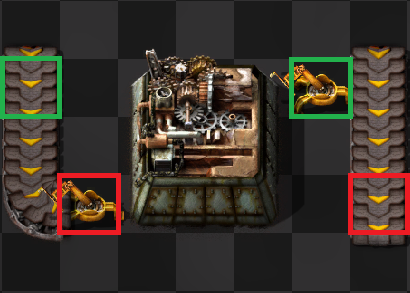
\includegraphics[width=0.5\linewidth]{Figures//captures_joc//exemples_model/start_end_pos.png}
    \caption{Possibles inicis ``verd'' i finals ``vermell" de rutes}
    \label{fig:start_end_route}
\end{figure}

\begin{lstlisting}[language=Python, caption=Forward Consistency]
for each cell (i, j) in the grid of size (height x width):
    if not is_output(i, j):
        inserter_output = []
        conveyor_output = []
        for each dir in [north, east, south, west]:
            x = i + displacement[dir][0]
            y = j + displacement[dir][1]
            if 0 <= x < height and 0 <= y < width:
                conveyor_output += If(conveyor[i][j] == dir,
                                      route[x][y] > route[i][j],
                                      False)
                                      
                inserter_output += If(And(inserter[i][j] == dir,
                                          assembler[x][y] == 0),
                                      route[x][y] > route[i][j],
                                      False)

                inserter_output += If(And(inserter[i][j] == dir,
                                          assembler[x][y] != 0),
                                      route[x][y] == 0,
                                      False)

            assert Implies(route[i][j] > 0, Or(conveyor_output + inserter_output))
\end{lstlisting}

La representació formal de la restricció seria la següent, per simplicitat només s'ha fet amb una direcció, però s'hauria de fer amb totes, a més s'ha simplificat l'if-then-else en una implicació lògica, però també caldria afegir la implicació amb la condició negada per representar l'else:
\begin{align*}
    &\forall i \in 0..width, \, \forall j \in 0..height, \\
    &((conveyor[i][j] == north) \rightarrow (route[i-1][j] > route[i][j])) \lor \\
    &((inserter[i][j] == north \land assembler[i-1][j] == 0) \rightarrow (route[i-1][j] > route[i][j])) \land \\
    &(inserter[i][j] == north \land assembler[i-1][j] !=0 ) \rightarrow (route[i-1][j] == 0)
\end{align*}

Cal mencionar que si les rutes només haguessin d'anar d'un punt A a un punt B amb aquesta restricció seria suficient per assegurar que no es creïn cicles i que realment s'està creant una ruta que va del punt A al B, però com que en el nostre cas les rutes s'han de poder bifurcar, unir i arribar des de múltiples punts a múltiples punts, cal la següent restricció.

\subsubsection{Decrement de ruta}
Per poder incloure bifurcacions i unions ens cal una restricció que de manera similar a l'anterior restricció ens asseguri que si una cinta o inseridor forma part d'una ruta i no es tracta d'un inici de ruta, llavors ha de tenir en una de les caselles veïnes, hi hagi un element de la ruta amb un valor inferior. Aquestes caselles veïnes seran diferents en funció de si l'element de la ruta tracta d'una cinta o un inseridor. Al cas de la cinta aquesta pot rebre input de qualsevol direcció que no sigui la mateixa que ella (Figura: \ref{fig:conveyor_in_out}) i en cas de l'inseridor aquest només pot rebre input de la casella en la direcció contrària a l'inseridor (Figura: \ref{fig:inserter_in_out}), a banda els inseridors també poder agafar objectes a un assemblador, així que en aquest cas forçarem que el valor de ruta a la posició de l'inseridor sigui 1 (inici de ruta).
Així doncs, la restricció queda de la següent manera:

\begin{lstlisting}[language=Python, caption=Backwards Consistency]
for each cell (i, j) in the grid of size (height x width):
    if not is_input(i, j):
        inserter_input = []
        conveyor_input = []
        for each dir in [north, east, south, west]:
            x = i + displacement[dir][0]
            y = j + displacement[dir][1]
            if 0 <= x < height and 0 <= y < width:
                conveyor_input += If(And(conveyor[i][j] != dir,
                                         conveyor[i][j] != empty),
                                     And(route[x][y] < route[i][j],
                                         route[x][y] > 0),
                                     False)
        
                inserter_input += If(And(inserter[i][j] == opposite(dir),
                                         assembler[x][y] == 0),
                                     And(route[x][y] < route[i][j],
                                         route[x][y] > 0),
                                     False)
        
               inserter_input += If(And(inserter[i][j] == opposite(dir),
                                        assembler[x][y] != 0),
                                    route[i][j] == 1,
                                    False)

    assert Implies(route[i][j] > 0, Or(conveyor_input + inserter_input))
\end{lstlisting}

\begin{align*}
    &\forall i \in 0..width, \, \forall j \in 0..height, \\
    &((conveyor[i][j] != north \land conveyor[i][j] != empty) \rightarrow \\
    &(route[i-1][j] < route[i][j] \land route[i-1][j]>0)) \lor \\
    &((inserter[i][j] == south \land assembler[i-1][j]==0) \rightarrow \\
    &(route[i-1][j] > route[i][j] \land route[i-1][j]>0)) \land \\
    &(inserter[i][j] == south \land assembler[i-1][j]!=0) \rightarrow \\
    &(route[i-1][j] == 1)
\end{align*}

Amb aquestes dues restriccions assegurem que la ruta no generi bucles i arribi als punts corresponents, però no ens assegura que l'orientació dels elements ni quins elements poden estar interconnectats entre si, així doncs per acabar de definit una ruta cal afegir quines entrades i sortides són vàlides per una cinta i un inseridor:

\subsubsection{Entrada i sortida de les cintes}
Amb aquestes dues restriccions definim quines entrades i sortides són vàlides per una cinta. Pel que fa a les entrades pot rebre objectes per qualsevol de les posicions adjacents que no estiguin en la mateixa direcció que la mateixa cinta, a més aquestes caselles poden ser tant inseridors com cintes. A més la cinta o inseridor que estigui a la casella veïna ha d'apuntar a la cinta, és a dir, la seva direcció pot ser qualsevol menys l'oposada a la cinta. La restricció queda així:

\begin{lstlisting}[language=Python, caption=Conveyor Input]
for each cell (i, j) in the grid of size (height x width):
    if not is_input(i, j):
        direction_clauses = []
        for each dir in [north, east, south, west]:
            x = i + displacement[dir][0]
            y = j + displacement[dir][1]
            if 0 <= x < height and 0 <= y < width:
                direction_clauses += If(conveyor[i][j] != dir,
                                        Or(conveyor[x][y] == opposite(dir),
                                           inserter[x][y] == opposite(dir)),
                                        False))
        assert Implies(conveyor[i][j] != empty, Or(direction_clauses))
\end{lstlisting}
\begin{align*}
    &\forall i \in 0..width, \, \forall j \in 0..height, \\
    &((conveyor[i][j] != north) \rightarrow (conveyor[i-1][j] == south \lor inserter[i-1][j] == south))
\end{align*}

D'altra banda, una cinta només pot treure elements per la casella adjacent a la direcció a la qual apunta, aquesta casella veïna només pot estar ocupada per una cinta o un \textit{insrter}, la direcció de la qual ha de ser qualsevol menys l'oposada a la cinta. La restricció queda de la següent manera:

\begin{lstlisting}[language=Python, caption=Conveyor Output]
for each cell (i, j) in the grid of size (height x width):
    if not is_output(i, j):
        direction_clauses = []
        for each dir in [north, east, south, west]:
            x = i + displacement[dir][0]
            y = j + displacement[dir][1]
            if 0 <= x < height and 0 <= y < width:
                direction_clauses += If(conveyor[i][j] == dir,
                                        Or(And(conveyor[x][y] != empty,
                                               conveyor[x][y] != opposite(dir)),
                                           inserter[x][y] == dir),
                                        False)
        assert Implies(conveyor[i][j] != empty, Or(direction_clauses))
\end{lstlisting}
\begin{align*}
    &\forall i \in 0..width, \, \forall j \in 0..height, \\
    &((conveyor[i][j] == north) \rightarrow \\
    &((conveyor[i-1][j] != south \land conveyor[i-1][j] != empty) \lor inserter[i-1][j] == north))
\end{align*}

\subsubsection{Entrada i sortida dels inseridors}
Els inseridors són molt similars a les cintes a l'hora de rebre objectes, però amb dues particularitats, primer només poden rebre objectes de la casella adjacent en la direcció contrària a l'inseridor i segon, aquesta casella adjacent també pot ser un assemblador. A l'hora de treure objectes de la mateixa manera que les cintes, només ho pot fer en la casella adjacent que es troba en la mateixa direcció, però en aquesta casella només hi pot haver una cinta que no apunti en la direcció oposada a l'inseridor o bé un assemblador. Les restriccions són les següents:

\begin{lstlisting}[language=Python, caption=Inserter Input]
for each cell (i, j) in the grid of size (height x width):
    if not is_input(i, j):
        direction_clauses = []
        for each dir in [north, east, south, west]:
            x = i + displacement[dir][0]
            y = j + displacement[dir][1]
            if 0 <= x < height and 0 <= y < width:
                if not is_output(x, y):
                    direction_clauses += If(inserter[i][j] == opposite(dir),
                                            Or(conveyor[x][y] != empty,
                                               assembler[x][y] != 0),
                                            False))
        assert Implies(inserter[i][j] != empty, Or(direction_clauses))
\end{lstlisting}
\begin{align*}
    &\forall i \in 0..width, \, \forall j \in 0..height, \\
    &inserter[i][j] == south \rightarrow \\
    &(conveyor[i-1][j] != empty \lor assembler[i-1][j] != 0)
\end{align*}

\begin{lstlisting}[language=Python, caption=Inserter Output]
for each cell (i, j) in the grid of size (height x width):
    if not is_output(i, j):
        direction_clauses = []
        for each dir in [north, east, south, west]:
            x = i + displacement[dir][0]
            y = j + displacement[dir][1]
            if 0 <= x < height and 0 <= y < width:
                direction_clauses += If(inserter[i][j] == dir,
                                        Or(And(conveyor[x][y] != empty,
                                               conveyor[x][y] != opposite(dir)),
                                        assembler[x][y] != 0),
                                     False))
        assert Implies(inserter[i][j] != empty, Or(direction_clauses))
\end{lstlisting}
\begin{align*}
    &\forall i \in 0..width, \, \forall j \in 0..height, \\
    &inserter[i][j] == north \rightarrow \\
    &((conveyor[i-1][j] != empty \land conveyor[i-1][j] != south) \lor assebmler[i-1][j] != 0)
\end{align*}

Amb totes aquestes restriccions ja queden definides les rutes, tot seguit alguns exemples senzills i l'assignació de les variables \texttt{rute} i \texttt{inserter} i \texttt{conveyor} de l'exemple \ref{fig:solucio_exemple}:\\


\begin{figure}[H]
    \centering
    \begin{subfigure}{.45\textwidth}
        \centering
        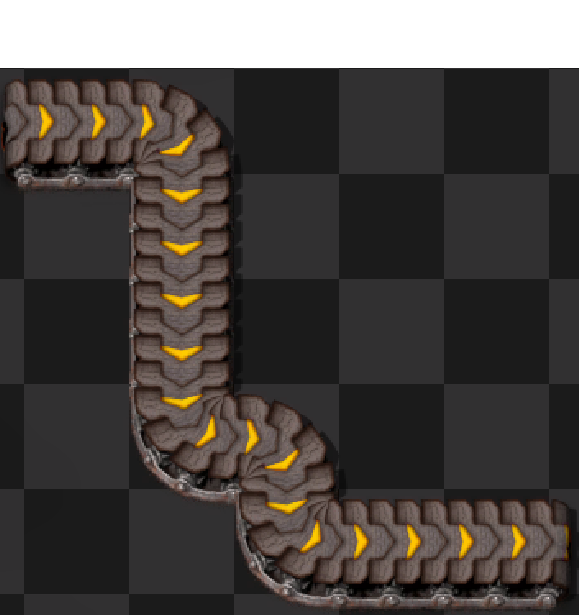
\includegraphics[width=0.9\linewidth]{Figures/captures_joc/exemples_model/5x5_route_instance.png}
        \caption{Representació gràfica de la variable \texttt{conveyor}}
    \end{subfigure}
    \hspace{1cm}
    \begin{subfigure}{.45\textwidth}
        \centering
        \newcolumntype{C}[1]{>{\centering\arraybackslash}m{#1}}
        \renewcommand{\arraystretch}{2.5} % Adjust the row height
        \begin{tabular}{|C{1cm}|C{1cm}|C{1cm}|C{1cm}|C{1cm}|}
            \hline
            1 & 6 & 0 & 0 & 0\\ \hline
            0 & 8 & 0 & 0 & 0\\ \hline
            0 & 13 & 0 & 0 & 0\\ \hline
            0 & 18 & 19 & 0 & 0\\ \hline
            0 & 0 & 21 & 22 & 23\\ \hline
        \end{tabular}
        \caption{Assignacions de la variable \texttt{route}}
    \end{subfigure}
    \caption{Exemple bàsic d'assignacions que compleixen amb les restriccions que defineixen una ruta}
\end{figure}



\begin{figure}[H]
    \centering
    \begin{subfigure}{.45\textwidth}
        \centering
        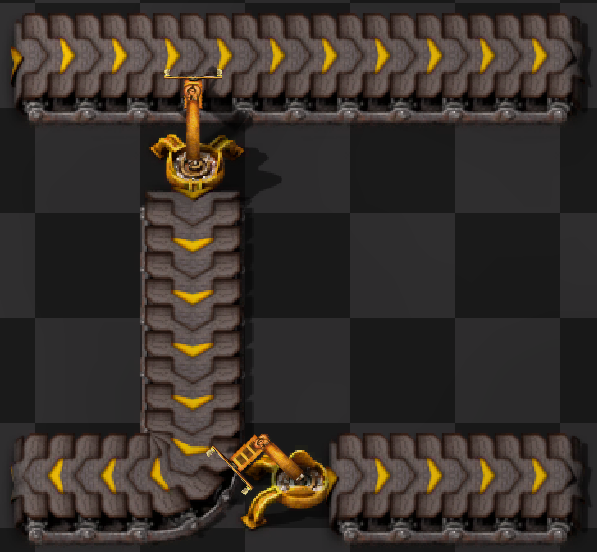
\includegraphics[width=0.9\linewidth]{Figures/captures_joc/exemples_model/5x5_instance_3_out.png}
        \caption{Representació gràfica de la variable \texttt{conveyor}}
    \end{subfigure}
    \hspace{1cm}
    \begin{subfigure}{.45\textwidth}
        \centering
        \newcolumntype{C}[1]{>{\centering\arraybackslash}m{#1}}
        \renewcommand{\arraystretch}{2.5} % Adjust the row height
        \begin{tabular}{|C{1cm}|C{1cm}|C{1cm}|C{1cm}|C{1cm}|}
            \hline
            1 & 2 & 22 & 23 & 24\\ \hline
            0 & 3 & 0 & 0 & 0\\ \hline
            0 & 4 & 0 & 0 & 0\\ \hline
            0 & 7 & 0 & 0 & 0\\ \hline
            14 & 12 & 15 & 20 & 23\\ \hline
        \end{tabular}
        \caption{Assignacions de la variable \texttt{route}}
    \end{subfigure}
    \caption{Exemple d'assignacions que compleixen amb les restriccions que defineixen una ruta, aquesta amb bifurcacions}
\end{figure}

\begin{figure}[h]
    \centering
    \begin{subfigure}{0.45\textwidth}
        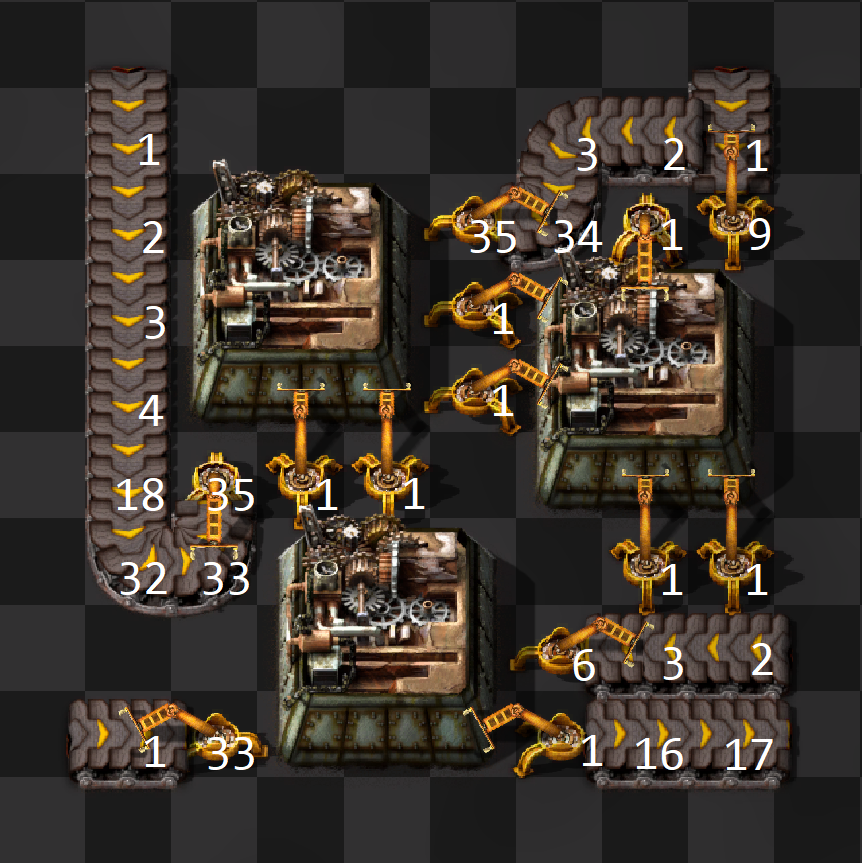
\includegraphics[width=\textwidth]{Figures/captures_joc/exemples_model/example_route_values.png}
        \caption{Variable \textit{route}}
    \end{subfigure}
    \hfill
    \begin{subfigure}{0.45\textwidth}
        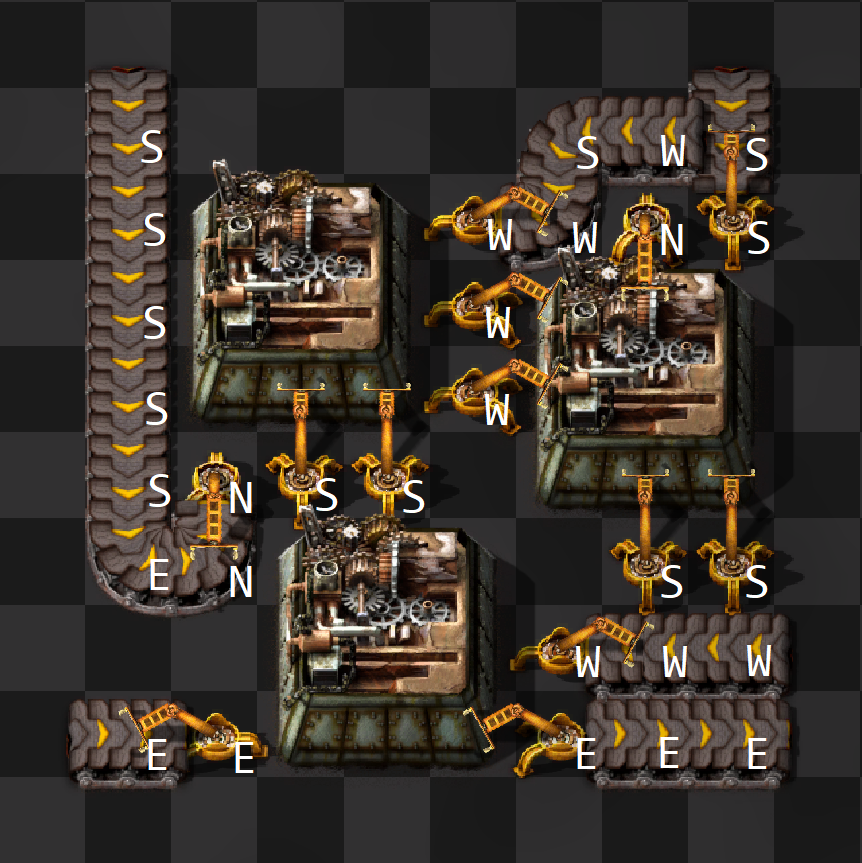
\includegraphics[width=\textwidth]{Figures/captures_joc/exemples_model/example_dir_values.png}
        \caption{Variable inseridor i cinta}
    \end{subfigure}
    \caption{Assignacions de les variables a l'exemple, les assignacions amb valor 0 o \textit{empty} s'han ignorat, les direccions de l'inseridor i \textit{conveyor} s'han posat en comú.}
\end{figure}



\subsection{Restriccions dels assembladors}
A l'hora de representar els assembladors hem de tenir en compte que ocupen un espai de 3x3 caselles, això complica la detecció de col·lisions entre ells i entre la resta d'objectes, així doncs, s'han usat dues variables per poder tenir control sobre la posició i àrea que ocupa cada assemblador. La primera variable \texttt{assembler} guarda la posició del centre de l'assemblador i tracta d'una matriu de mida $width-2 \times height-2$ amb domini $[0..(width/3)*(height/3)]$. El motiu pel qual la mida de la matriu no és la del \textit{blueprint} és perquè els assembladors en ocupar 3x3 caselles sabem que no hi ha cap assignació al perímetre exterior que sigui vàlida, així que ignorem aquestes posicions. La segona variable \texttt{collision} és una matriu de mida $width \times height$ i domini $[0..(width/3)*(height/3)]$. Aquesta variable guarda en quines posicions hi ha un assemblador, tot seguit les restriccions que en creen amb aquestes variables que ens permeten el control sobre les col·lisions.

\begin{table}[h]
    \centering
    \begin{tabular}{|c|c|c|}
    \hline
    \textbf{Variable} & \textbf{Mida} & \textbf{Domini} \\
    \hline
    assembler & $(width-2) \times (height-2)$ & $[0..(width/3)*(height/3)]$ \\
    \hline
    assembler\_collision & $width \times height$ & $[0..(width/3)*(height/3)]$ \\
    \hline
    \end{tabular}
    \caption{Variables implicades als assembladors}
    \label{assembler-variables}
\end{table}

\subsubsection{Col·lisió dels assembladors}
Aquesta restricció s'assegura que per cada posició de la matriu de la variable \texttt{assembler} on el valor sigui superior a 0 (és a dir que hi ha un assemblador), les 3x3 caselles adjacents a la matriu de la variable \texttt{collision} hagin de ser del mateix valor. D'aquesta manera ja tenim una variable on tenim representades les caselles on hi ha assembladors.
Amb aquesta restricció ja ens assegurem que no hi hagi col·lisions entre assembladors, ja que en cas que el \textit{solver} hagi assignat dos assembladors a posicions on intersequen, aquesta restricció farà que hi hagi caselles que han de prendre dos valors diferents, avaluant així a fals i sent necessari la reubicació de les posicions per evitar-ho.

\begin{lstlisting}[language=Python, caption=Assembler Collision]
for each cell (i, j) in the grid of size (height x width):
    surround_collision = []
    for each neighbor (di, dj) in the 3x3 grid centered at (i, j):
        x = di + i - 1
        y = dj + j - 1
        if 0 <= x < height and 0 <= y < width:
            surround_collision += collision_area[x][y] == assembler[i][j]
    assert Implies(assembler[i][j] != 0, And(surround_collision))
\end{lstlisting}
\begin{align*}
    &\forall i \in 0..width, \, \forall j \in 0..height, \\
    &assembler[i][j] != 0 \rightarrow \\
    &(collision\_area[i-1][j] == assembler[i][j] \land\\
    &collision\_area[i-1][j-1] == assembler[i][j] \land ...)
\end{align*}

Així i tot, amb això no n'hi ha prou, ja que no estem forçant a les caselles on no hi ha assembladors que prenguin el valor 0, impedint així la utilització d'aquesta variable per saber on hi ha exactament un assemblador.

\begin{figure}[H]
    \centering
    \begin{subfigure}{.45\textwidth}
        \centering
        \newcolumntype{C}[1]{>{\centering\arraybackslash}m{#1}}
        \renewcommand{\arraystretch}{2.5} % Adjust the row height
        \begin{tabular}{|C{1cm}|C{1cm}|C{1cm}|}
            \hline
            0 & 0 & 0\\ \hline
            0 & 0 & 0\\ \hline
            0 & 0 & 0\\ \hline
        \end{tabular}
        \caption{Variable \texttt{assembler} sense cap assemblador present}
    \end{subfigure}
    \hspace{1cm}
    \begin{subfigure}{.45\textwidth}
        \centering
        \newcolumntype{C}[1]{>{\centering\arraybackslash}m{#1}}
        \renewcommand{\arraystretch}{2.5} % Adjust the row height
        \begin{tabular}{|C{1cm}|C{1cm}|C{1cm}|C{1cm}|C{1cm}|}
            \hline
            0 & 0 & 0 & 0 & 0\\ \hline
            0 & 1 & 1 & 0 & 0\\ \hline
            1 & 0 & 0 & 0 & 0\\ \hline
            1 & 1 & 0 & 1 & 0\\ \hline
            0 & 0 & 1 & 0 & 0\\ \hline
        \end{tabular}
        \caption{Variable \texttt{collision} prenent valors $>$ 0 on no hi ha assembladors}
    \end{subfigure}
    \caption{Exemple de com hi ha assignacions vàlides que no representen les posicions on es troben els assembladors}
\end{figure}


\subsubsection{Enllaçar col·lisió amb assemblador}
Amb aquesta restricció hem d'aconseguir que \texttt{collision} només pregui valors $>$ 0 on hi ha un assemblador, per a fer-ho només cal assegurar que per cada posició de la matriu de la variable \texttt{collision} si hi ha una casella que ha pres valor $>$ 0 llavors una de les 8 caselles adjacents a la variable\texttt{assembler} ha de tenir un valor $>$ 0.

\begin{figure}[H]
    \centering
    \begin{subfigure}{.45\textwidth}
        \centering
        \newcolumntype{C}[1]{>{\centering\arraybackslash}m{#1}}
        \renewcommand{\arraystretch}{1.5} % Adjust the row height
        \begin{tabular}{|C{0.5cm}|C{0.5cm}|C{0.5cm}|C{0.5cm}|C{0.5cm}|C{0.5cm}|}
            \hline
            0 & 0 & 0 & 0 & 0 & 0\\ \hline
            0 & 0 & 0 & 0 & 0 & 0\\ \hline
            0 & 0 & 0 & 0 & 0 & 0\\ \hline
            0 & 1 & 0 & 0 & 0 & 4\\ \hline
            0 & 0 & 0 & 0 & 0 & 0\\ \hline
            0 & 0 & 0 & 0 & 0 & 0\\ \hline
        \end{tabular}
        \caption{Variable \texttt{assembler} amb 2 assignacions $>$ 0}
    \end{subfigure}
    \hspace{1cm}
    \begin{subfigure}{.45\textwidth}
        \centering
        \newcolumntype{C}[1]{>{\centering\arraybackslash}m{#1}}
        \renewcommand{\arraystretch}{1.5} % Adjust the row height
        \begin{tabular}{|C{0.5cm}|C{0.5cm}|C{0.5cm}|C{0.5cm}|C{0.5cm}|C{0.5cm}|C{0.5cm}|C{0.5cm}|}
            \hline
            0 & 0 & 0 & 0 & 0 & 0 & 0 & 0\\ \hline
            0 & 0 & 0 & 0 & 0 & 0 & 0 & 0\\ \hline
            0 & 0 & 0 & 0 & 0 & 0 & 0 & 0\\ \hline
            0 & 1 & 1 & 1 & 0 & 4 & 4 & 4\\ \hline
            0 & 1 & 1 & 1 & 0 & 4 & 4 & 4\\ \hline
            0 & 1 & 1 & 1 & 0 & 4 & 4 & 4\\ \hline
            0 & 0 & 0 & 0 & 0 & 0 & 0 & 0\\ \hline
            0 & 0 & 0 & 0 & 0 & 0 & 0 & 0\\ \hline
        \end{tabular}
        \caption{Variable \texttt{collision} prenent valors a l'àrea 3x3 només on hi ha presents assembladors}
    \end{subfigure}
    \caption{Exemple de com amb l'anterior restricció s'aconsegueix representar exactament la col·lisió dels assembladors}
\end{figure}

\begin{lstlisting}[language=Python, caption=Link Assembler Collision]
for each cell (i, j) in the grid of size (height x width):
    neighbors = []
    for each neighbor (di, dj) in the 3x3 grid centered at (i, j):
        x = di + i - 1
        y = dj + j - 1
        if 0 <= x < placement_height and 0 <= y < placement_width:
            neighbors += assembler[x][y] == collision_area[i][j]
    assert Implies(collision_area[i][j] != 0,
              Or(neighbors))

\end{lstlisting}
\begin{align*}
    &\forall i \in 0..width, \, \forall j \in 0..height, \\
    &collision\_area[i][j] != 0 \rightarrow \\
    &(assembler[i-1][j] == collision\_area[i][j] \lor \\
    &assembler[i-1][j-1] == collision\_area[i][j] \lor ...)
\end{align*}


\subsection{Tipus d'objectes}
Per modelar quin tipus d'objectes passen per cada casella s'ha usat la variable \texttt{item\_flow} que tracta d'una matriu de mida $width \times height$ amb domini $[0..max\_items]$. \texttt{max\_items} és un upper bound que es pot calcular a partir de les entrades del model, concretament donat l'ítem de sortida que el \textit{blueprint} ha de produir, podem analitzar quines receptes el produeixen i quins elements requereixen aquestes receptes així recursivament fins que només quedin objectes bàsics que no s'obtenen com a sortida d'una recepta.\\
Les restriccions associades al flux d'objectes són les següents:
\begin{table}[h]
    \centering
    \begin{tabular}{|c|c|c|}
    \hline
    \textbf{Variable} & \textbf{Mida} & \textbf{Domini} \\
    \hline
    item\_flow & $width \times height$ & $[0..max\_items]$ \\
    \hline
    \end{tabular}
    \caption{Variables implicades al tipus d'objectes}
    \label{item_flow-variables}
\end{table}

\subsubsection{Forma part de la ruta} \label{subsubsec:part_of_route_object_type}
Amb aquesta restricció fem que per totes les posicions \texttt{i j} de la variable \texttt{route} que prenguin un valor superior a 0, és a dir que formen part d'una ruta, forcen que a la mateixa posició \texttt{i j} de la variable \texttt{item\_flow} el valor pres sigui superior a 0, és a dir que transporten algun objecte.
\begin{lstlisting}[language=Python, caption=Part of Route]
for each cell (i, j) in the grid of size (height x width):
        assert (route[i][j] > 0) == (item_flow[i][j] > 0)
\end{lstlisting}
\begin{align*}
    &\forall i \in 0..width, \, \forall j \in 0..height, \\
    & route[i][j]>0 \leftrightarrow item\_flow[i][j]>0
\end{align*}


\subsubsection{Entrada i sortida d'objectes}
Com s'ha comentat a l'apartat \nameref{sec:blueprint_problem} una de les entrades del model tracta d'especificar quins objectes hi ha d'haver a les caselles d'entrada i sortida. Aquesta restricció, doncs, s'encarrega d'assegurar que aquestes caselles portin els objectes especificats.
\begin{lstlisting}[language=Python, caption=Item Input i Output]
for each cell (i, j) in input_cells:
    assert item_flow[i][j] == input_item(i, j)

for each cell (i, j) in output_cells:
    assert item_flow[i][j] == output_item(i, j)
\end{lstlisting}
\begin{align*}
    &\forall i \in 0..width, \, \forall j \in 0..height, \\
    & item\_flow[i][j] == input\_item(i, j)
\end{align*}
\begin{align*}
    &\forall i \in 0..width, \, \forall j \in 0..height, \\
    & item\_flow[i][j] == output\_item(i, j)
\end{align*}



\subsubsection{Propagació del tipus d'objectes}
Finalment, la restricció més important és la que s'encarrega d'assegurar que els objectes especificats a les entrades, sortides i els objectes requerits i produïts per les receptes associades al assembladors, es distribueixen correctament per les rutes.\\

Per aconseguir aquest comportament els que s'ha fet és, per totes les posicions del \textit{blueprint}, i cada posició ortogonalment veïna a la casella que estigui dins el \textit{blueprint}, si la casella té un valor a la variable $\texttt{route} > 0$, la direcció on es troba respecte a la direcció de la casella central és l'oposada i la casella central tracta d'un inseridor, llavors el valor de la variable \texttt{item\_flow} a la posició del inseridor ha de ser la mateixa que la de la posició veïna.\\
D'altra banda, i de manera molt similar si la casella ortogonalment veïna té un valor a la variable $\texttt{route} > 0$ i es troba en la mateixa direcció que l'inseridor central llavors és la casella veïna que ha de tenir el mateix valor a \texttt{item\_flow} que la casella central.\\
Finalment, si la casella central tracta d'una cinta, només cal assegurar que la casella veïna que es troba en la mateixa direcció que la cinta central ha de tenir el mateix valor a \texttt{item\_flow} que la cinta.\\

\begin{lstlisting}[language=Python, caption=Item Carry]
for each cell (i, j) in the grid of size (height x width):
    inserter_carry = []
    conveyor_carry = []
    for each dir in [north, east, south, west]:
        x = i + displacement[dir][0]
        y = j + displacement[dir][1]
        if 0 <= x < height and 0 <= y < width:
            if not is_input(i, j):
                inserter_carry += Implies(And(inserter[i][j] == opposite(dir),
                                              route[x][y] > 0),
                                          item_flow[i][j] == item_flow[x][y])
                inserter_carry += Implies(And(inserter[i][j] == dir,
                                              route[x][y] > 0),
                                          item_flow[x][y] == item_flow[i][j])
            if not is_output(i, j):
                conveyor_carry += Implies(conveyor[i][j] == dir,
                                          item_flow[x][y] == item_flow[i][j])
    assert Implies(inserter[i][j] != empty, And(inserter_carry))
    assert Implies(conveyor[i][j] != empty, And(conveyor_carry))
\end{lstlisting}
\begin{align*}
    &\forall i \in 0..width, \, \forall j \in 0..height, \\
    & ((inserter[i][j]==south \land route[i-1][j] > 0) \rightarrow item\_flow[i][j] == item\_flow[x][y]) \land \\
    & ((inserter[i][j]==north \land route[i-1][j] > 0) \rightarrow item\_flow[x][y] == item\_flow[i][j]) \land \\
    & (conveyor[i][j]==north \rightarrow item\_flow[x][y] == item\_flow[i][j])
\end{align*}

Alguns detalls importants sobre la restricció són:\\
Només cal tenir en compte que la casella veïna tingui un valor a la variable \texttt{item\_flow} > 0 \\ si la casella central tracta d'un inseridor, ja que són els únics elements d'una ruta que a la seva entrada o sortida hi pot haver un assemblador és a dir una posició on mai hi pot haver un valor d'$\texttt{item\_flow} > 0$.\\

Les caselles de sortida del \textit{blueprint}, que només poden ser cintes, no han de propagar el seu objecte, d'aquí la comprovació de \texttt{if not is\_output(i, j)}.\\

Tot i que no hi pot haver inseridors a les posicions d'entrada d'objectes, s'ha afegit la comprovació de \texttt{if not is\_input(i, j)}, ja que ens estalvia afegir restriccions addicionals.\\

Les implicacions finals són redundants, ja que només iterem per les direccions \texttt{[north, east, south, west]} i les implicacions anteriors asseguren que les direccions de les cintes i inseridors siguin la mateixa que iterem o l'oposada, les quals mai seran \texttt{empty}, així i tot, les implicacions finals ajuden a reduir el temps de solving, d'alguna manera deuen estar ajudant al solver a propagar més fàcilment les implicacions anteriors.

\subsection{Quantitat d'objectes}
Per determinar la quantitat d'objectes que passen per una casella, he decidit usar la mesura d'objectes per minut, el motiu és perquè té un bon balanç entre precisió i eficiència a l'hora de definir el domini de la variable.\\
Modelar aquesta mecànica del joc és de les més costoses i difícils de replicar, tot seguit explico les variables usades, el raonament els pros i contres.\\
Per cada casella cal saber quants objectes entren i quants surten, per poder modelar aquests objectes se sumen i reparteixen. Així doncs, s'han usat dues variables: \texttt{input\_flow\_rate} i \texttt{output\_flow\_rate} que són dues matrius de mida $width \times height$ i els seus dominis $[0..450]$ on 450 és el màxim nombre d'objectes per minut que un element de la ruta pot dur, en aquest cas la cinta, així que s'haurà d'anar amb compte i assegurar que els inseridors duguin més objectes per minut que la seva capacitat màxima de 50.\\
Les variables \texttt{output\_flow\_rate} i \texttt{input\_flow\_rate} són de tipus real, ja que les ràtios d'entrada/sortida de moltes receptes fan que una entrada entera d'objectes minut produeixi un nombre decimal d'objectes de sortida, i arrodonir aquests representa perdre molta precisió i allunyar-se dels casos reals que es podrien assolir amb les mecàniques originals del joc.

Les restriccions associades a aquestes variables que modelen la quantitat d'objectes que circulen pel \textit{blueprint} són les següents:
\begin{table}[h]
    \centering
    \begin{tabular}{|c|c|c|}
    \hline
    \textbf{Variable} & \textbf{Mida} & \textbf{Domini} \\
    \hline
    input\_flow\_rate & $width \times height$ & $[0..450]$ \\
    \hline
    output\_flow\_rate & $width \times height$ & $[0..450]$ \\
    \hline
    \end{tabular}
    \caption{Variables implicades a la quantitat d'objectes}
    \label{item_flow_rate-variables}
\end{table}


\subsubsection{Forma part de la ruta}
De manera molt similar a la restricció \nameref{subsubsec:part_of_route_object_type}, qualsevol posició \texttt{i j} del \textit{blueprint} que no formi part de la ruta no pot dur cap mena d'objecte i com a conseqüència el nombre d'objectes per minut que transporta ha de ser 0.

\begin{lstlisting}[language=Python, caption=Part of Route]
for each cell (i, j) in the grid of size (height x width):
    assert Implies(route[i][j] == 0, 
                   And(input_flow_rate[i][j] == 0,
                       output_flow_rate[i][j] == 0))
\end{lstlisting}
\begin{align*}
    &\forall i \in 0..width, \, \forall j \in 0..height, \\
    & route[i][j]==0 \rightarrow (input\_flow\_rate[i][j] == 0 \land output\_flow\_rate[i][j] == 0)
\end{align*}


\subsubsection{Quantitat d'entrada}
Una de les dades que tenim del \textit{blueprint} és la quantitat d'objectes per minut que hi ha a les caselles d'entrada, així que aquesta restricció assegura que el valor de la variable \texttt{input\_flow\_rate} a les posicions \texttt{i j} d'entrada, és l'especificada pel \textit{blueprint}.

\begin{lstlisting}[language=Python, caption=Item Input Rate]
for each cell (i, j) in input_cells:
    assert input_flow_rate[i][j] == input_rate[i][j]
\end{lstlisting}
\begin{align*}
    &\forall i \in 0..width, \, \forall j \in 0..height, \\
    & input\_flow\_rate[i][j] == input\_rate[i][j]
\end{align*}


\subsubsection{Propagació de la quantitat d'objectes (Cintes)}
La part més important de modelar la quantitat d'objectes que circulen per una cel·la que forma part de la ruta és definir quina serà l'entrada i sortida d'objectes en funció dels elements adjacents. Com el model consta de cintes i inseridors els quals tenen comportaments bastant diferents, la propagació de la quantitat d'objectes s'ha separat per cintes i inseridors.
Pel que fa a les cintes hi ha dues normes que defineixen com es distribueix la quantitat d'objectes:\\
Per cada posició \texttt{i j} del \textit{blueprint} on hi hagi una cinta, el valor de la variable \texttt{input\\\_flow\_rate} a la posició \texttt{i j} ha de ser la suma dels valors de la variable \texttt{output\\\_flow\_rate} a les posicions ortogonalment adjacents, les quals hi hagi un element de ruta, tant un inseridor com una altra cinta, on la seva direcció apunti a qualsevol de les 3 entrades de la cinta central. És a dir l'entrada d'una cinta és la suma de sortides dels elements de la ruta que aporten objectes a aquesta cinta.\\
Paral·lelament, per cada posició \texttt{i j} del \textit{blueprint} on hi hagi una cinta, el valor de la variable \texttt{output\_flow\_rate} a la posició \texttt{i j} serà el valor la variable \texttt{input\_flow\_rate} de la mateixa cinta, menys la suma de \texttt{input\_flow\_rate} d'inseridors a les posicions adjacents a la cinta, els quals treguin elements de la dita cinta, és a dir que la seva direcció sigui la mateixa a la direcció de la casella adjacent a la cinta central.\\
Tot seguit un exemple visual per entendre bé el que s'ha descrit.

\begin{lstlisting}[language=Python, caption=Belt Item Flow Propagation]
belt_flow_rate_propagation = []
for each cell (i, j) in the grid of size (height x width):
    belt_input = []
    belt_output = []
    for each dir in [north, east, south, west]:
        x = i + displacement[dir][0]
        y = j + displacement[dir][1]
            if 0 <= x < height and 0 <= y < width:
                belt_input += (If(And(conveyor[i][j] != dir,
                                            Or(conveyor[x][y] == opposite(dir),
                                               inserter[x][y] ==opposite(dir)),
                                            output_flow_rate[x][y], 0))
                                            
                belt_output += (If(inserter[x][y] == dir,
                                         input_flow_rate[x][y], 0))
    if not is_input(i, j):
        assert Implies(conveyor[i][j] != empty,
                        And(input_flow_rate[i][j] == sum(belt_input), input_flow_rate[i][j] <= 450))

    assert Implies(conveyor[i][j] != empty,
                   output_flow_rate[i][j] == 
                   (input_flow_rate[i][j] - sum(belt_output)))
\end{lstlisting}

\subsubsection{Propagació de la quantitat d'objectes (inseridors)}
Pel que fa als inseridors, la propagació de la quantitat d'objectes és lleugerament diferent de la de les cintes, ja que la seva capacitat de transport és de tan sols 50 objectes per minut. A banda la quantitat d'objectes que un inseridor agafa depèn de si l'inseridor està agafant objectes d'una cinta o si es tracta d'un inseridor de sortida d'un assemblador, així doncs es requereixen tres restriccions per modelar el comportament dels inseridors.\\

Per cada posició \texttt{i j} del \textit{blueprint} on hi hagi un inseridor, és a dir on la variable \texttt{inserter[i][j]$\neq$empty}, i per cada casella \texttt{x y} ortogonalment adjacent a l'inseridor, si la casella veïna està en la direcció oposada a l'inseridor i aquesta té un valor a la variable \texttt{input\_flow\_rate[x][y]$\ge50$}, llavors el valor d'entrada \texttt{input\_flow\_rate} i de sortida \texttt{output\_flow\_rate} l'inseridor haurà de ser 50, ja que un inseridor sempre que pugui agafarà el màxim d'objectes disponibles de la casella de la qual se supleix.\\

En cas que el valor de \texttt{input\_flow\_rate[x][y]$<50$} i el valor de ruta a la posició \texttt{route[x][y]$\neq0$}, significa que l'inseridor està prenent objectes d'una cinta la qual la seva entrada és inferior a 50 objectes minut, per tant, el valor d'entrada \texttt{input\_flow\_rate} i de sortida \texttt{output\_flow\_rate} l'inseridor haurà de ser igual que el valor d'entrada de la casella veïna.\\

Finalment, en cas que el valor de ruta a la casella veïna sigui \texttt{route[x][y]$=0$} significa que l'inseridor està traient objectes produïts per la recepta d'un assemblador, en aquest cas no es pot especificar la quantitat d'entrada o sortida de l'inseridor, així que només assegurem que el possible valor que la recepta de l'assemblador assigni a l'inseridor estigui dins el rang de transport, $0\ge$\texttt{input\_flow\_rate[i][j]}$\ge50$ i $0\ge$\texttt{output\_flow\_rate[i][j]}$\ge50$.

\begin{lstlisting}[language=Python, caption=Inserter Item Flow Propagation]
for each cell (i, j) in the grid of size (height x width):
    inserter_input = []
    for each dir in [north, east, south, west]:
        x = i + displacement[dir][0]
        y = j + displacement[dir][1]
            if 0 <= x < height and 0 <= y < width:
                inserter_input += Implies(And(inserter[i][j] == opposite(dir),
                                              input_flow_rate[x][y] >= 50),
                                          And(input_flow_rate[i][j] == 50,
                                              output_flow_rate[i][j] == 50))
                inserter_input += Implies(And(inserter[i][j] == opposite(dir),
                                              input_flow_rate[x][y] < 50,
                                              route[x][y] != 0),
                                          And(input_flow_rate[i][j] == input_flow_rate[x][y],
                                              output_flow_rate[i][j] == input_flow_rate[x][y]))
                inserter_input += Implies(And(inserter[i][j] == opposite(dir),
                                              route[x][y] == 0),
                                          And(input_flow_rate[i][j] == output_flow_rate[i][j],
                                              input_flow_rate[i][j]<=50,
                                              input_flow_rate[i][j]>=0,
                                              output_flow_rate[i][j]<=50,
                                              self.output_flow_rate[i][j]>=0))

        assert Implies(inserter[i][j] != empty, And(inserter_input))
\end{lstlisting}

\subsection{Receptes}
Juntament amb la quantitat d'objectes, les receptes són una de les parts més importants del model. Les receptes requereixen totes les anteriors restriccions descrites, ja que necessiten cert tipus d'objectes com a entrada, en funció de la quantitat en produeixen una quantitat de sortida, es produeixen en els assembladors i l'única manera de fer-los arribar és mitjançant rutes.\\

Per modelar les receptes, primer necessitem associar una recepta a un assemblador, això s'ha fet usant la variable \texttt{selected\_recipe}, aquesta variable tracta d'un array tipus BitVector, la seva mida és de \texttt{max\_assemblers} que com s'ha explicat anteriorment es calcula fent $(width/3) * (height/3)$. El domini de la variable és  $[0..\texttt{max\_recipes}]$, on \texttt{max\_recipes} tracta d'un upper bound que es calcula de manera molt similar a \texttt{max\_items}, donat l'objecte que es vol fabricar al \textit{blueprint} es pot saber quina recepta el fabrica i els objectes que necessita, recursivament podem saber quantes receptes pengen de la recepta que produeix la recepta final i establir l'upper bound.\\

Un cop podem saber quina recepta té associada cada assemblador, ens cal assegurar que a l'assemblador només entren i surten els objectes requerits per la recepta que té associada. Per definir aquest comportament no ha sigut necessària cap variable més així que tot seguit s'explicarà les restriccions associades i les variables implicades anteriorment descrites.\\

Finalment, hem d'assegurar que l'assemblador està produint la quantitat correcta d'objectes en funció de la recepta seleccionada i la quantitat d'objectes entrants. Aquesta és la part més complexa de les receptes, ja que els objectes poden entrar a l'assemblador en diferents ràtios i com ja s'ha explicat a l'apartat \nameref{subsec:recipes}, hi ha una quantitat màxima d'objectes entrants els quals la recepta pot processar.\\
La idea per modelar aquests comportaments ha sigut la següent:\\
Per decidir quina ha de ser la quantitat d'objectes de sortida, per cada assemblador ens cal saber les ràtios d'entrada de la recepta, aquesta informació la tindrem a la variable \texttt{input\_ratio} que tracta d'una matriu de mida \texttt{max\_assemblers}$\times$\texttt{max\_items}, de domini $[0..1]$ i de tipus Real.\\
Amb les ràtios de cada objecte d'entrada per cada assemblador, necessitem saber quina és la mínima ràtio per així saber quina és la quantitat d'objectes màxima que pot generar l'assemblador amb els ingredients d'entrada. Així doncs, la ràtio mínima es guarda en una variable auxiliar \texttt{min\_ratio} que tracta d'un array de mida \texttt{max\_assemblers}, de tipus Real i el seu domini igual que \texttt{input\_ratio} és $[0..1]$.\\

Amb les noves variables que formen part de les receptes, les restriccions que les utilitzen són les següents:

\begin{table}[h]
    \centering
    \begin{tabular}{|c|c|c|}
    \hline
    \textbf{Variable} & \textbf{Mida} & \textbf{Domini} \\
    \hline
    selected\_recipe & $1 \times max\_assemblers$ & $[0..max\_recipes]$ \\
    \hline
    input\_ratio & $max\_assemblers \times max\_items$ & $[0..1]$ \\
    \hline
    min\_ratio & $1 \times max\_assemblers$ & $[0..1]$ \\
    \hline
    \end{tabular}
    \caption{Variables implicades a les receptes}
    \label{recipe-variables}
\end{table}

\subsubsection{Associar recepta}
Amb aquesta restricció s'assegura que cada assemblador que formi part del \textit{blueprint} tingui una recepta associada, això es fa de la següent manera. Per cada assemblador \texttt{k} $[1..max\_assemblers]$ i cada posició \texttt{i j} on hi pot haver un assemblador (width-2 $\times$ height-2), es mira si la variable \texttt{assembler[i][j]}$=$\texttt{k}, i si per alguna de les posicions \texttt{i j} es dona tal condició llavors la variable \texttt{selected\_recipe[k]} ha de ser diferent de 0, és a dir té una recepta vàlida associada, d'altra banda, si no es troba cap posició \texttt{i j} on \texttt{assembler[i][j]}$=$\texttt{k} llavors la variable \texttt{selected\_recipe[k]} ha de ser 0, és a dir que no té cap recepta associada.

\begin{lstlisting}[language=Python, caption=Associate Recipe]
for k in [1..max_assemblers]
    exists_assembler = []
    for each cell (i, j) in the grid of size (height-2 x width-2):
        exists_assembler += assembler[i][j] == k
    assert If(Or(exists_assembler),
              selected_recipe[k - 1] != 0,
              selected_recipe[k - 1] == 0)
\end{lstlisting}
\begin{align*}
    &\forall k in 0..max\_assemblers, \,  \forall i \in 0..width, \, \forall j \in 0..height, \\
    & input\_flow\_rate[i][j] \leftrightarrow input\_rate[i][j]
\end{align*}

\subsubsection{Ingredients d'entrada i sortida}
Per la recepta associada a un assemblador hem d'assegurar que els objectes que entren només siguin els que formen part dels ingredients d'entrada de la recepta. Per assegurar aquest comportament cal:
Per cada assemblador del \textit{blueprint} i cada inseridor amb direcció apuntant a l'assemblador, hem d'assegurar que com a mínim hi ha un inseridor per cada tipus d'objecte que la recepta requereix i que no hi ha cap inseridor que dugui un objecte no requerit per la recepta.\\
De la mateixa manera hem d'assegurar que hi hagi com a mínim un inseridor que s'endugui l'objecte que la recepta produeix.

\begin{lstlisting}[language=Python, caption=Assembler Input]
for each cell (i, j) in the grid of size (height-2 x width-2):
    for k in [1..max_assemblers]:
        assembler_selected = assembler[i][j] == k
        for item in [1..max_items]:
            inputs = []
            for dir in displacement:
                for pos in displacement[dir]:
                    x = i + 1 + pos[0]
                    y = j + 1 + pos[1]
                    if 0 <= x < height and 0 <= y < width:
                        inputs += And(inserter[x][y] == opposite(dir),
                                          item_flow[x][y] == item)
            for recipe in [1..max_recipes]:
                recipe_selected = selected_recipe[k] == recipe
                if recipe_input[recipe][item] != 0:
                    assert Implies(And(assembler_selected, recipe_selected),
                           Or(inputs))
                else:
                    assert Implies(And(assembler_selected, recipe_selected),
                           Not(Or(inputs)))
\end{lstlisting}

\begin{lstlisting}[language=Python, caption=Assembler Output]
for each cell (i, j) in the grid of size (height-2 x width-2):
    for k in [1..max_assemblers]:
        assembler_selected = assembler[i][j] == k
        for item in [1..max_items]:
            outputs = []
            for dir in displacement:
                for pos in displacement[dir]:
                    x = i + 1 + pos[0]
                    y = j + 1 + pos[1]
                    if 0 <= x < height and 0 <= y < width:
                        outputs += And(inserter[x][y] == dir,
                                          item_flow[x][y] == item)
            for recipe in [1..max_recipes]:
                recipe_selected = selected_recipe[k] == recipe
                if recipe_output[recipe][item] != 0:
                    assert Implies(And(assembler_selected, recipe_selected),
                           Or(outputs))
                else:
                    assert Implies(And(assembler_selected, recipe_selected),
                           Not(Or(outputs)))
\end{lstlisting}

Alguns detalls importants de les restriccions són, primer \texttt{discplacement} tracta d'un diccionari Python amb quatre entrades representant cada direcció cardinal numerada de [1..4] i per cada direcció hi ha una llista amb les parelles de coordenades \texttt{x y} representant totes les caselles relatives a (0,0) que es consideren vàlides com a casella d'entrada o sortida d'un assemblador.\\
Segon, tot i que Z3 permet usar Arrays indexables per valors de variables enteres, aquests introdueixen noves teories al model que alenteixen el temps de solving, per això aquesta restricció ha d'iterar per cada assemblador, recepta i objecte. I usar dues variables auxiliars (\texttt{assembler\_selected}, \texttt{recipe\_selected}) per saber si l'assemblador que estem iterant tracta del assemblador a la posició \texttt{i j} i si la recepta que té associada tracta de la recepta que estem iterant.\\
Per últim, \texttt{recipe\_input} i \texttt{recipe\_output} són dues matrius Python que s'obtenen del preprocès de les entrades del \textit{blueprint}, concretament cada fila representa una recepta, cada columna un objecte i cada posició conté quants objectes per minut usa aquella recepta en cas de \texttt{recipe\_input} i quants objectes produeix en cas de \texttt{recipe\_output}.

\subsubsection{Ràtios d'entrada}
Com s'ha comentat anteriorment per determinar quants objectes ha de produir una recepta necessitem saber les ràtios dels objectes d'entrada, aquesta restricció s'encarrega justament d'això.\\
La implementació és molt similar a les restriccions d'ingredients d'entrada i sortida, per cada assemblador a la posició \texttt{i j} del \textit{blueprint} i cada posició veïna vàlida per l'entrada d'objectes mitjançant inseridors, ens guardem la suma de \texttt{output\_flow\_rate[i][j]} dels inseridors que portin el mateix tipus d'objecte, gràcies al fet que la restricció anterior ens assegura que només hi hagi inseridors afegint objectes que formen part de la recepta, no cal comprovar el tipus d'objecte que transporta l'inseridor, només la quantitat. Aquesta suma l'hem de dividir pel màxim nombre d'objectes que la recepta accepta d'aquell tipus (\texttt{recipe\_input[recepta][objecte]}) obtenint així la ràtio d'entrada de cada objecte, aquesta ràtio la guardem a la variable \texttt{input\_ratio[assembler][objecte]}.

\begin{lstlisting}[language=Python, caption=Input Ratio]
for each cell (i, j) in the grid of size (height-2 x width-2):
    for k in [1..max_assemblers]:
        assembler_selected = assembler[i][j] == k
        for item in [1..max_items]:
            inputs = []
            for dir in displacement:
                for pos in displacement[dir]:
                    x = i + 1 + pos[0]
                    y = j + 1 + pos[1]
                    if 0 <= x < height and 0 <= y < width:
                        inputs += If(And(inserter[x][y] == opposite(dir),
                                         item_flow[x][y] == item),
                                     output_flow_rate[x][y], 0)
            for recipe in [1..max_recipes]:
                recipe_selected = selected_recipe[k] == recipe
                if recipe_input[recipe][item] != 0:
                    assert Implies(And(assembler_selected,
                                       recipe_selected),
                                   input_ratio[k][item] == 
                                   sum(inputs)/recipe_input[recipe][item])
                else:
                    assert Implies(And(assembler_selected,
                                       recipe_selected),
                                   input_ratio[k][item] == 1)
\end{lstlisting}

Un detall important de la implementació és que quan un objecte no s'usa com a ingredient en una recepta, el valor de la seva ràtio es posa a 1, això és important, ja que per la següent restricció ens serà molt útil.

\subsubsection{Ràtio mínima}
Amb les ràtios de cada objecte per cada assemblador, només ens queda saber quin és el mínim, això s'aconsegueix usant la variable auxiliar \texttt{min\_ratio} anteriorment descrita. Per forcar que el valor que prengui la variable \texttt{min\_ratio} sigui el mínim de cada objecte del assemblador, és molt simple, per cada assemblador \texttt{k} i cada objecte \texttt{i}, cal que el valor de \texttt{min\_ratio[k]} sigui un valor de qualsevol objecte de la variable que aparegui \texttt{input\_ratio[k]} i a més també cal forçar que el valor de \texttt{min\_ratio[k]} sigui més petit igual a tots els valors dels objectes de \texttt{input\_ratio[k]}. D'aquesta manera al valor haurà de ser el més petit i formar part dels possibles valors de les ràtios.

\begin{lstlisting}[language=Python, caption=Min Ratio]
for k in [1..max_assemblers]:
    value_of = []
    min_value = []
    for item in [1..max_items]:
        value_of += min_ratio[k] == input_ratio[k][item]
        min_value += min_ratio[k] <= input_ratio[k][item]
    assert Or(value_of)
    assert And(min_value)
\end{lstlisting}

\subsubsection{Quantitat d'objectes de sortida}
Amb totes les peces del puzle llestes, només cal definir quants objectes per minut ha de produir la recepta associada al assemblador.\\
De manera similar a anteriors restriccions, per cada assemblador del \textit{blueprint} i per cada posició vàlida d'entrada i sortida d'objectes del assemblador sumem el nombre d'objectes per minut que els inseridors estan extraient. Aquesta suma ha de ser igual al valor de la variable \texttt{min\_ratio} a la columna del assemblador que estiguem mirant multiplicat pel màxim teòric que pot produir la recepta \texttt{recipe\_output[recepta][objecte]}.

\begin{lstlisting}[language=Python, caption=Min Ratio]
for each cell (i, j) in the grid of size (height-2 x width-2):
    for k in [1..max_assemblers]:
        assembler_selected = assembler[i][j] == k + 1
        outputs = []
        for dir in displacement:
            for pos in displacement[dir]:
                x = i + 1 + pos[0]
                y = j + 1 + pos[1]
                if 0 <= x < height and 0 <= y < width:
                    outputs += If(inserter[x][y] == dir,
                                  output_flow_rate[x][y],
                                  0))
        for recipe in [1..max_recipes]:
            recipe_selected = selected_recipe[k] == recipe + 1
            for item in [1..max_items]:
                if recipe_output[recipe][item] != 0:
                    assert Implies(And(assembler_selected,
                                       recipe_selected),
                                   sum(outputs) == min_ratio[assembler] * recipe_output[recipe][item])
\end{lstlisting}


\section{Canvis fets al model per aproximar-lo més al comportament real del joc}\label{mecanics-changes}

La primera iteració del model és completament funcional, però hi ha alguns comportaments que no acaben de ser com al Factorio. Tot seguit s'explica quins d'aquests comportaments es poden extrapolar del joc al model i quins requeririen massa complexitat i s'han deixat de banda.

\subsection{Propagació de la quantitat d'objectes en inseridors}

Com s'ha explicat a l'apartat de la implementació d'aquesta mecànica, els inseridors sempre intenten transportar el màxim d'objectes possible, però amb la representació d'aquest comportament a l'anterior restricció, els inseridors només podrien prendre dos valors:\\
En cas que la sortida de la cinta de la qual agafen objectes fos superior a 50 aquests agafaven els 50 objectes/min, i en cas que l'output de la cinta fos inferior a 50 objectes per minut, l'inseridor agafa la quantitat de sortida de la cinta, definint d'aquesta manera el comportament de "sempre agafar el màxim possible". Però això no sempre és cert per dos motius:\\

Primer hi ha el cas que si l'inseridor deixa els objectes en una altra cinta i aquesta porta una quantitat d'objectes que en afegir-se els que l'inseridor porta se superi la capacitat de 450 objectes per segon, l'inseridor hauria de deixar la diferència d'objectes fent així que el seu output no fos el màxim que pot agafar de la cinta d'entrada.\\
Segon si un inseridor porta objectes a un assemblador i aquest no els necessita tots degut a que per la falta de quantitat d'un altre objecte no els pot processar, l'inseridor acabarà reduint la quantitat d'objectes que pot aportar a l'assemblador fins que porti exactament la mateixa quantitat d'objectes que l'objecte de la recepta de l'assemblador que fa de coll d'ampolla, fent així que la seva quantitat de sortida no sigui la mateixa que la màxima que pot agafar de la cinta d'entrada.\\

Per poder recrear el comportament real s'ha optat per fer el següent:\\
En comptes de fixar el seu input a 50 objectes/min si sortida de la cinta és més gran o igual a 50, ara si la sortida de la cinta és més gran o igual a 50 llavors l'entrada de l'inseridor haurà de ser com a molt 50 i com a molt poc més gran que 0, ja que si un inseridor no transporta objectes és inútil.\\
D'altra banda, l'output de la cinta d'entrada de l'inseridor és més petit que 50 objectes per minut, llavors l'input de l'inseridor podrà ser com a màxim la quantitat de sortida de la cinta.\\
És important tenir en compte que aquesta nova manera de representar els objectes que poden transportar els inseridors només representa en comportament real del joc, sempre que el criteri d'optimització sigui maximitzar la quantitat d'objectes que es volen produir, ja que si simplement volguéssim trobar una assignació que satisfés a totes les restriccions, ens podríem trobar casos on un inseridor dins el llindar que s'ha establert a la nova restricció, no fos el màxim. Però com l'objectiu del model és maximitzar la sortida i aquest no té gaire sentit sense aquest criteri d'optimització, aquesta nova implementació s'ha considerat completament vàlida i funcional.\\

Arran d'aquest canvi, hi ha una altra part de les restriccions que també requereix un canvi, tot seguit s'explica a la següent secció.

\subsection{Ràtios d'entrada i ràtio mínima}
A la primera iteració del model es va explicar que per poder calcular la quantitat d'objectes que un assemblador ha de produir, calia prendre com a referència l'objecte que en relació amb la quantitat que necessita la recepta està sent el menys suplit pels inseridors d'entrada. Però hi ha una part d'aquesta implementació que no s'ajusta del tot a com funciona el joc, principalment es deu al fet que si hi ha un objecte que en funció de la seva necessitat a la recepta s'està suplint amb major quantitat que un altre, aquest acaba saturant a l'assemblador fent que aquest al final només pugui processar la proporció relativa marcada per l'objecte que menys s'està suplint, és a dir si el model permet suplir més objectes dels que l'assemblador pot processar aquests s'haurien d'acumular a la cinta que supleix a l'inseridor de l'objecte esmentat, però amb l'antiga implementació aquest excés d'objectes simplement es volatilitzava pel fet que el que es feia era agafar la ràtio mínim d'entrada de l'assemblador per calcular la quantitat de sortida.\\
Arreglar aquest comportament no ha estat gaire difícil i a més en certa manera ha ajudat al model a causa de l'eliminació de la variable \texttt{min\_ratio}. El que s'ha fet és que com l'objecte que menys se supleix dictamina la quantitat dels altres objectes que l'assemblador podrà processar, simplement s'ha eliminat la variable \texttt{min\_ratio} i s'ha forçat que per cada objecte \texttt{k} a la variable \texttt{input\_ratio[k]} els seus valors siguin iguals, d'aquesta manera cada inseridor només podrà suplir a l'assemblador la quantitat d'objectes que fa que la seva ràtio d'entrada sigui igual que la resta, fent així que no hi hagi objectes que es perdin.\\

La nova restricció que iguala els valors de les ràtios per cada assemblador és la següent:

\begin{lstlisting}[language=Python, caption=Equal Ratios]
def equal_ratios(self):
    equal_ratios = []
    for j in range(self.max_assemblers):
        for i in range(1, self.max_items):
            equal_ratios.append(
            self.input_ratio[j][i] == self.input_ratio[j][0]
            )
    return equal_ratios
\end{lstlisting}

\subsection{Quantitat d’objectes de sortida}
Finalment, l'últim comportament del joc que la primera iteració del model no replica, tracta de la quantitat d'objectes que han de treure els inseridors d'un assemblador. El primer model simplement assegura que la suma d'objectes que treuen els inseridors de sortida siguin exactament la quantitat que l'assemblador produeix, però no diu res de quants objectes ha de treure cada inseridor. Això és un problema, ja que al joc si hi ha més d'un inseridor que treu objectes d'un assemblador la quantitat que aquest transporta ha de ser igual a la resta, així doncs el que s'ha fet és afegir una variable auxiliar a la restricció anterior que serveix perquè tots els inseridors que treuen objectes de l'assemblador tinguin el mateix valor, d'aquesta manera igualant la variable \texttt{output\_flow\_rate} a la posició \texttt{x}, \texttt{y} on es troba l'inseridor a la variable s'assegura que tots els inseridors que treuen objectes d'aquell assemblador transportin la mateixa quantitat d'objectes mantenint la propietat d'assegurar que la suma d'objectes dels inseridors sigui exactament igual a la produïda per l'assemblador.\\

L'antiga restricció amb el canvi aplicat queda de la següent manera:

\begin{lstlisting}[language=Python, caption=Output Rate]
def set_output_rate():
    output_ratios = []
    for i in range(placement_height):
        for j in range(placement_width):
            for assembler in range(max_assemblers):
                outputs = []
                output_rate = Real(f'output_rate_{i}_{j}_{assembler}')
                output_ratios.append(And(output_rate >= 0, output_rate <= 50))
                for direction in displacement:
                    for pos in displacement[direction]:
                        x = i + 1 + pos[0]
                        y = j + 1 + pos[1]
                        if 0 <= x < height and 0 <= y < width:
                            outputs.append(
                                If(inserter[x][y] == direction[direction], output_flow_rate[x][y],
                                   0))
                            output_ratios.append(Implies(self.inserter[x][y] == direction[direction],
                                                         output_flow_rate[x][y] == output_rate))
                first_item_ratio = next(iter(input_ratio[assembler + 1].values()))
                for output in recipes[selected_recipe[assembler]]["OUT"]:
                    output_ratios.append(Implies(assembler[i][j] == assembler + 1,
                                                 sum(outputs) == first_item_ratio * output[1]))
    return output_ratios
\end{lstlisting}

\section{Millores al model}
\subsection{Upper bound}\label{upper-bound}
Amb les mecàniques del joc replicades el millor possible al model, hi ha certes millores que es poden fer. La més simple tracta d'acotar el domini $[0..width * height]$ de la variable \texttt{route}, ja que si al blueprint no només hi ha cintes i inseridors sinó que també necessitem assembladors els quals ocupen 3x3 caselles, així que el domini de \texttt{route} es pot reduir sabent el nombre de receptes \texttt{max\_recipes} que implica crear un objecte determinat, com s'ha explicat anteriorment aquest valor es precalcula i és fàcil d'obtenir, finalment el nou domini de la variable serà $[0..width * height - max\_recipes * 9]$.

\subsection{Lower bound}\label{lower-bound}
Usant la mateixa idea d'abans, com se sap que la quantitat mínima d'assembladors que es necessitaran és igual al nombre de receptes diferents \texttt{max\_recipes}, podem crear una restricció que aprofiti aquesta informació i obligui que el nombre mínim d'assembladors presents al blueprint sigui \texttt{max\_recipes}.\\
La implementació és molt senzilla i només cal que per cada posició \texttt{i j} de la variable \texttt{assembler} i assegurar que la suma de posicions on el valor d'assemblador és superior a 0, és a dir hi ha un assemblador, sigui com a mínim \texttt{max\_recipes}.

\begin{lstlisting}[language=Python, caption=Lower Bound]
    def lower_bound_assemblers(self):
        lower_bound = []
        for i in range(self.placement_height):
            for j in range(self.placement_width):
                lower_bound.append(If(UGT(self.assembler[i][j], 0), 1, 0))
        return [sum(lower_bound) >= self.max_recipes]
\end{lstlisting}

\subsection{Pre computar les receptes associades als assemblers}\label{precompute-recipes}
Un dels inconvenients del model actual és que per saber quina recepta té associada cada assembler ens cal una variable nova la qual incorpora moltes simetries, ja que dos assemblers diferents amb receptes diferents es poden canviar de posició i canviar de recepta i obtenir el mateix resultat, és a dir si l'assembler 1 usa la recepta 2 a la posició (1, 1), i l'assembler 2 usa la recepta 1 a la posició (2, 2), és el mateix que si l'assembler 2 usa la recepta 2 a la posició (1, 1) i l'assembler 1 usa la recepta 1 a la posició (2, 2). El mateix passa si dos o més assemblers usen la mateixa recepta, aquests es poden permutar entre ells sense alterar el resultat.\\

La solució que s'ha proposat a aquest problema és bastant més complexa que les anteriors, ja que d'alguna manera cal saber quines receptes ha d'usar cada assembler abans d'inicial el procés de solving, aquest problema no és gens trivial i s'ha optat per generar un sistema d'equacions el qual s'ha de resoldre maximitzant la variable que representa l'objecte de sortida. Tot seguit el desenvolupament d'un exemple per entendre correctament el sistema d'equacions.\\

\subsubsection{Objectes i receptes}
Suposem que l'objecte que es vol produir tracta de circuits avançats, aquest objecte requereix la recepta Advanced-Circuit per ser produït. A partir d'aquesta recepta necessitem saber quins objectes necessita per ser fabricat que no siguin matèries primeres és a dir objectes que requereixen altres receptes per ser produïts. Concretament, necessita 40 cable de coure/min i 20 circuits electrònics/min així que aquests objectes impliquen les receptes de Copper-Cable el qual es pot produir íntegrament a partir de matèries primeres i circuit electrònic, que requereix 360 cable de coure per minut.\\

Així doncs, el desglossament de dependències de l'objecte circuit avançat en objectes és el següent:\\

\begin{tabular}{|c|c|c|}
\hline
\textbf{Recepta} & \textbf{Requereix} & \textbf{Produeix} \\ \hline

Circuit Avançat & 
\begin{tabular}{@{}c@{}}
40 Cable de Coure \\ \hline
20 Circuit Electrònic
\end{tabular} &  \\ \hline

Circuit Electrònic & 360 Cable de Coure & 120 Circuit Electrònic \\ \hline

Cable de Coure &  & 240 Cable de Coure \\ \hline
\end{tabular}

\subsubsection{Sistema d'equacions}

Amb aquesta informació podem construir un sistema d'equacions creant una variable real per cada recepta, aquesta variable representarà el percentatge d'assembladors que l'estan produint, és a dir 1 significa que hi ha un assemblador funcionant al 100\% i si és 1.2 significa que hi ha un assemblador funcionant al 100\% i un altre al 20\%, ja que un assemblador com a molt pot treballar al 100\% de la seva capacitat.\\
Per aquest exemple tindrem tres variables \texttt{cca}, \texttt{eca} i \texttt{aca}.\\

\begin{equation*}
\begin{cases}
240cca = 40aca+360eca\\
120eca = 20aca
\end{cases}
\end{equation*}
\\

Amb aquest sistema d'equacions es representa a la part esquerra els objectes que produeix la recepta en funció de la variable que indica la quantitat d'assembladors que la produeixen i a la part dreta la quantitat d'objectes que es necessiten en funció de la variable dels assembladors que necessiten l'objecte. D'aquesta manera s'assegura que per cada percentatge d'assembladors que produeixen una recepta hi ha exactament el nombre d'assembladors necessaris per poder abastir-lo.\\

\subsubsection{Limitar l'espai de solucions}
A banda del sistema d'equacions hem de delimitar quin és el nombre màxim d'assembladors que es poden usar, al cas del problema del \textit{blueprint} serà el nombre màxim d'assembladors que es poden encabir en les dimensions del blueprint $(width/3) * (height/3)$, en aquest exemple concret $\texttt{max\_assemblers} = 9$. El problema que sorgeix amb la representació actual és que no tenim cap manera de determinar quin és el nombre d'assembladors individuals que s'utilitzen, ja que les variables \texttt{cca}, \texttt{eca} i \texttt{aca} són reals i si les sumem no obtenim el nombre d'assembladors, per això cal obtenir el ceil de cada variable real per poder imposar que la suma d'assembladors no pugui superar el nombre màxim de \texttt{max\_assemblers}. El ceil de cada variable real es pot obtenir de dues maneres, la primera és una implementació que va molt lligada al funcionament del Z3 i la segona tracta d'una definició més formal del que significa el ceil.\\

La primera manera d'obtenir el ceil d'una variable real tracta de crear una variable auxiliar entera per cada variable real i definir una restricció que asseguri que l'únic valor que pot prendre la variable sigui el resultat d'aplicar el ceil a la variable real. Per a fer-ho es farà ús de la funció \texttt{ToInt()} del Z3 que rep per paràmetre la variable real i en retorna el valor enter, es a dir aplica un floor. Amb aquesta funció i la següent restricció podem definir el ceil:

\begin{lstlisting}[language=Python, caption=Ceil implementation 1]
s = Solver()
x = Real("x")
x_ceil = Int("x_ceil")
s.add(If(ToInt(x)<x, x_ceil==ToInt(x) + 1, x_ceil==ToInt(x)))
\end{lstlisting}

D'aquesta manera si el floor de la variable és més petit que el seu valor real significa que el seu ceil és el valor enter + 1 i en cas que el floor de la variable entera sigui igual que el valor real llavors el valor enter és el mateix que el valor real. Clarament, no cal tenir en compte el cas que el floor sigui més gran, ja que el floor d'un nombre decimal mai pot ser més gran que el mateix valor decimal.\\

Una altra manera d'obtenir el ceil d'una variable real tracta d'igual manera que amb l'anterior mètode crear una variable entera per cada real i definir una restricció on el valor que prengui la variable entera ha de ser més gran o igual a la real, ja que el ceil ha de ser un valor més gran en cas que la variable real tingui part decimal o el mateix valor en cas que la variable real no tingui pare decimal. A banda per assegurar que el valor que prengui la variable entera no sigui més gran que el ceil de la variable real s'afegeix la restricció que fa que el valor de la variable entera menys 1 ha de ser més petit que el valor de la variable real d'aquesta manera si el valor enter és superior al ceil aquesta restricció no se satisfarà.

\begin{lstlisting}[language=Python, caption=Ceil implementation 2]
s = Solver()
x = Real("x")
x_ceil = Int("x_ceil")
s.add(x_ceil-1<x)
s.add(x<=x_ceil)
\end{lstlisting}

Amb les variables que representen el ceil de cada variable només cal crear una restricció que asseguri que el nombre d'assembladors usats no superi el nombre màxim:

\begin{lstlisting}[language=Python, caption=Limit assemblers]
s.add(ceil_cca+ceil_eca+ceil_aca<=9)
\end{lstlisting}

\subsubsection{Optimització}
Sense criteri d'optimització el solver trobarà qualsevol assignació que compleixi les restriccions imposades, però això no és el que volem, el nostre objectiu és saber quina recepta ha de tenir associada cada assemblador tenint en compte que volem maximitzar la producció de l'objecte de sortida a l'entrada del model. Aquest pas va dur alguns problemes a l'hora de desenvolupar-lo, ja que l'optimitzador de Z3 permet maximitzar variables reals, la qual cosa pot semblar una tasca impossible perquè una variable real té infinites parts decimals dins un domini definit així que quan es va intentar optimitzar hi havia solucions subòptimes. Al final el que  maximitzar la part entera més la part decimal, ja que si només tenim en compte la part entera hi ha múltiples assignacions a la part decimal que donen al mateix resultat a la part entera que podrien desencadenar en què les receptes de les quals depèn l'objecte objectiu no funcionessin al màxim rendiment.

\begin{lstlisting}[language=Python, caption=Optimization]
s.maximize(aca_ceil + aca)
\end{lstlisting}

I la solució final és \texttt{[aca\_ceil = 5, eca\_ceil = 1, cca\_ceil = 3]} i \texttt{[aca = 5, eca = 5/6, cca = 25/12]}, així que ja sabem que per un blueprint on entren 9 assembladors i es vol produir circuits avançats, com a molt es necessitaran 5 assembladors dedicats a fabricar circuits avançats, 3 a fabricar copper cable i 1 dedicat a circuits electrònics.

\subsection{Eliminació de simetries}
Tot i que l'optimització anterior elimina les simetries on dos o més assembladors amb diferents receptes associades es poden permutar obtenint el mateix resultat, en cas que la recepta sigui la mateixa la simetria persisteix.\\

Per eliminar-la hem d'imposar ordre entre els assembladors que comparteixen la mateixa recepta d'aquesta manera les assignacions que siguin simètriques entre elles només seran satisfacibles si els assembladors tenen cert ordre.\\
La implementació actual no permet ordenar directament les posicions dels assembladors, ja que aquests no tenen una variable posició. Per poder ordenar-los s'han creat dues variables auxiliars \texttt{x} amb domini $[0..height]$ i \texttt{y} amb domini $[0..width]$ per tots els assembladors que comparteixen la mateixa recepta, això ho podem fer gràcies a l'optimització anterior que precalcula quina recepta ha de produir cada assemblador.\\
Amb aquesta variable no és suficient, ja que d'alguna manera hem d'enllaçar les posicions ordenades amb la variable \texttt{assembler}, aquí sorgeix un altre problema, ja que el pre càlcul de les receptes calcula el màxim d'assembladors de cada recepta que es podrien arribar a usar, però no tenen per què usar-se tots, així que d'alguna manera cal assegurar-se que es faci l'ordenació de posicions i l'enllaç amb una quantitat no fixada d'assembladors. Per resoldre aquest problema s'ha afegit una tercera variable booleana \texttt{used} que indica si l'assemblador s'està usant. D'aquesta manera amb una simple implicació lògica es pot forçar que només els assembladors en ús s'enllacin i s'ordenin.\\

Les restriccions que asseguren l'ordenació i l'enllaç són força simples. Per l'ordenació només cal que per cada parella de posicions $x_1 x_2$ i $y_1 y_2$ dels assembladors que comparteixin la mateixa recepta la posició $x_1 \leq x_2$ ja que en tractar-se d'un tauler 2D és possible que les coordenades $x$ coincideixin, en aquest cas també cal assegurar que $y_1 < y_2$, per les coordenades $y$ no cal tenir en compte el cas en què siguin iguals, ja que això significaria que els dos assembladors se superposen, cosa que mai pot passar.

\begin{lstlisting}[language=Python, caption=Posicions ordenades]
for recipe in assembler_recipes:
    assemblers = assembler_recipes[recipe]
    assembler_keys = list(assemblers.keys())
    for i in range(len(assembler_keys) - 1):
        x0, y0, used0 = assemblers[assembler_keys[i]]
        x1, y1, used1 = assemblers[assembler_keys[i + 1]]
        symmetry_breaking.append(UGE(used0, used1))
        symmetry_breaking.append(Implies(And(used0 == 1, used1 == 1), And(ULE(x0, x1), Implies(x0 == x1, ULT(y0, y1)))))
\end{lstlisting}

En aquest fragment de codi la variable \texttt{assembler\_recipes} és un diccionari on les claus són les receptes que poden requerir més d'un assemblador i el valor tracta d'un altre diccionari indexat per nombre d'assemblador amb una llista que conté les variables de posició i la variable booleana anteriorment esmentades. Gràcies a poder guardar les variables Z3 en estructures Python la implementació de la restricció es torna molt senzilla, fent que només s'hagi d'iterar per cada recepta i per cada assemblador que usa la recepta i assegurar l'ordre de les posicions. A més també es pot veure que com a petita optimització també s'ordenen les variables booleanes per així forçar que els assembladors s'usin en ordre evitant més simetries degudes a la possible combinació d'\textit{assebmlers} amb la mateixa recepta.\\

L'enllaç de les posicions \texttt{x y} amb la variable \texttt{assembler}, es fa amb una restricció que per cada posició de la variable \texttt{assembler} si aquesta coincideix amb el valor \texttt{x y} pres per algun dels assembladors i a més la seva variable booleana \texttt{used} és 1 llavors, el valor pres a la posició \texttt{x y} de la variable \texttt{assembler} ha de ser la de l'assemblador representat per la variable \texttt{x y}.\\
Amb aquest enllaç, però no és suficient, ja que és unidireccional, és a dir només assegura que les variables ordenades siguin presents a la variable \texttt{assembler}, però no assegura que els valors presos a la variable \texttt{assembler} siguin presents a les posicions ordenades. Es necessita un segon enllaç en la direcció oposada, aquest es força senzill, el que es fa és que per cada posició de la variable \texttt{assembler} si el valor pres coincideix amb algun assemblador representat per les variables \texttt{x y} llavors la variable \texttt{used} haurà de ser 1, creant així el doble enllaç.\\
La restricció és una mica enrevessada, però amb l'exemple de la implementació s'entén molt millor.

\begin{lstlisting}[language=Python, caption=Enllaç entre variables]
for i in range(placement_height):
    for j in range(placement_width):
        for recipe in assembler_recipes:
            assemblers = assembler_recipes[recipe]
            assembler_keys = list(assemblers.keys())
            for k in range(len(assembler_keys)):
                x, y, used = assemblers[assembler_keys[k]]
                symmetry_breaking.append(Implies(assembler[i][j] == assembler_keys[k], used == 1))
                symmetry_breaking.append(Implies(And(x == i, y == j, used == 1), assembler[i][j] == assembler_keys[k]))
\end{lstlisting}

Les dues últimes línies són les que creen els enllaços en les dues direccions.


\subsection{Eliminació de connexions redundants cinta-inseridor}\label{prevent-redundant-inserters}
Fins ara les cintes i els inseridors es poden connectar de totes les maneres possibles que el joc permet. Però hi ha una combinació en concret que és redundant i augmenta l'espai de solucions. Aquesta combinació és quan una cinta apunta directament a un inseridor el qual la seva sortida és una altra cinta \ref{fig:redundant_inserter}. En aquest cas l'inseridor pot ser substituït per una cinta i l'efecte és el mateix, així que detectant aquest cas i forçant que no es pugui donar estarem reduint dràsticament el nombre de solucions redundants i ajudant al solver. Aquest problema és especialment crític, ja que aquesta combinació és molt fàcil que es pugui donar genera moltíssimes combinacions vàlides per una mateixa solució.

\begin{figure}[H]
    \centering
    \begin{subfigure}{0.45\textwidth}
        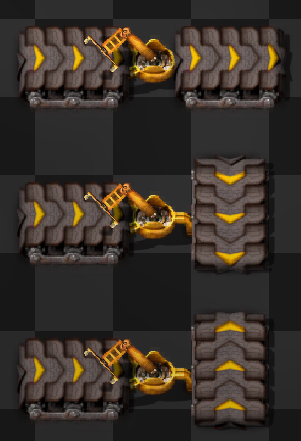
\includegraphics[width=\textwidth]{Figures//captures_joc/redundant_inserter.png}
        \caption{Combinacions redundants cinta-inseridor}
    \end{subfigure}
    \hfill
    \begin{subfigure}{0.45\textwidth}
        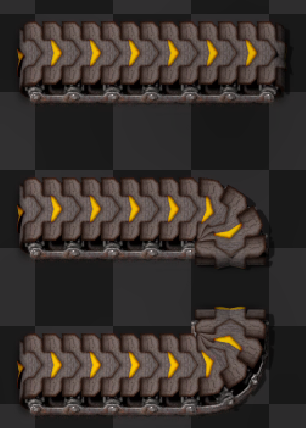
\includegraphics[width=\textwidth]{Figures//captures_joc/conveyor_alternative.png}
        \caption{Alternativa vàlida només amb cintes}
    \end{subfigure}
    \caption{Casos on un inseridor és redundant i pot ser substituït per una cinta obtenint el mateix resultat}
    \label{fig:redundant_inserter}
\end{figure}

Els casos on la cinta no apunta a l'inseridor els hem de permetre, ja que es tracten de bifurcacions a les rutes i són completament vàlides. De la mateixa manera si la cinta apunta a l'inseridor per la sortida d'aquest és un assemblador també l'hem de permetre, ja que una cinta per si sola no pot afegir objectes a un assemblador.\\

La restricció que implementa aquesta millora és força senzilla:

\begin{lstlisting}[language=Python, caption=Evitar inserdiors redundants]
for each cell (i, j) in the grid of size (height x width):
    prevent = []
    for each dir in [north, east, south, west]:
        in_x = i + displacement[dir][0]
        in_y = j + displacement[dir][1]
        out_x = i + displacement[opposite_dir[dir]][0]
        out_y = j + displacement[opposite_dir[dir]][1]
        if 0 <= in_x < height and 0 <= in_y < width and 0 <= out_x < height and 0 <= out_y < width:
        prevent.append(Implies(
                        And(inserter[i][j] == opposite_dir[dir],
                            inserter[i][j] == conveyor[in_x][in_y]),
                        conveyor[out_x][out_y] == empty))
    assert Implies(inserter[i][j] != empty, And(prevent))
\end{lstlisting}

El que es fa és, per cada casella \texttt{i j}, i per cada possible direcció, s'agafen les caselles d'entrada i sortida relatives a la direcció i la posició (\texttt{in\_x, in\_y, out\_x, out\_y}), si el valor de la variable \texttt{inserter[i][j]} és igual a la direcció oposada que estem mirant, és a dir la casella d'entrada, i la casella d'entrada és una cinta amb direcció igual a l'inseridor (cas que volem detectar), llavors a la casella de sortida de l'inseridor no hi pot haver una cinta, sigui quina sigui la seva direcció, d'aquesta mare prevenim les combinacions redundants entre cintes i inseridors.

\begin{figure}[H]
    \centering
    \begin{subfigure}{0.45\textwidth}
        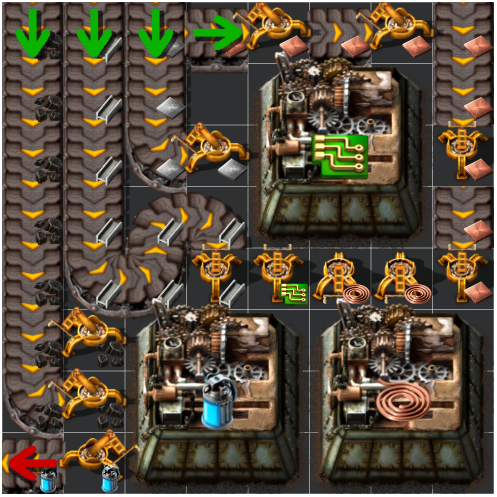
\includegraphics[width=\textwidth]{Figures//captures_joc/exemples_model/instancia_amb_redundancia.PNG}
        \caption{Sense aplicar la restricció}
    \end{subfigure}
    \hfill
    \begin{subfigure}{0.45\textwidth}
        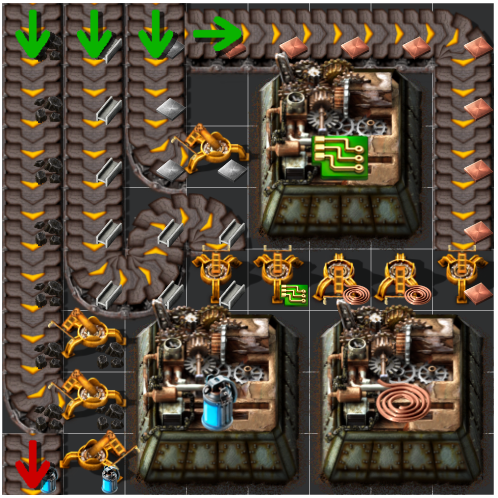
\includegraphics[width=\textwidth]{Figures//captures_joc/exemples_model/instancia_sense_redundancia.PNG}
        \caption{Aplicant la restricció}
    \end{subfigure}
    \caption{Comparació de la mateixa instància sense i aplicant la millora}
\end{figure}

\section{Criteris d'optimització}
Al model s'han incorporat tres criteris d'optimització diferents. N'hi ha un que és el bàsic i sempre es té en compte que és el que maximitza el nombre d'objectes produïts. Aquest criteri se li pot sumar l'optimització addicional que redueix el nombre d'elements que formen part d'una ruta i l'optimització que redueix la pèrdua d'objectes.\\
Tot seguit s'expliquen en detall els criteris d'optimització i les seves implementacions.

\subsection{Maximitzar la quantitat d'objectes}
Per poder maximitzar la quantitat d'objectes que surten del blueprint, cal poder identificar les variables \texttt{item\_flow\_rate} a les posicions de sortida del blueprint. Això ho podem fer de manera molt senzilla, ja que les posicions de sortida del blueprint tracten d'un dels inputs del model. A partir d'aquí, només cal maximitzar la suma d'objectes a les posicions de sortida. Això s'ha fet de la següent manera:
\begin{lstlisting}[language=Python, caption=Quantitat d'objectes de sortida]
    def item_output(self):
        item_output = []
        for pos in output:
            i = pos[0]
            j = pos[1]
            item_output.append(output_flow_rate[i][j])
        return sum(item_output)
\end{lstlisting}

La implementació és molt senzilla, ja que el model es guarda en una llista de llistes \texttt{output} les coordenades al blueprint de cada casella de sortida, així que iterant per aquestes coordenades i fent el sumatori de la variable \texttt{item\_flow\_rate} a les posicions corresponents, només cal dir-li a l'optimitzador de Z3 que maximitzi aquest sumatori:

\begin{lstlisting}[language=Python, caption=Maximitzar el criteri]
    opt = Optimize()
    opt.maximize(item_flow_rate_behaviour.item_output())
\end{lstlisting}

\subsection{Minimitzar la mida de les rutes}
\subsection{Minimitzar la pèrdua d'objectes}






% Indicate the main file. Must go at the beginning of the file.
% !TEX root = ../main.tex

%----------------------------------------------------------------------------------------
% CHAPTER TEMPLATE
%----------------------------------------------------------------------------------------


\chapter{Disseny del front end} % Main chapter title

\label{Disseny del front end} % Change X to a consecutive number; for referencing this chapter elsewhere, use \ref{ChapterX}

%----------------------------------------------------------------------------------------
% SECCIÓ 1: Disseny del front end
%----------------------------------------------------------------------------------------
Aquest treball no se centra en el desenvolupament d'una aplicació o producte i el front end s'ha fet per presentar un treball complet i per facilitar l'anàlisi i generació de les instàncies. Als següents apartats es fa una explicació de com s'ha dissenyat aquesta part del treball sense entrar molt en detall, ja que aquest no és l'enfocament principal del projecte.

\section{Distribució de la pàgina web}
Com s'ha explicat per fer la interfície d'usuari s'ha optat per fer-la en una web. Aquesta està distribuïda en tres parts:
\subsection{Pàgina principal}
La pàgina principal és on es rep l'usuari, aquesta conté una breu descripció del projecte i com usar la web. A més també inclou un menú a la dreta amb el qual es pot navegar als dos apartats principals, la generació d'instàncies i la visualització d'instàncies, la distribuació de la pàgina principal es pot veure a la figura \ref{fig:home-webpage}.\\

\begin{figure}[H]
    \centering
    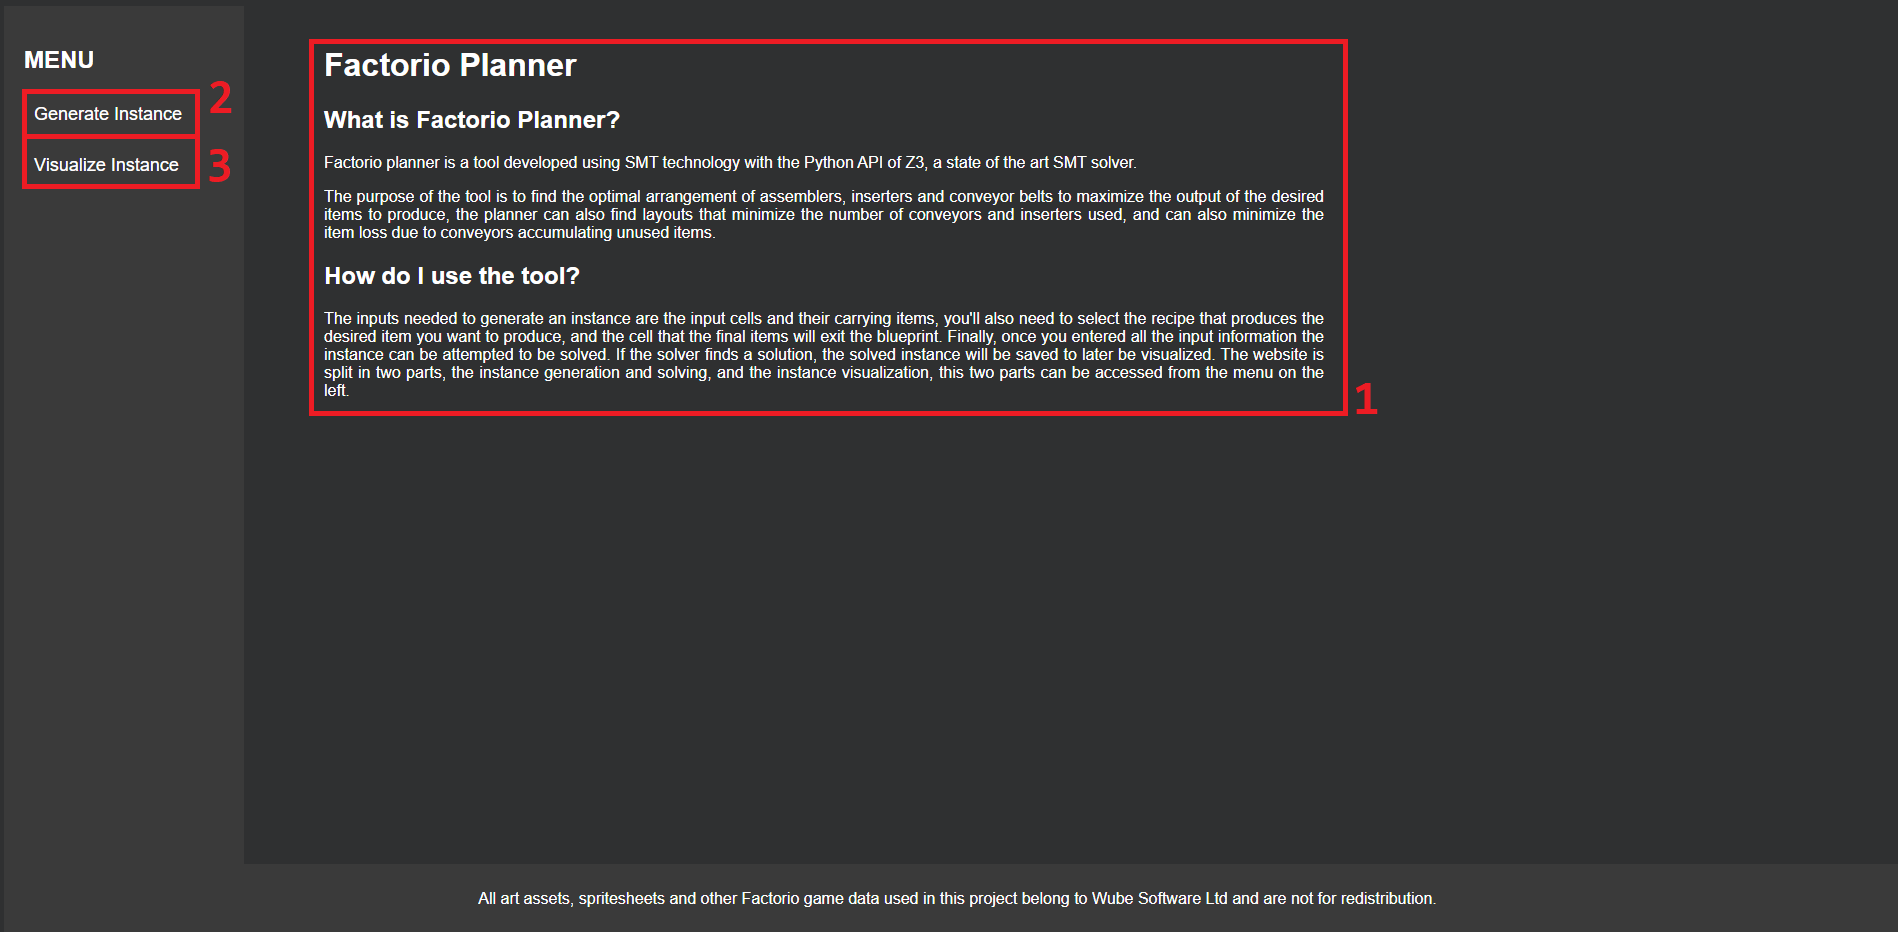
\includegraphics[width=1\linewidth]{Figures//captures_web/home_web.png}
    \caption{Plana principal de la web (1.Descripció de la web, 2.Opció del menú per generar instàncies, 3.Opció del menú per visualitzar instàncies)}
    \label{fig:home-webpage}
\end{figure}

\subsection{Generar instàncies}\label{subsec:generar-instancies}
Una de les funcionalitats principals de la interfície és poder generar instàncies de manera automàtica. Aquesta funcionalitat es troba a l'apartat \textit{Generate Instance} de la pàgina web. Des d'aquí sobre una pàgina nova la qual està separada en 4 seccions. Les tres primeres seccions són per afegir la informació d'entrada pel model:

\subsubsection{Objecte a produir}
En aquest apartat s'ha de seleccionar l'arxiu on es guarden totes les receptes del joc, concretament es troba al directori \lstinline{/recipes} del projecte. Amb l'arxiu carregat es pot seleccionar l'objecte que es vol produir i a la web es carrega quins objectes es necessiten per fabricar-lo i en cas que l'objecte depengui de més receptes aquestes es mostraran juntament amb els objectes addicionals requerits per produir-los. D'aquesta manera és molt còmode saber els objectes i receptes implicats.
\begin{figure}[H]
    \centering
    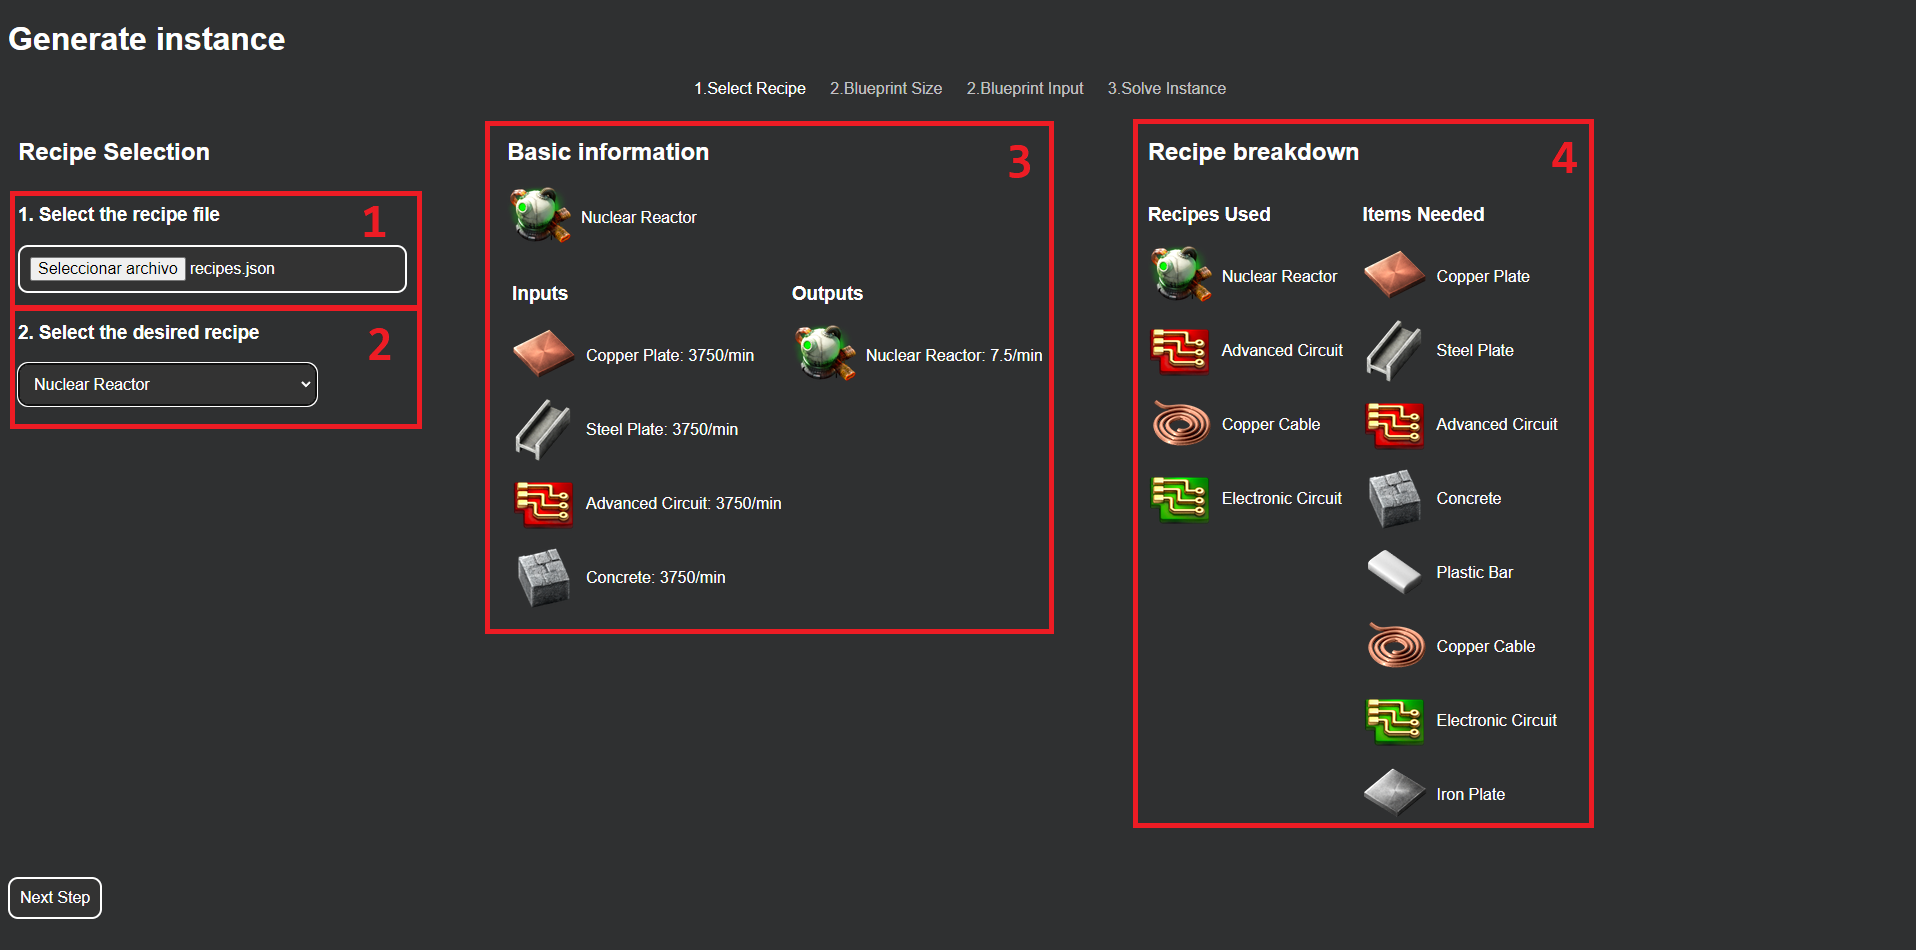
\includegraphics[width=1\linewidth]{Figures//captures_web/generate_instance_recipe_web.png}
    \caption{Primera part de la generació d'una instància (1.Seleccionar arxiu amb les receptes, 2.Seleccionar objecte a produir, 3.Informació de la recepta que produeix l'objecte), 4.Receptes implicades en la producció de l'objecte els objectes implicats)}
    \label{fig:generate_instance_recipe}
\end{figure}

\subsubsection{Mida del blueprint}
Aquest apartat és molt simple, només tracta de dos inputs d'HTML on s'han d'entrar les dimensions del blueprint.
\begin{figure}[H]
    \centering
    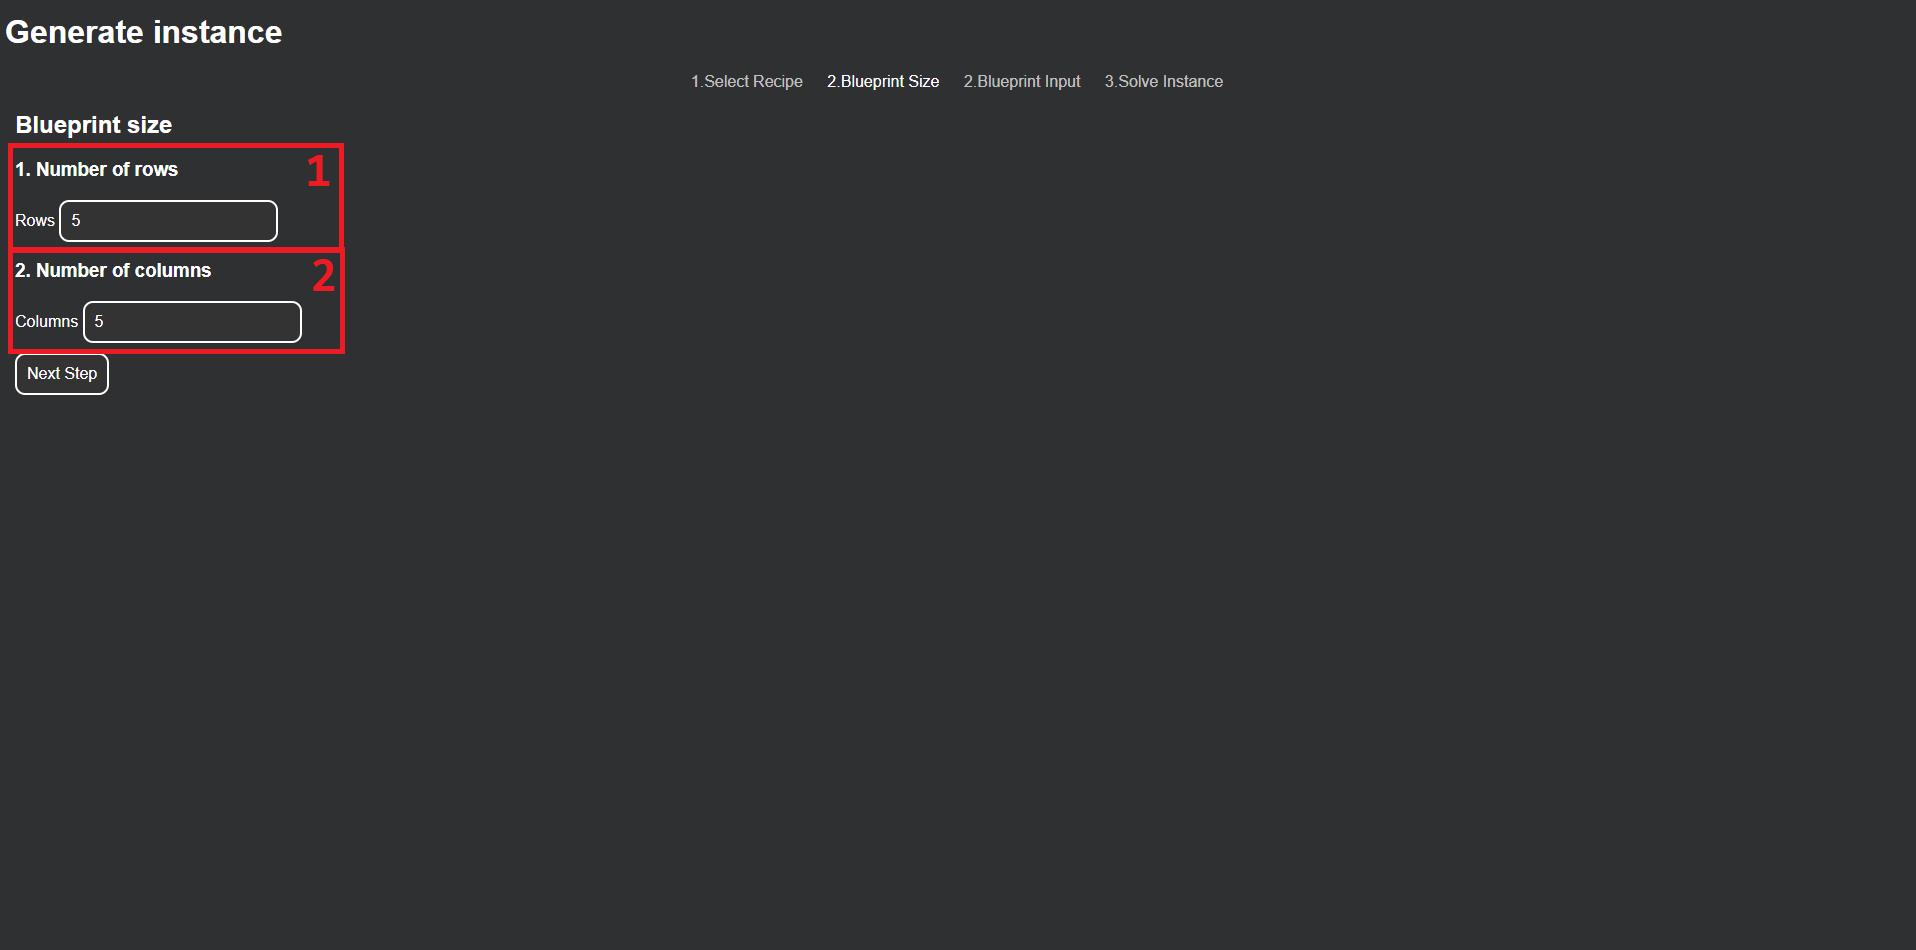
\includegraphics[width=1\linewidth]{Figures//captures_web/generate_instance_size_web.png}
    \caption{Plana web amb el pas 2 on s'ha de seleccionar la mida del blueprint (1.Seleccionar el nombre de files, 2.Seleccionar el nombre de columnes)}
    \label{fig:generate_instance_size}
\end{figure}

\subsubsection{Entrades i sortides del blueprint}
La selecció de quines caselles són d'entrada i sortida i el tipus objectes que han de transportar, és una de les parts més importants de les entrades del model i també una de les més complexes d'implementar, ja que implica poder clicar en una graella, seleccionar l'objecte i determinar si és una casella d'entrada i sortida, tot això mantenint una retroacció visual per saber el que s'està fent.\\

El funcionament és el següent, en funció de la mida entrada a la secció anterior i la recepta seleccionada al primer apartat del generador d'instàncies, aquesta part conté una graella interactiva on podem fer clic esquerre sobre les caselles i a la dreta de la graella apareixerà la informació relativa a la casella. Aquesta informació ens diu quin objecte conté el qual es pot seleccionar en un desplegable que contindrà els objectes que es necessiten per produir l'objecte objectiu, a més també ens diu si la casella és d'entrada o sortida.\\
Quan se seleccioni un objecte aquest es mostra a la graella de forma visual juntament amb un punt verd que indica que la casella és d'entrada. En cas que se seleccioni com a casella de sortida, es mostra un punt vermell.

\begin{figure}[H]
    \centering
    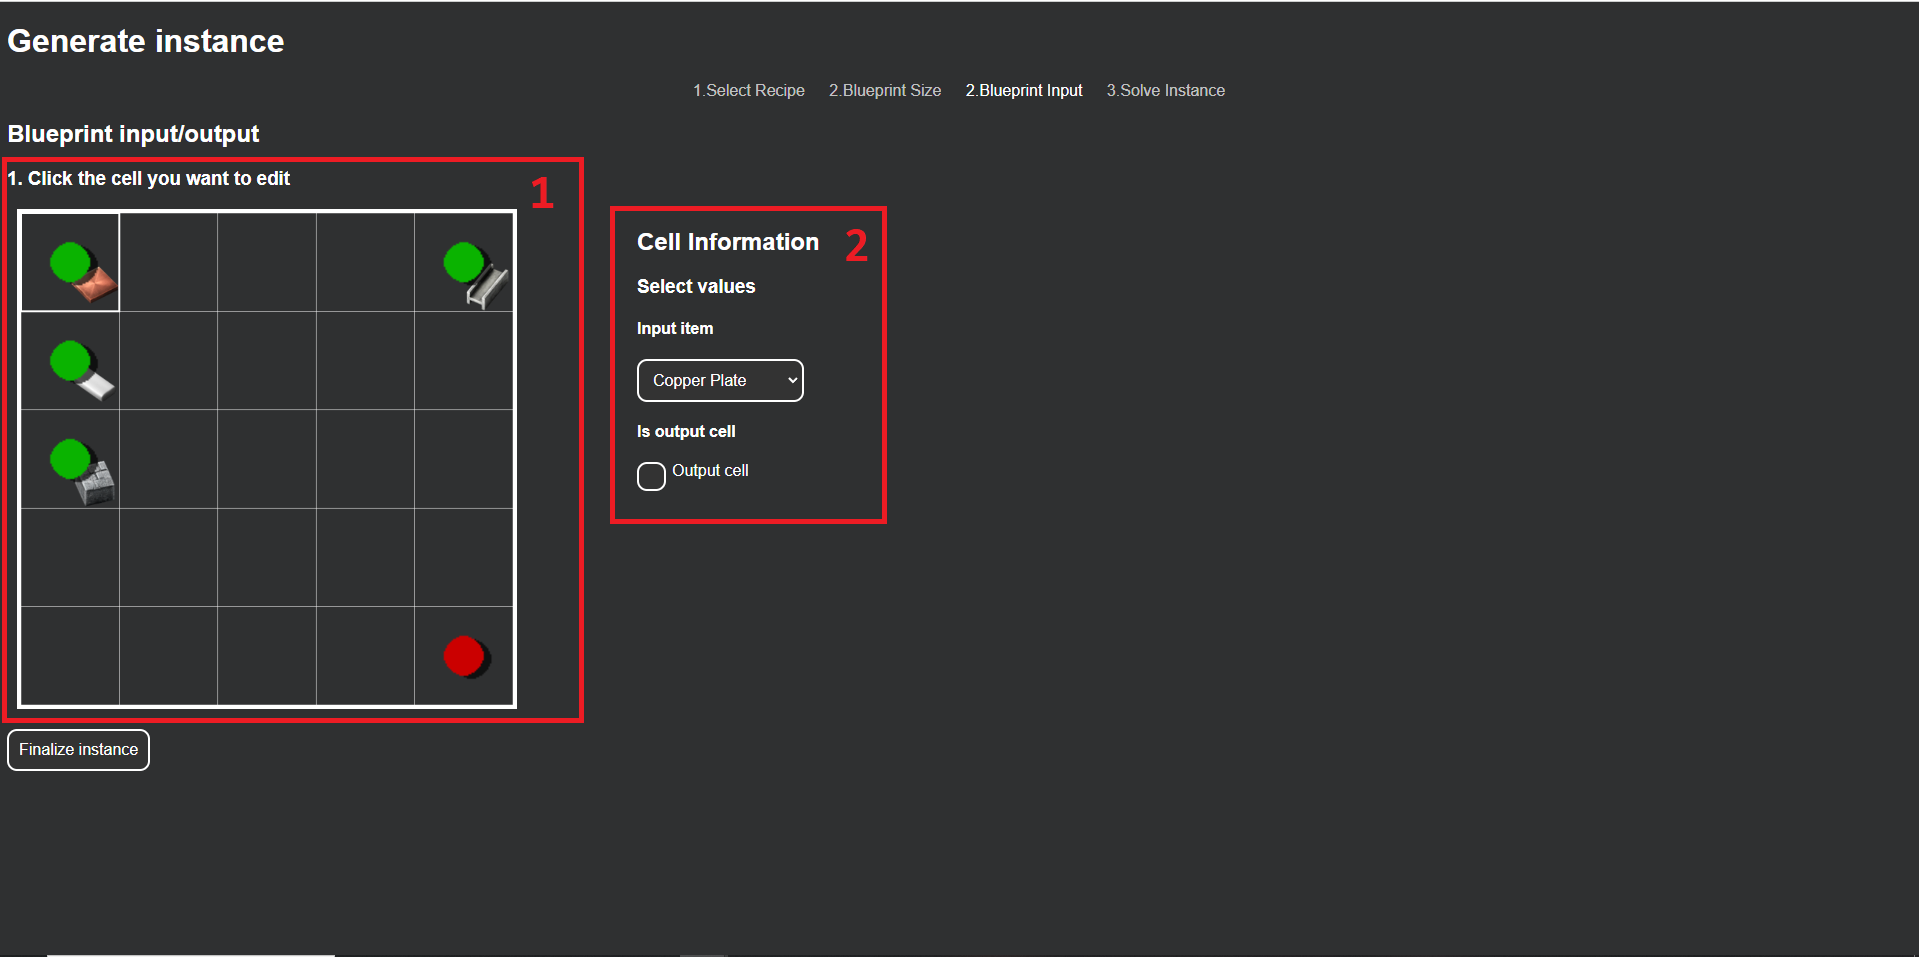
\includegraphics[width=1\linewidth]{Figures//captures_web/generate_instance_input_web.png}
    \caption{Plana web amb el pas 3 on s'han de seleccionar les entrades i sortides del blueprint (1.Graella interactiva, 2.Informació de la casella seleccionada)}
    \label{fig:generate_instance_input}
\end{figure}

\subsubsection{Resoldre la instància}
L'últim pas del procés de la generació de la instància tracta de seleccionar el criteri d'optimització i enviar la instància al back-end perquè sigui solucionada. Si la instància és resolta, s'informa el temps que tarda i l'estat (SAT, UNSAT o TIMED OUT), tot seguit es pot clicar el botó de descarregar la instància resolta per ser visualitzada a l'apartat de la web del visualitzador d'instàncies.
\begin{figure}[H]
    \centering
    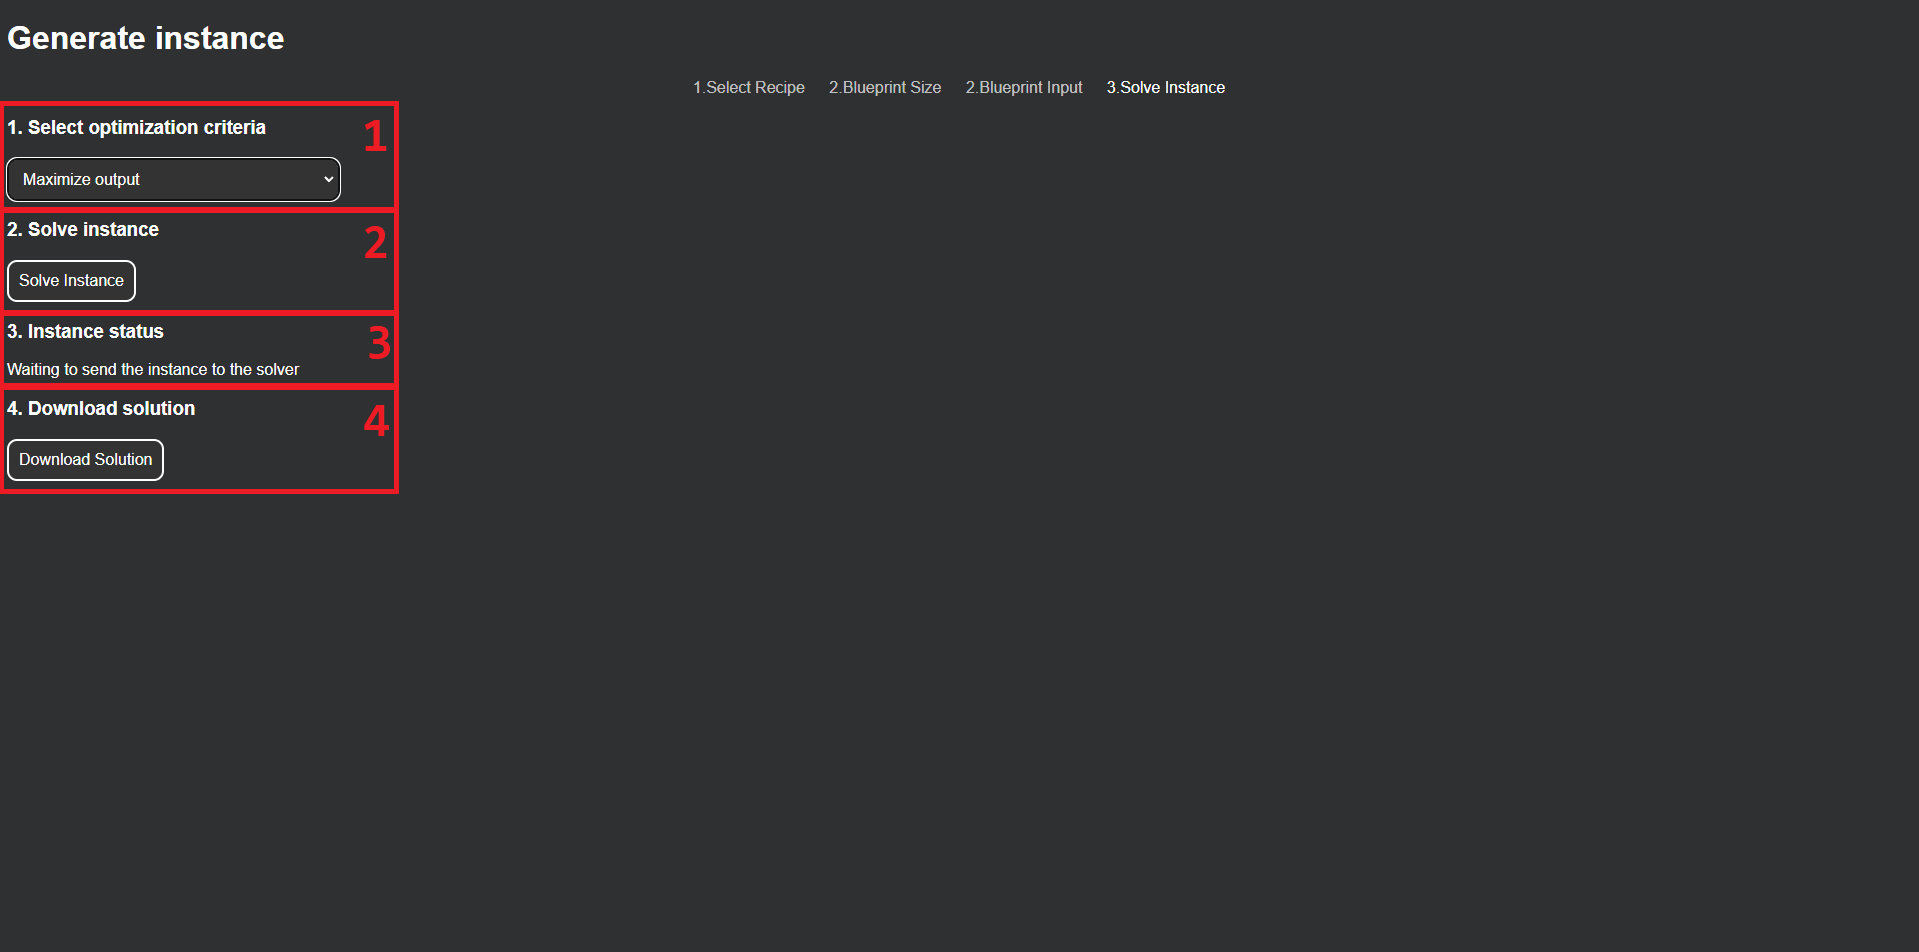
\includegraphics[width=1\linewidth]{Figures//captures_web/generate_instance_solving_web.PNG}
    \caption{Últim pas de la generació de la instància (1.Seleccionar l'objectiu d'optimització, 2.Botó per enviar la instància a resoldre, 3.Informació amb l'estat del procés de solving, 4.Botó per baixar el fitxer amb la solució a la instància)}
    \label{fig:generate_instance_solving}
\end{figure}


\subsection{Visualitzar instàncies}
La segona part del front end tracta del visualitzador d'instàncies, aquest té la seva pròpia pàgina HTML, que es pot veure a la figura \ref{fig:visualize_basic}. La interacció, de manera similar a la selecció d'entrades i sortides del generador d'instàncies, es fa mitjançant un canvas el qual conté tota la part interactiva i s'encarrega de mostrar de manera visual tota la informació relativa a cada casella de la instància resolta.\\
A més també hi ha una part a l'HTML que mostra informació més detallada de la casella, el tipus d'objectes que transporta, quantitats... En cas que la casella seleccionada tracti d'un assemblador es mostra informació addicional com la recepta que produeix les quantitats d'entrada i sortida i les seves ràtios. A la figura \ref{fig:solved_instance_web} es pot veure com queda representada la informació d'una instància a la web, on les fletxes verdes indiquen les caselles d'entrada de materials i les fletxes vermelles les caselles de sortida del \textit{blueprint}.\\
A la figura \ref{fig:error_caprure_web}, es pot veure com la web detecta possibles errors amb la instància que es vol obrir ja sigui perquè no s'ha pogut resoldre (TIMED OUT, UN-SAT) o bé perquè per alguna raó l'arxiu JSON no conté tots els camps que s'esperen o directament no és el format esperat.

\begin{figure}[H]
    \centering
    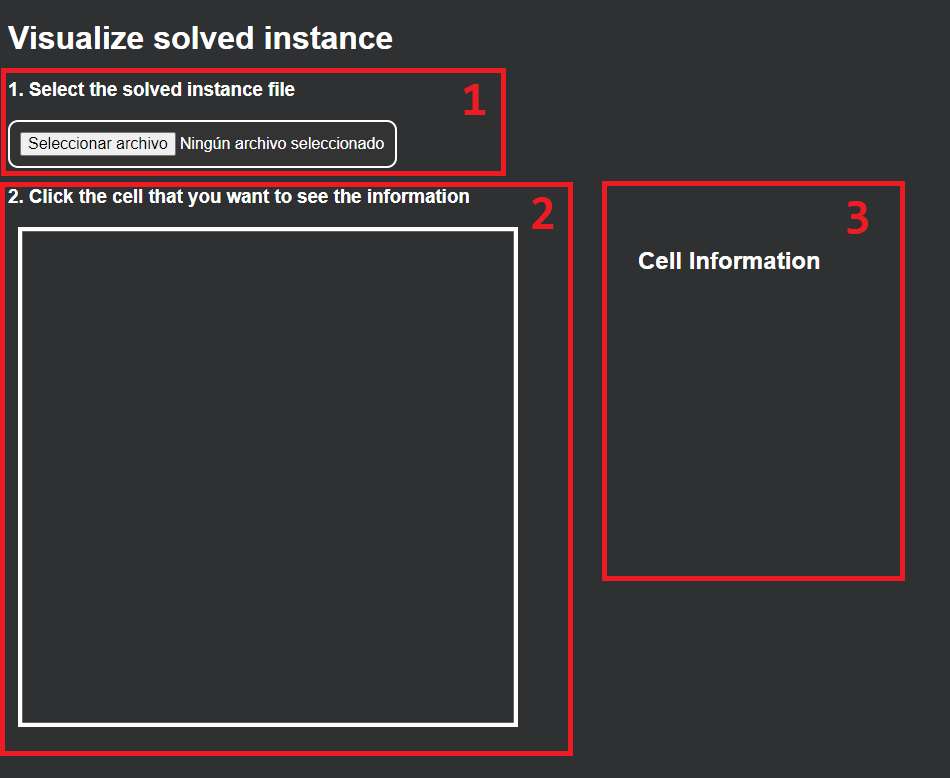
\includegraphics[width=1\linewidth]{Figures//captures_web/visualize_instance_basic.PNG}
    \caption{Distribució dels elements (1.Seleccionador d'instàncies resoltes, 2.Canvas on es mostra la informació de la instància, 3.Informació especifica de la casella seleccionada)}
    \label{fig:visualize_basic}
\end{figure}


\begin{figure}[H]
    \centering
    \begin{subfigure}{0.45\textwidth}
        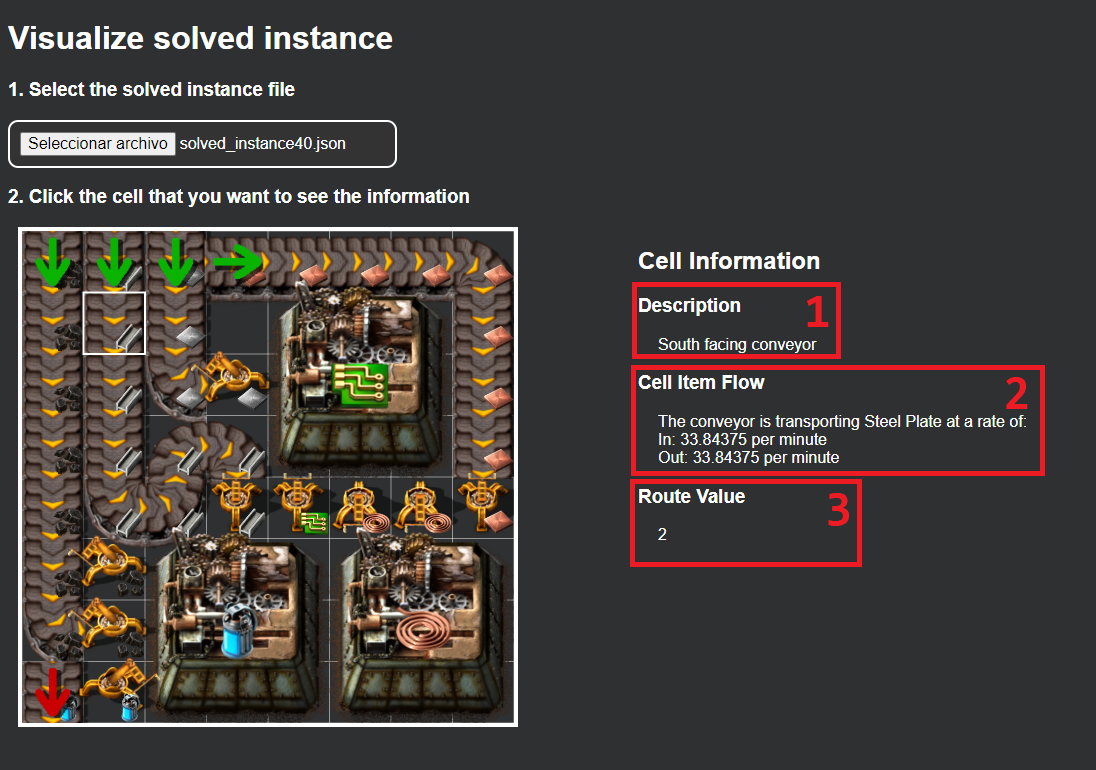
\includegraphics[width=\textwidth]{Figures/captures_web/visualize_instance_sat_conv.png}
        \caption{Informació d'una cinta (1.Breu descripció de la casella, 2.Quantitat d'objectes que entren i surten de la cinta, 3.Valor de ruta que té la cinta)}
    \end{subfigure}
    \hfill
    \begin{subfigure}{0.45\textwidth}
        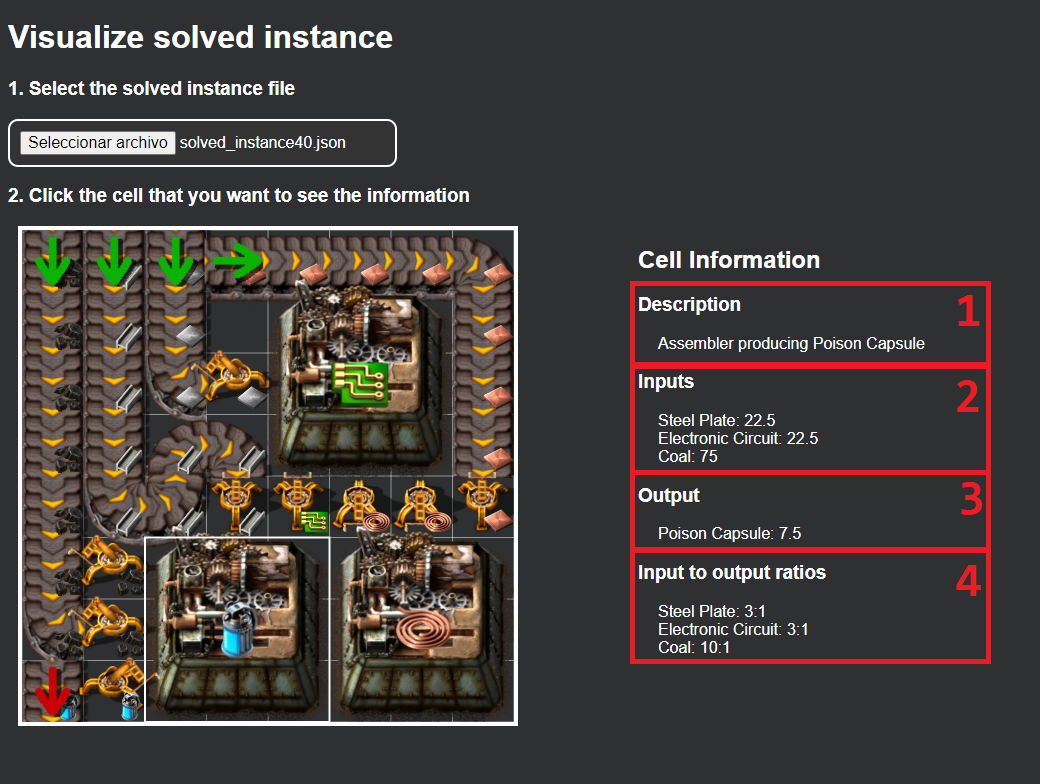
\includegraphics[width=\textwidth]{Figures/captures_web/visualize_instance_sat_ass.png}
        \caption{Informació d'un assemblador (1.Breu descripció de la casella, 2.Objectes i quantitats que entren a l'assemblador, 3.Objecte i quantitat que l'assemblador produeix, 4.Ràtios entre els objectes d'entrada i l'objecte produït)}
    \end{subfigure}
    \caption{Exemple de com es veu una instància resolta i la informació dels seus elements}
    \label{fig:solved_instance_web}
\end{figure}

\begin{figure}[H]
    \centering
    \begin{subfigure}{0.3\textwidth}
        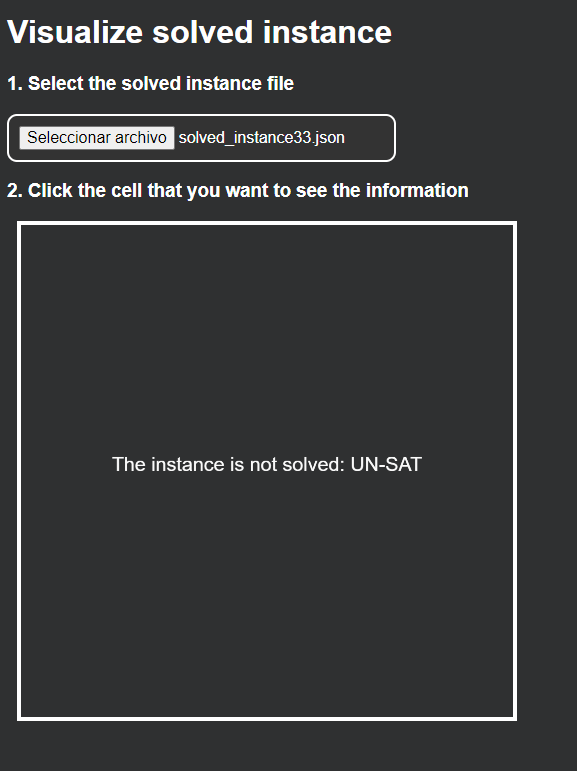
\includegraphics[width=\textwidth]{Figures/captures_web/visualize_instance_unsat.PNG}
        \caption{Instància sense solució}
    \end{subfigure}
    \hfill
    \begin{subfigure}{0.3\textwidth}
        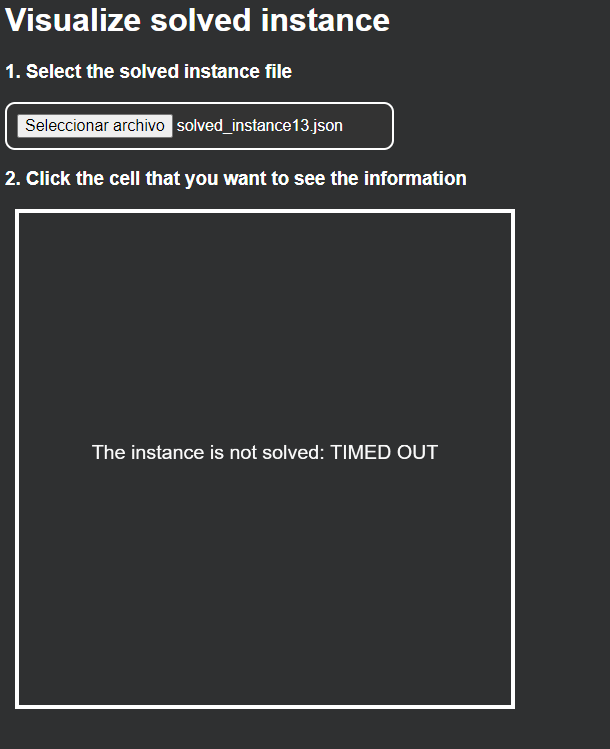
\includegraphics[width=\textwidth]{Figures/captures_web/visualize_instance_time_out.PNG}
        \caption{Instància no resolta}
    \end{subfigure}
    \hfill
    \begin{subfigure}{0.3\textwidth}
        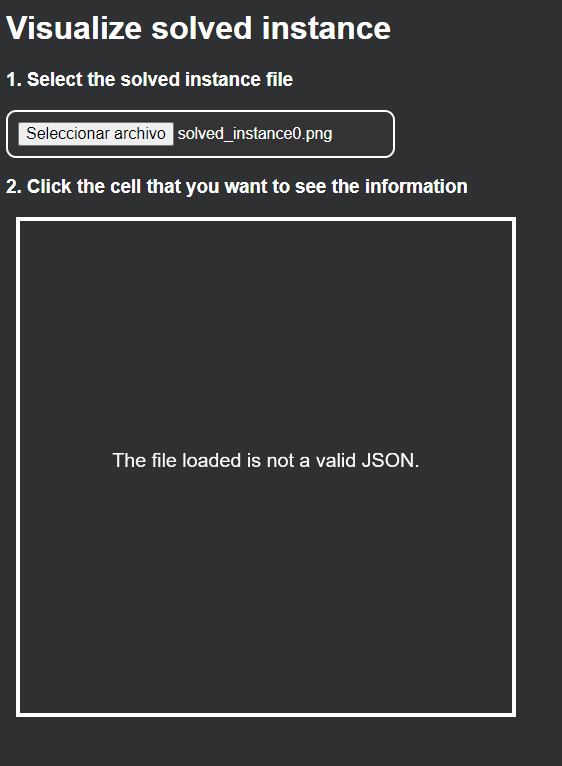
\includegraphics[width=\textwidth]{Figures/captures_web/visualize_instance_incorrect_file.PNG}
        \caption{Fitxer incorrecte}
    \end{subfigure}
    \caption{Exemples de com es capturen i mostren diferents errors}
    \label{fig:error_caprure_web}
\end{figure}


\section{Implementació de la pàgina web}
Com s'ha pogut veure a l'apartat anterior la pàgina es divideix en dos apartats principals, la generació i la visualització de les instàncies. Les dues parts, tot i complir funcionalitats diferents, comparteixen molts aspectes sobretot pel que fa a la part interactiva del canvas. Per això s'ha decidit usar el mecanisme d'herència de JavaScript per poder implementar funcionalitats comunes entre les dues parts i després implementar funcionalitats específiques per separat. A continuació l'explicació en detall de com s'ha fet el disseny de la part interactiva amb canvas i ús d'herència.

\subsection{Disseny del canvas interactiu}
El canvas és un element bàsic d'HTML que permet dibuixar imatges, formes geomètriques, text... Per aquest projecte s'ha decidit usar pel fet que no depèn d'altres llibreries i no afegeix més capes de complexitat al projecte.\\
Aquest element s'ha usat en dues parts de la web, a la generació d'instàncies, concretament a l'hora de seleccionar per quines caselles entren els materials i quines caselles són de sortida i per mostrar tots els elements de les instàncies resoltes.\\

Com hi ha moltes funcionalitats que són iguals tant al canvas de generació d'instàncies com el de visualització, s'ha optat per crear una classe abstracta \lstinline{Blueprint}, que conté els atributs compartits com mida, casella seleccionada, la referència a l'element canvas HTML, nombre de files, nombre de columnes, informació de la graella... A més també implementa els mètodes encarregats de dibuixar la graella, detectar els clics a les caselles, actualitzar la informació d'una casella seleccionada... Finalment també obliga a les classes que hereten d'ella a implementar el mètode encarregat de reiniciar el canvas. El diagrama de classes del \lstinline{Blueprint} es pot veure a la figura \ref{fig:blueprint_class_diagram}.

\begin{figure}[H]
    \centering
    \resizebox{\textwidth}{!}{
        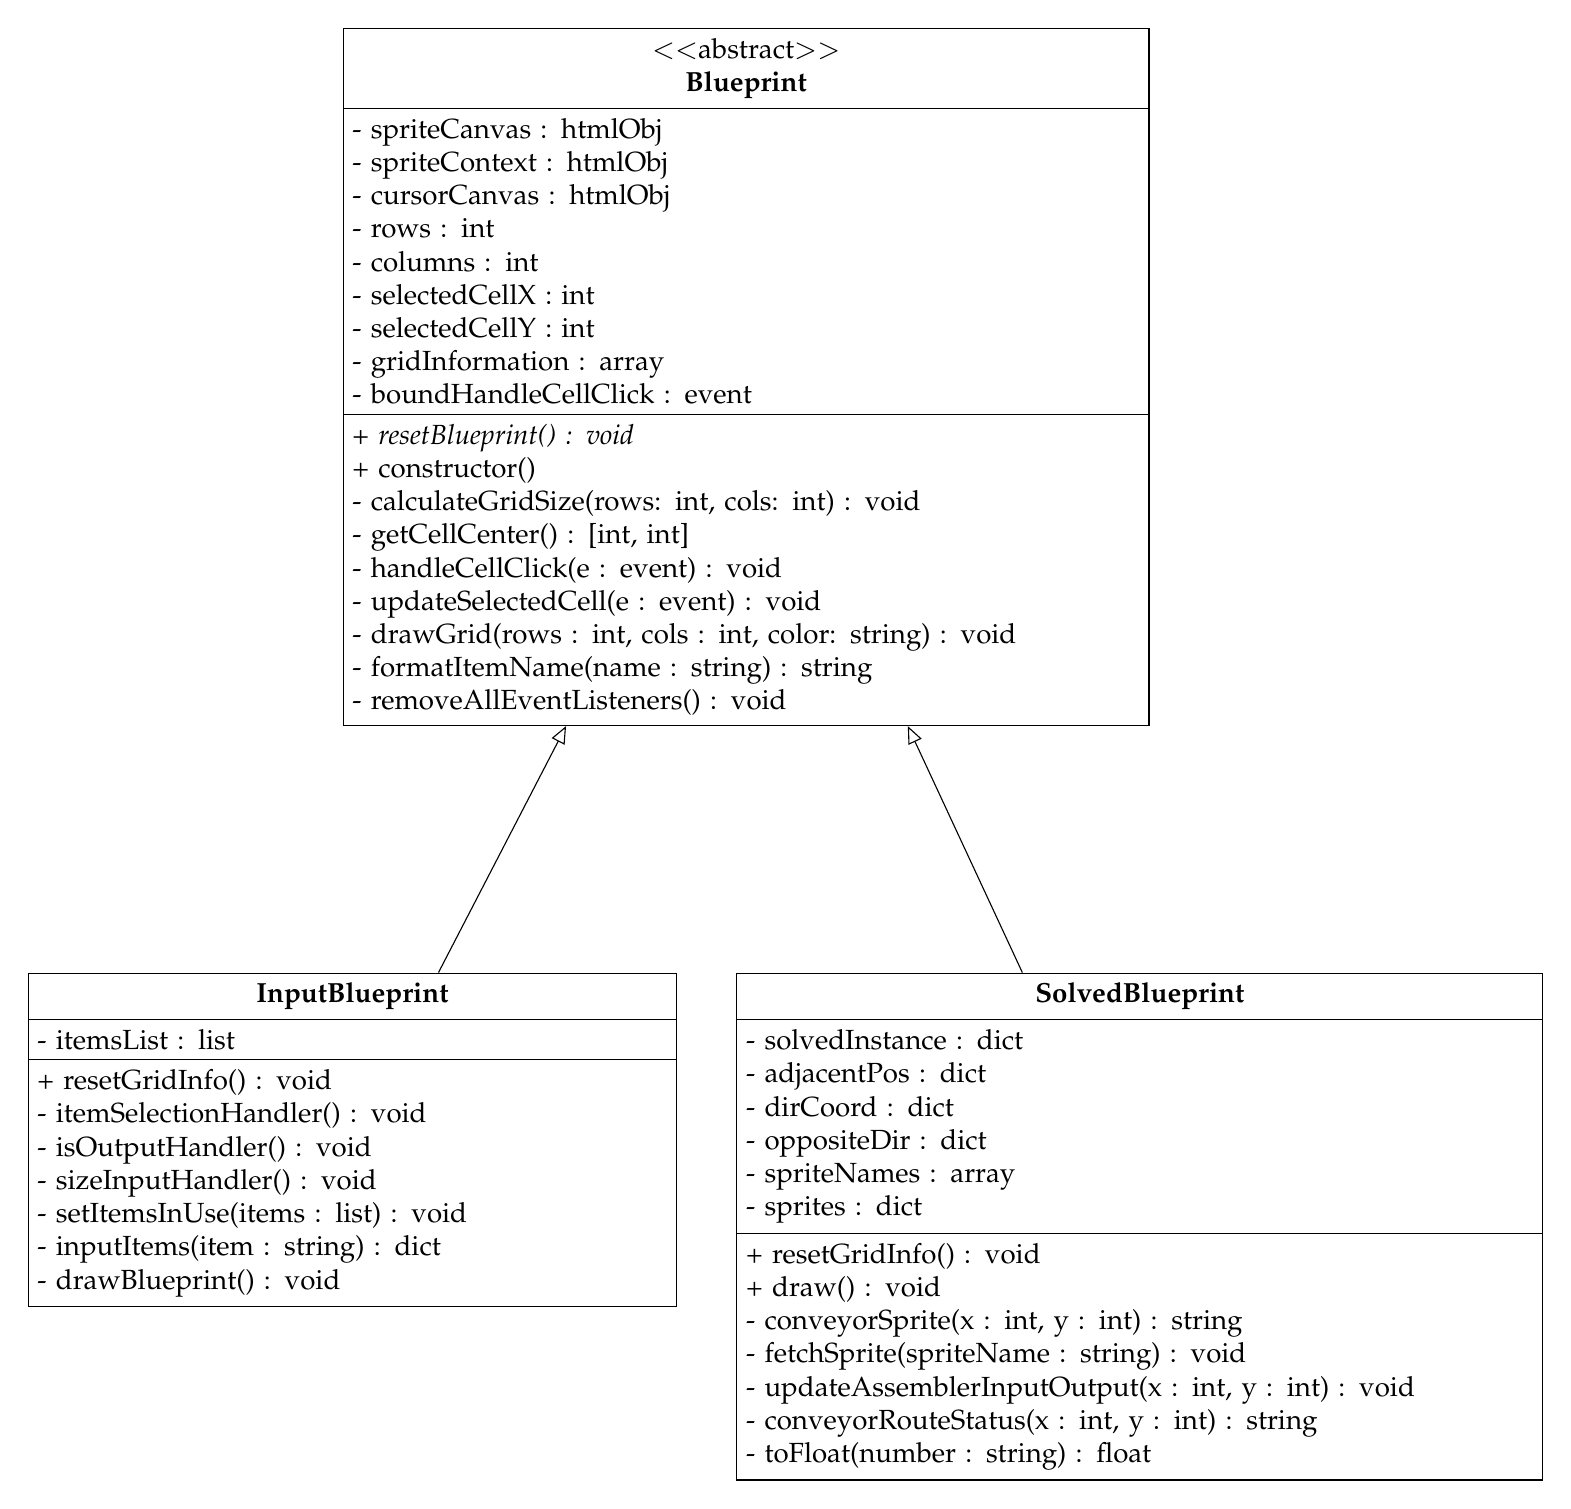
\begin{tikzpicture}
            \begin{abstractclass}[text width=10cm]{Blueprint}{0,0}
                \attribute{- spriteCanvas : htmlObj}
                \attribute{- spriteContext : htmlObj}
                \attribute{- cursorCanvas : htmlObj}
                \attribute{- rows : int}
                \attribute{- columns : int}
                \attribute{- selectedCellX : int}
                \attribute{- selectedCellY : int}
                \attribute{- gridInformation : array}
                \attribute{- boundHandleCellClick : event}
                \operation[0]{+ resetBlueprint() : void}
                \operation{+ constructor()}
                \operation{- calculateGridSize(rows: int, cols: int) : void}
                \operation{- getCellCenter() : [int, int]}
                \operation{- handleCellClick(e : event) : void}
                \operation{- updateSelectedCell(e : event) : void}
                \operation{- drawGrid(rows : int, cols : int, color: string) : void}
                \operation{- formatItemName(name : string) : string}
                \operation{- removeAllEventListeners() : void}
            \end{abstractclass}
            
            \begin{class}[text width=8cm]{InputBlueprint}{-5, -12}
                \inherit{Blueprint}
                \attribute{- itemsList : list}
                \operation{+ resetGridInfo() : void}
                \operation{- itemSelectionHandler() : void}
                \operation{- isOutputHandler() : void}
                \operation{- sizeInputHandler() : void}
                \operation{- setItemsInUse(items : list) : void}
                \operation{- inputItems(item : string) : dict}
                \operation{- drawBlueprint() : void}
            \end{class}
            
            \begin{class}[text width=10cm]{SolvedBlueprint}{5, -12}
                \inherit{Blueprint}
                \attribute{- solvedInstance : dict}
                \attribute{- adjacentPos : dict}
                \attribute{- dirCoord : dict}
                \attribute{- oppositeDir : dict}
                \attribute{- spriteNames : array}
                \attribute{- sprites : dict}
                \operation{+ resetGridInfo() : void}
                \operation{+ draw() : void}
                \operation{- conveyorSprite(x : int, y : int) : string}
                \operation{- fetchSprite(spriteName : string) : void}
                \operation{- updateAssemblerInputOutput(x : int, y : int) : void}
                \operation{- conveyorRouteStatus(x : int, y : int) : string}
                \operation{- toFloat(number : string) : float}
            \end{class}
        \end{tikzpicture}
    }
    \caption{Diagrama de classes amb l'estructura seguida per implementar els canvas interactius}
    \label{fig:blueprint_class_diagram}
\end{figure}


Una part molt important del canvas interactiu és com emmagatzemar la informació de cada casella. Com hi ha diferents tipus de casella i cadascuna ha de guardar informació diferent i s'ha de representar gràficament al canvas de manera diferent, s'ha decidit guardar de la següent manera:

\subsubsection{Estructura de dades per guardar la informació de la graella}
Per guardar la informació de cada casella s'ha fet de manera similar a la classe \lstinline{Blueprint}. S'ha creat una classe abstracta \lstinline{Cell} que conté la informació que totes les caselles comparteixen i després s'han creat diferents classes que hereten d'aquesta i implementen els seus mètodes específics, d'aquesta manera es pot tenir una matriu, en aquest cas \lstinline{gridInformation}, amb cel·les que parteixen de la mateixa classe pare i implementen el mateix mètode de maneres diferents, permetent així tenir un codi més net i genèric.\\
L'estructura de classes, atributs i mètodes es pot veure a la figura \ref{fig:cell_class_diagram}.


\begin{figure}[H]
    \centering
    \rotatebox{90}{
        \scalebox{0.65}{
            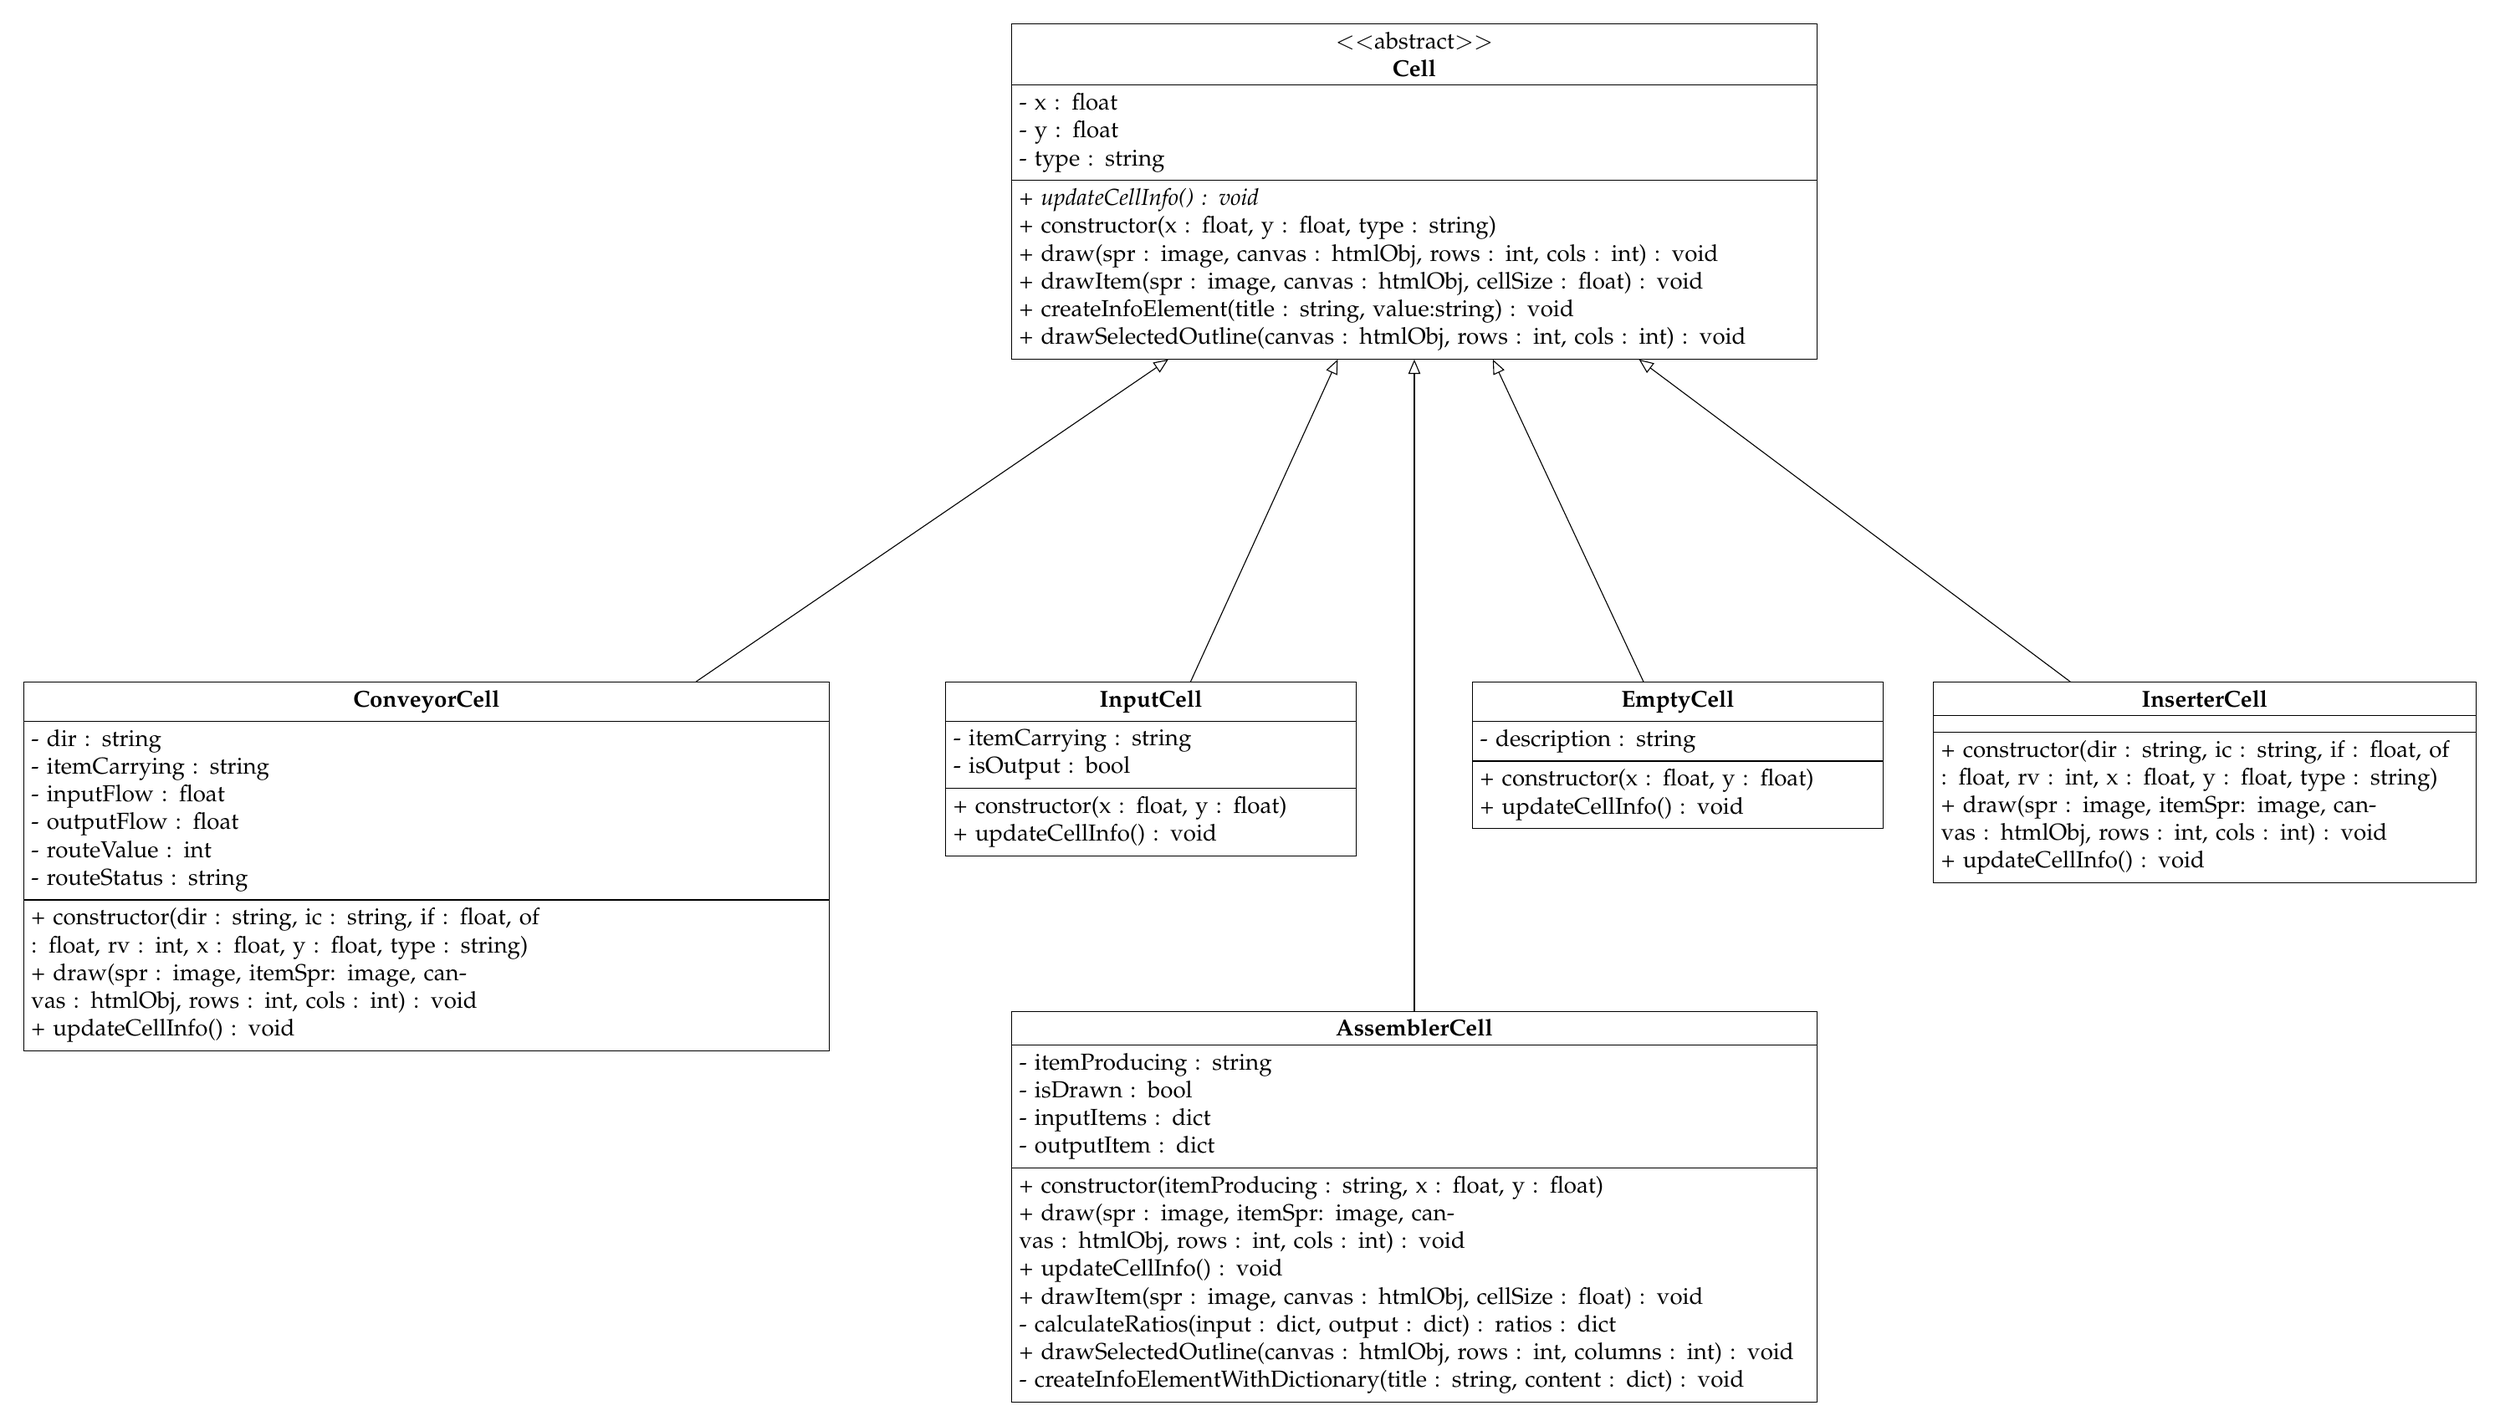
\begin{tikzpicture}
                \begin{abstractclass}[text width=12cm]{Cell}{0,0}
                    \attribute{- x : float}
                    \attribute{- y : float}
                    \attribute{- type : string}
                    \operation[0]{+ updateCellInfo() : void}
                    \operation{+ constructor(x : float, y : float, type : string)}
                    \operation{+ draw(spr : image, canvas : htmlObj, rows : int, cols : int) : void}
                    \operation{+ drawItem(spr : image, canvas : htmlObj, cellSize : float) : void}
                    \operation{+ createInfoElement(title : string, value:string) : void}
                    \operation{+ drawSelectedOutline(canvas : htmlObj, rows : int, cols : int) : void}

                \end{abstractclass}
                
                \begin{class}[text width=12cm]{ConveyorCell}{-15, -10}
                    \inherit{Cell}
                    \attribute{- dir : string}
                    \attribute{- itemCarrying : string}
                    \attribute{- inputFlow : float}
                    \attribute{- outputFlow : float}
                    \attribute{- routeValue : int}
                    \attribute{- routeStatus : string}
                    \operation{+ constructor(dir : string, ic : string, if : float, of : float, rv : int, x : float, y : float, type : string)}
                    \operation{+ draw(spr : image, itemSpr: image, canvas : htmlObj, rows : int, cols : int) : void}
                    \operation{+ updateCellInfo() : void}
                \end{class}
                
                \begin{class}[text width=8cm]{InserterCell}{12, -10}
                    \inherit{Cell}
                    \operation{+ constructor(dir : string, ic : string, if : float, of : float, rv : int, x : float, y : float, type : string)}
                    \operation{+ draw(spr : image, itemSpr: image, canvas : htmlObj, rows : int, cols : int) : void}
                    \operation{+ updateCellInfo() : void}
                \end{class}

                \begin{class}[text width=12cm]{AssemblerCell}{0, -15}
                    \inherit{Cell}
                    \attribute{- itemProducing : string}
                    \attribute{- isDrawn : bool}
                    \attribute{- inputItems : dict}
                    \attribute{- outputItem : dict}
                    \operation{+ constructor(itemProducing : string, x : float, y : float)}
                    \operation{+ draw(spr : image, itemSpr: image, canvas : htmlObj, rows : int, cols : int) : void}
                    \operation{+ updateCellInfo() : void}
                    \operation{+ drawItem(spr : image, canvas : htmlObj, cellSize : float) : void}
                    \operation{- calculateRatios(input : dict, output : dict) : ratios : dict}
                    \operation{+ drawSelectedOutline(canvas : htmlObj, rows : int, columns : int) : void}
                    \operation{- createInfoElementWithDictionary(title : string, content : dict) : void}
                \end{class}

                \begin{class}[text width=6cm]{InputCell}{-4, -10}
                    \inherit{Cell}
                    \attribute{- itemCarrying : string}
                    \attribute{- isOutput : bool}
                    \operation{+ constructor(x : float, y : float)}
                    \operation{+ updateCellInfo() : void}
                \end{class}

                \begin{class}[text width=6cm]{EmptyCell}{4, -10}
                    \inherit{Cell}
                    \attribute{- description : string}
                    \operation{+ constructor(x : float, y : float)}
                    \operation{+ updateCellInfo() : void}
                \end{class}
            \end{tikzpicture}
        }
    }
    \caption{Diagrama de classes amb l'estructura de les diferents caselles}
    \label{fig:cell_class_diagram}
\end{figure}


Amb aquesta estructura cada casella s'encarrega de com ha de mostrar la seva informació a la web, com dibuixar-se correctament al canvas i com emmarcar-se per fer veure que ha sigut seleccionada.

\subsection{Alguns detalls interessants}
Al llarg de la implementació s'han hagut de prendre algunes decisions que són importants i s'han de mencionar.

\subsubsection{Demanar imatges al servidor}
Els canvas d'HTML dibuixen les imatges en ordre de crida de la funció \lstinline{drawImage}, així que per obtenir el resultat correcte és molt important fer les crides de dibuixat en ordre, això pot semblar una ximpleria si el codi que s'està fent és concurrent, però en cas de les aplicacions web obtenir imatges es fa en paral·lel, ja que s'han de sol·licitar al servidor, fent que si no s'han carregat totes les imatges prèviament, aquestes es dibuixaran en ordre d'arribada fent que l'ordre de dibuixar inicial es perdi. Per arreglar aquest problema s'ha creat una funció que demana al servidor totes les imatges que la instància resolta necessita i aquestes es guarden en un diccionari que més tard es podrà consultar de manera completament síncrona.\\

\begin{lstlisting}[language=Java, caption=Fetch sprite]
    fetchSprite(spriteName){
        return new Promise((resolve, reject) => {
            let img = new Image();
            img.onload = () => resolve(img);
            img.onerror = reject;
            img.src = `/static/${spriteName}.png`;
        });
    }
\end{lstlisting}

Aquesta funció retorna una \lstinline{Promise} d'aquesta manera des de fora, es pot fer un codi que fins que totes les \lstinline{Promise} corresponents a cada imatge no s'hagin resolt, no s'executi cert codi, per exemple es pot fer el següent:

\begin{lstlisting}[language=Java, caption=Fetch all sprites]
    Promise.all(this.spriteNames.map(this.fetchSprite)).then(sprites => {
        this.sprites = Object.fromEntries(this.spriteNames.map((name, i) => [name, sprites[i]]));
           //Codi que s'executara despres de rebre totes les imatges
    });
\end{lstlisting}

Amb aquest tall de codi el que s'està fent és cridar la funció anterior per cada imatge guardada a la llista \lstinline{spriteNames} i fins que no s'han rebut totes no es continua, assegurant així que si després es volen dibuixar les imatges aquestes no s'hagin d'anar a buscar.

\subsubsection{Evitar fer crides de dibuixat innecessàries}
Un altre detall és que si es vol modificar alguna part del que s'hagi dibuixat al canvas HTML, cal esborrar tot el que hi havia, modificar la part desitjada i tornar a dibuixar, això com es pot comprendre només és factible si hi ha moltes parts del canvas que s'estan canviant, però si només és un element no val la pena. Per això s'ha decidit que per emmarcar la casella seleccionada no es faci al mateix canvas on es dibuixen tots els elements sinó que millor crear un segon canvas, superposar-lo al canvas on es dibuixen tots els elements i així només s'ha d'esborrar i redibuixar el quadrat que emmarca les caselles. D'aquesta manera es redueix molt temps de dibuixat quan la majoria d'elements del canvas són estàtcs.\\

Per aconseguir l'efecte de superposició dels canvas s'ha fet el següent:

\begin{lstlisting}[language=html, caption=Declaració dels canvas]
    <div id="canvas-container">
        <canvas id="model-view" width="1000" height="1000">
            Your browser does not support the HTML canvas tag.
        </canvas>
        <canvas id="cursor-canvas" width="1000" height="1000">
            Your browser does not support the HTML canvas tag.
        </canvas>
    </div>
\end{lstlisting}

\begin{lstlisting}[language=html, caption=Estil dels canvas]
    #canvas-container > canvas {
        position:absolute;
        left:0;
        top:0;
    }
\end{lstlisting}

Amb aquesta declaració només cal administrar el comportament de cada canvas des de JavaScript per obtenir el comportament desitjat.








% Indicate the main file. Must go at the beginning of the file.
% !TEX root = ../main.tex

%----------------------------------------------------------------------------------------
% CHAPTER TEMPLATE
%----------------------------------------------------------------------------------------


\chapter{Experimentació} % Main chapter title

\label{Experimentació} % Change X to a consecutive number; for referencing this chapter elsewhere, use \ref{ChapterX}
En aquest apartat s'expliquen en detall els criteris seguits per generar les instàncies, com aquests afecten la seva complexitat i temps de resolució, com s'han obtingut i recollit tots els resultats. També es fa una comparativa del rendiment de cada millora que ha rebut el model.

\section{Generació d'instàncies}
La generació d'instàncies s'ha fet mitjançat la pàgina web desenvolupada \ref{subsec:generar-instancies}, la qual ha ajudat molt a poder captar visualment les implicacions dels inputs del model a la complexitat de les instàncies.\\
A banda un cop generades i guardades les instàncies en fitxer .json, s'ha fet ús d'un script en Python, veure annex \ref{AppendixB}, que itera per tots els fitxers i guarda les dades més importants en un fitxer excel per més tard poder analitzar de forma més fàcil les característiques de cada instància.
Tot i que la generació en si ha sigut còmode de fer, hi ha hagut un raonament darrere a l'hora de decidir quins havien de ser els inputs:

\subsection{Mida del blueprint}
Aquest input és un dels que més afecta la complexitat de la instància, ja que la majoria de variables del model augmenten quadràticament en funció d'aquest input, per això s'ha decidit crear instàncies amb mides que van des de 5x5 fins a 8x8, ja que 5x5 és la mida mínima on es pot encabir un assemblador i les seves entrades i 8x8 és la mida màxima on el model pot trobar solucions en un temps raonable. Per cada rang de mides s'han generat múltiples instàncies jugant amb altres paràmetres d'entrada.

\subsection{Objecte a produir}
L'objecte a produir al blueprint és una de les entrades del model més interessants, ja que implica moltes coses. Primer un objecte determinat pot implicar una o més receptes, aquestes receptes requereixen un assemblador i a més poder requerir certs objectes d'entrada en diferents quantitats. A causa de la gran quantitat de factors que s'han de tenir en compte a l'hora de triar l'objecte a produir s'ha decidit separar en quantitat de receptes associades a l'objecte a produir i la quantitat d'objectes d'entrada requerits. Així doncs s'han creat instàncies amb el mateix nombre de receptes associades i diferent quantitat d'objectes d'entrada, a més també hi ha instàncies amb el mateix nombre de receptes i objectes d'entrada on es juga amb les ràtios dels objectes d'entrada respecte a la quantitat d'objectes produïts.\\

\subsection{Posicions d'entrada i sortida}
Finalment per afegir diversitat a les instàncies per una mateixa configuració d'objecte a produir i mida, s'han escollit diferents maneres de fer entrar i sortir els objectes per veure com afecta la solució de la instància.

\section{Instàncies generades}
Les instàncies creades amb els anteriors criteris han sigut 41. Per poder veure més en detall com és cada instància, s'ha creat una taula on per cada instància es mostren les mètriques més importants, mida, receptes implicades, objectes implicats, objectes d'entrada únics, nombre d'entrades i nombre de sortides. Aquesta taula és molt útil per més endavant veure la relació entre les mètriques d'entrada i les seves implicacions al temps de resolució i complexitat.\\
Concretament per cada instància es mostren els valors descrits al capítol \ref{disseny model} a les taules \ref{route-variables}, \ref{assembler-variables}, \ref{item_flow-variables}, \ref{item_flow_rate-variables} i \ref{recipe-variables}. Aquestes mostren les variables usades per les restriccions i les seves mides i dominis en funció l'input de la instància, els valors dels quals apareixen a les següents taules. Amb aquesta representació es pot veure el pes de cada instància sobre les variables anteriorment descrites.

\begin{figure}[H]
    \centering
    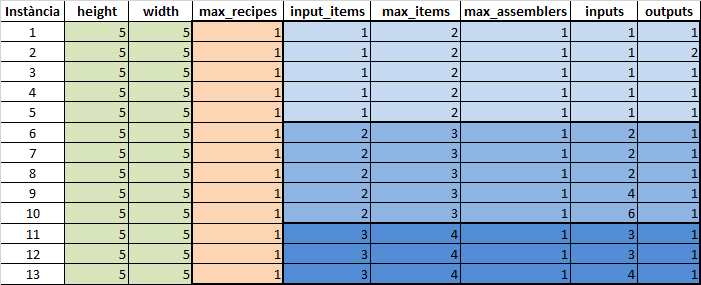
\includegraphics[width=1\linewidth]{Figures/miscelaneous/instances_5x5.png}
    \caption{Instàncies amb mida 5x5}
\end{figure}
\begin{figure}[H]
    \centering
    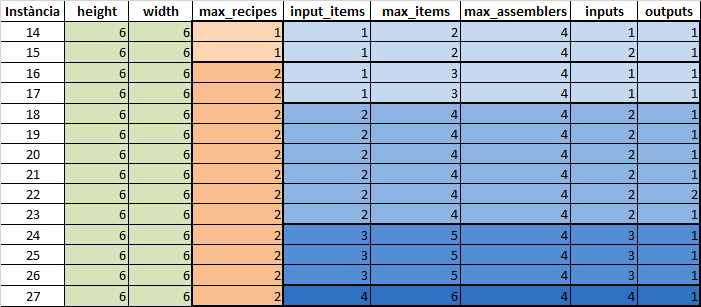
\includegraphics[width=1\linewidth]{Figures/miscelaneous/instances_6x6.png}
    \caption{Instàncies amb mida 6x6}
\end{figure}
\begin{figure}[H]
    \centering
    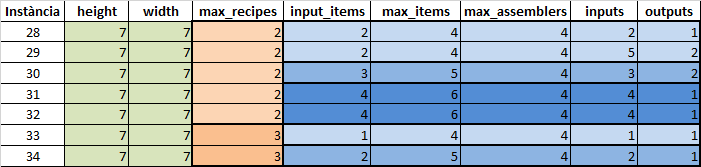
\includegraphics[width=1\linewidth]{Figures/miscelaneous/instances_7x7.png}
    \caption{Instàncies amb mida 7x7}
\end{figure}
\begin{figure}[H]
    \centering
    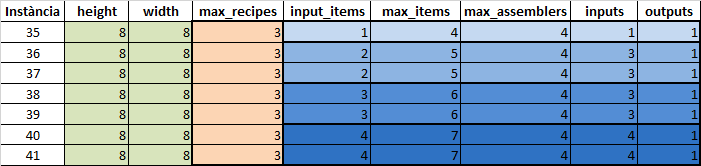
\includegraphics[width=1\linewidth]{Figures/miscelaneous/instances_8x8.png}
    \caption{Instàncies amb mida 8x8}
\end{figure}

\section{Models de proves}
Les múltiples millores que el model base ha rebut al llarg del projecte ha donat lloc a cinc versions. Aquestes s'han posat a prova resolent les instàncies anteriorment descrites, amb els tres criteris d'optimització implementats (maximització de l'objecte a fabricar, minimització de les rutes i minimització de la pèrdua d'objectes).\\
Les diferents versions del model són les següents:

\subsection{Primera versió (model base)}
Aquest model tracta de la base on s'han anat aplicant les millores i el que ha sigut descrit durant l'apartat \ref{model-base} juntament amb els canvis relacionats a les mecàniques del joc explicades a la secció \ref{mecanics-changes}. El seu rendiment és molt pobre respecte els models subseqüents, però s'ha avaluat amb la resta per poder veure la progressió que s'ha seguit al llarg del projecte.

\subsection{Segona versió (pre càlcul i bounds)}
La segona versió és la que conté les millores que més han afectat al rendiment, concretament incorpora el pre càlcul de les receptes \ref{precompute-recipes}, el lower bound respecte al nombre d'assembladors presents al blueprint \ref{lower-bound} i l'upper bound referent al domini de la variable \lstinline{route} \ref{upper-bound}

\subsection{Tercera versió (trencament de simetries 1)}
Les millores aplicades en aquest model són les del model anterior juntament amb el trencament de les simetries explicat a la secció \ref{mecanics-changes}. Tot i que a la secció mencionada només s'explica la versió final del trencament de simetries aquesta té una versió anterior molt similar que no ordena la variable auxiliar \lstinline{used}, tot i que el canvi en codi és mínim s'ha considerat usar les dues versions als experiments per veure si el canvi és gaire notori.

\subsection{Quarta versió (trencament de simetries 2)}
Aquesta versió conté el trencament de simetries amb la petita millora de l'ordenació de la variable \lstinline{used} a la implementació del trencament de la simetria.

\subsection{Cinquena versió (inseridors redundants)}
L'última versió del model incorpora l'optimització més important després del pre-calcul i els bounds, aquesta tracta de l'eliminació de la possibilitat d'usar inseridors en posicions on són redundants, afegint moltes solucions ``simètriques'' \ref{prevent-redundant-inserters}.

\section{Resultats}
Per posar a prova tots els models s'han resolt les quaranta-una instàncies usant els tres criteris d'optimització amb un time-out de trenta minuts. Les solucions a les instàncies, com s'ha explicat anteriorment, s'han descarregat i amb l'ajuda d'un script en Python, veure annex \ref{AppendixC}, s'han posat en comú tots els resultats en un fitxer Excel on s'han pogut generar tots els gràfics.\\
Els resultats s'han dividit en tres parts:
\subsection{Nombre d'instàncies resoltes}\label{subsec:instances-solved}
En aquesta secció es fa una comparativa entre les 5 versions del model i la quantitat d'instàncies que han pogut resoldre respecte a les que no s'han pogut resoldre en menys de trenta minuts. A més també es comparen aquests resultats per cada criteri d'optimització.

\begin{figure}[H]
    \centering
    \begin{subfigure}{0.4\textwidth}
        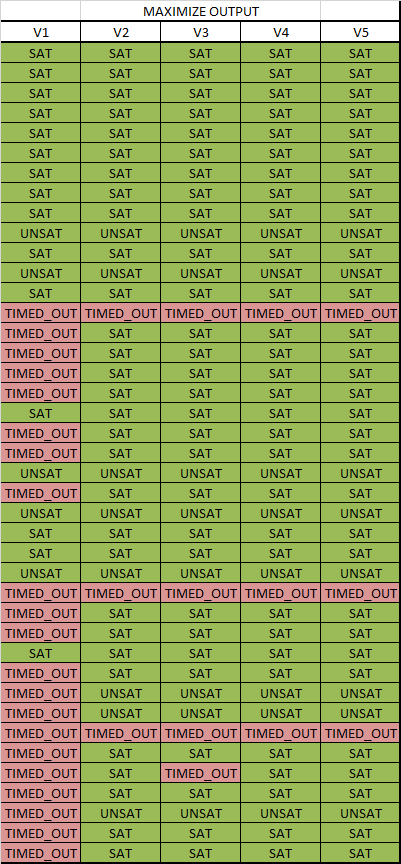
\includegraphics[width=\textwidth]{Figures/experiment_results/instances_solved_1.png}
    \end{subfigure}
    \hfill
    \begin{subfigure}{0.4\textwidth}
        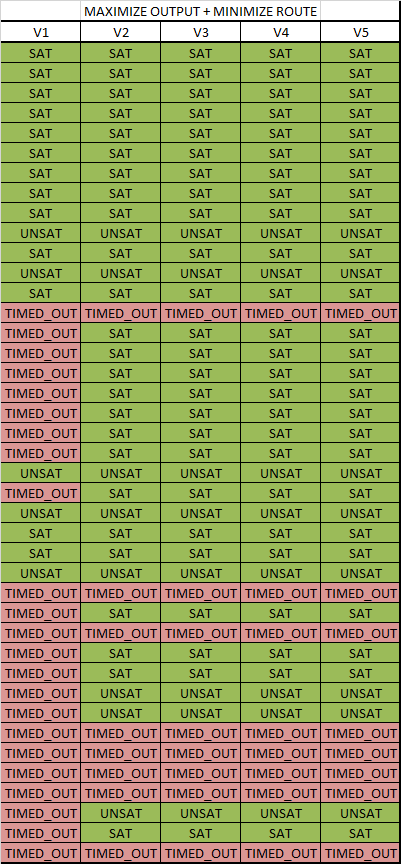
\includegraphics[width=\textwidth]{Figures/experiment_results/instances_solved_2.png}
    \end{subfigure}
    \hfill
    \begin{subfigure}{0.4\textwidth}
        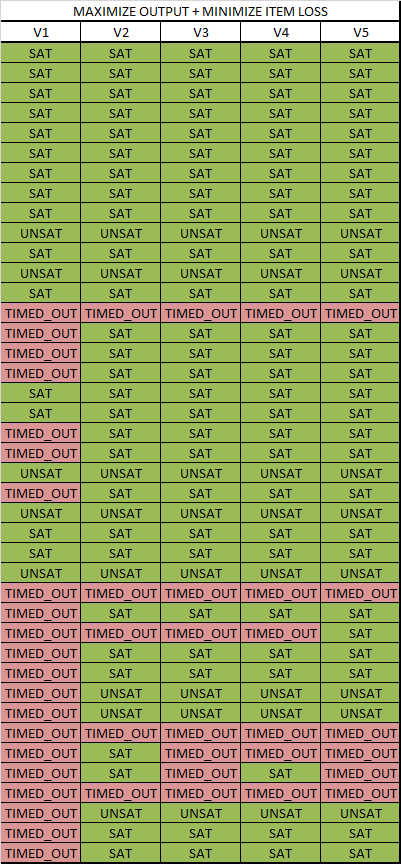
\includegraphics[width=\textwidth]{Figures/experiment_results/instances_solved_3.png}
    \end{subfigure}
    \caption{Resultat de cada instància per cada versió del model i cada criteri d'optimització}
\end{figure}

Amb aquestes taules es pot veure com la millora més dràstica és entre la primera i la segona versió del model, que és on hi ha hagut la majora de canvis importants, entre les altres versions, els canvis són mínims i en alguns casos fins i tot hi ha alguna instància que no es resol en una versió del model posterior que anteriorment si havia sigut resolta.\\
Tot seguit un recompte de les instàncies resoltes per poder veure millor el rendiment entre versions:

\begin{figure}[H]
    \centering
    \begin{subfigure}{0.6\textwidth}
        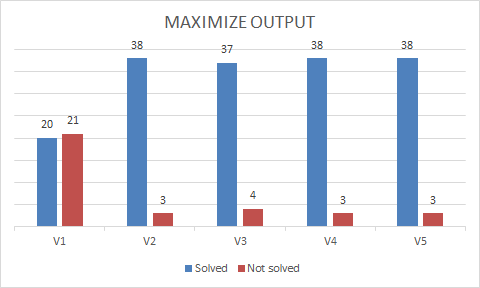
\includegraphics[width=\textwidth]{Figures/experiment_results/solved_instances_count_1.png}
    \end{subfigure}
    \hfill
    \begin{subfigure}{0.6\textwidth}
        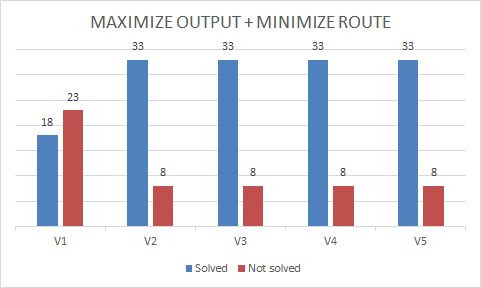
\includegraphics[width=\textwidth]{Figures/experiment_results/solved_instances_count_2.png}
    \end{subfigure}
    \hfill
    \begin{subfigure}{0.6\textwidth}
        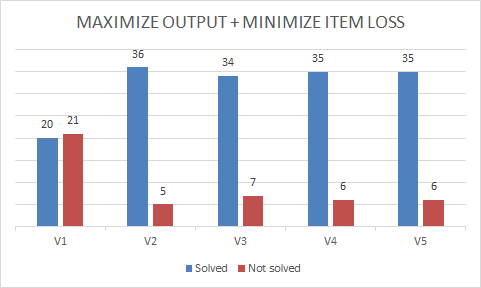
\includegraphics[width=\textwidth]{Figures/experiment_results/solved_instances_count_3.png}
    \end{subfigure}
    \caption{Nombre d'instàncies resoltes i no resoltes per versió i optimització}
\end{figure}

Amb els diagrames de barres es pot apreciar encara més el canvi entre la primera versió i les posteriors, a més també es veu com amb el criteri d'optimització que minimitza la mida de la ruta s'aconsegueixen resoldre forces menys instàncies respecte al criteri d'optimització que minimitza la pèrdua d'objectes.\\

Un detall important a mencionar és que hi ha certes instàncies que no es poden resoldre en cap de les versions, aquestes instàncies tracten concretament de la 14, 28 i 35, les quals per la mida del blueprint que tenen, el nombre de receptes que s'utilitzen i com a conseqüència el nombre d'assembladors que s'usaran és molt inferior al nombre màxim d'assembladors que hi entren. Aquesta diferència fa que el solver tingui moltes més opcions vàlides a l'hora de disposar els assembladors que es necessitaran, fent que el temps de resolució es dispari. Per aquest motiu s'ha jugat amb el nombre d'entrades del blueprint, per poder ajudar al solver reduït el nombre de possibles assignacions vàlides i reduint l'espai de solucions.

\subsection{Temps de resolució}
A continuació es mostra el temps que s'ha necessitat per resoldre cada instància per cada versió del model i criteri d'optimització juntament amb la comparació entre els temps de resolcuó de cada versió del model.

\begin{figure}[H]
    \centering
    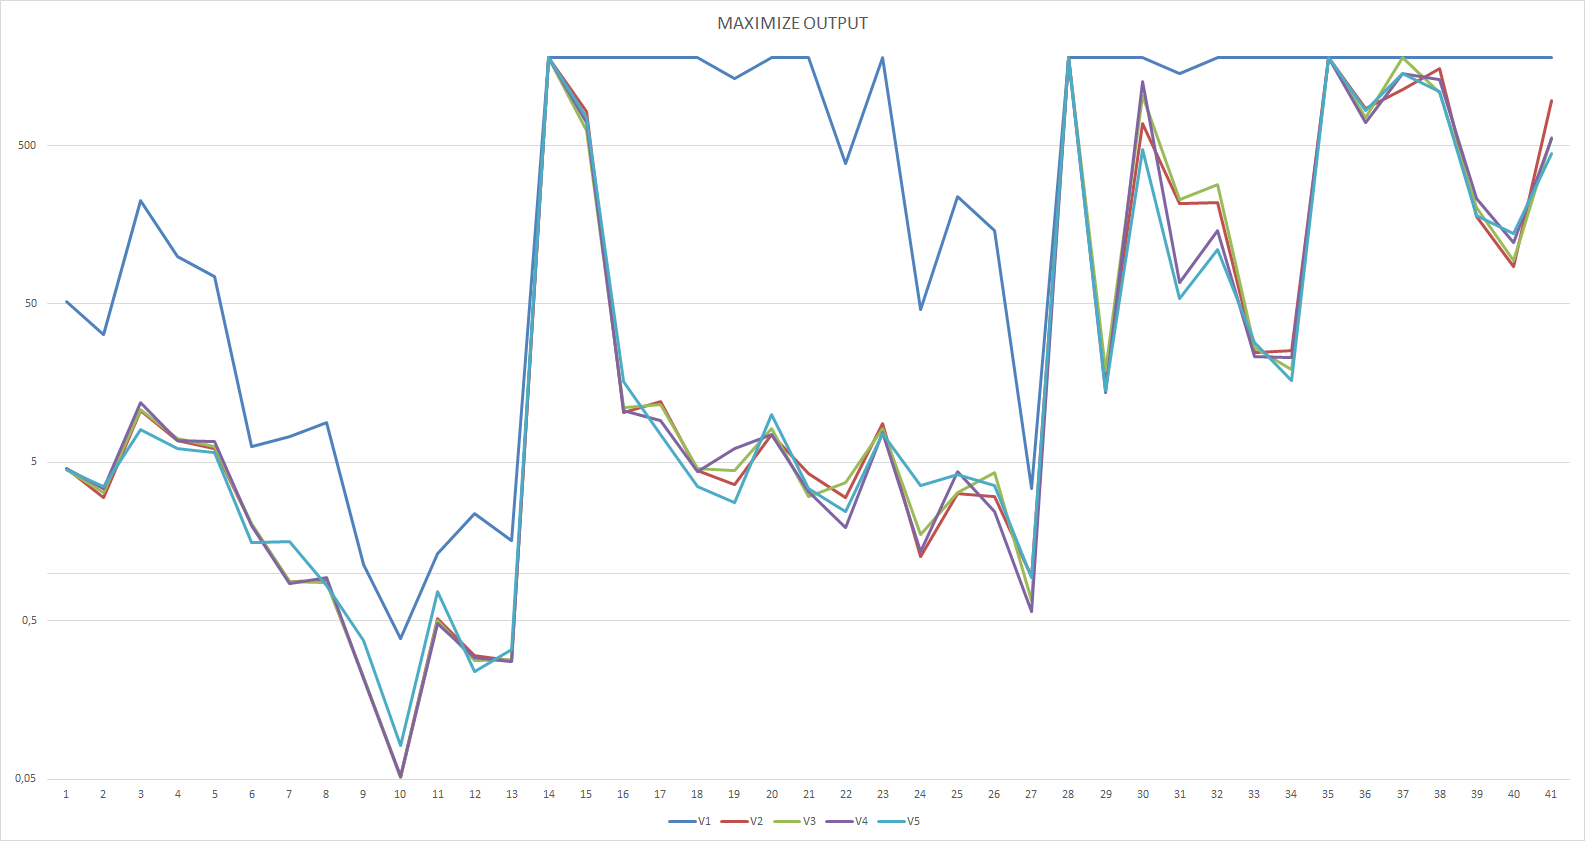
\includegraphics[width=1\linewidth]{Figures/experiment_results/solving_time_1.png}
    \caption{Comparació entre els temps de resolució dels cinc models amb el criteri d'optimització de maximitzar l'objecte objectiu}
    \label{fig:opt1_times}
\end{figure}

\begin{figure}[H]
    \centering
    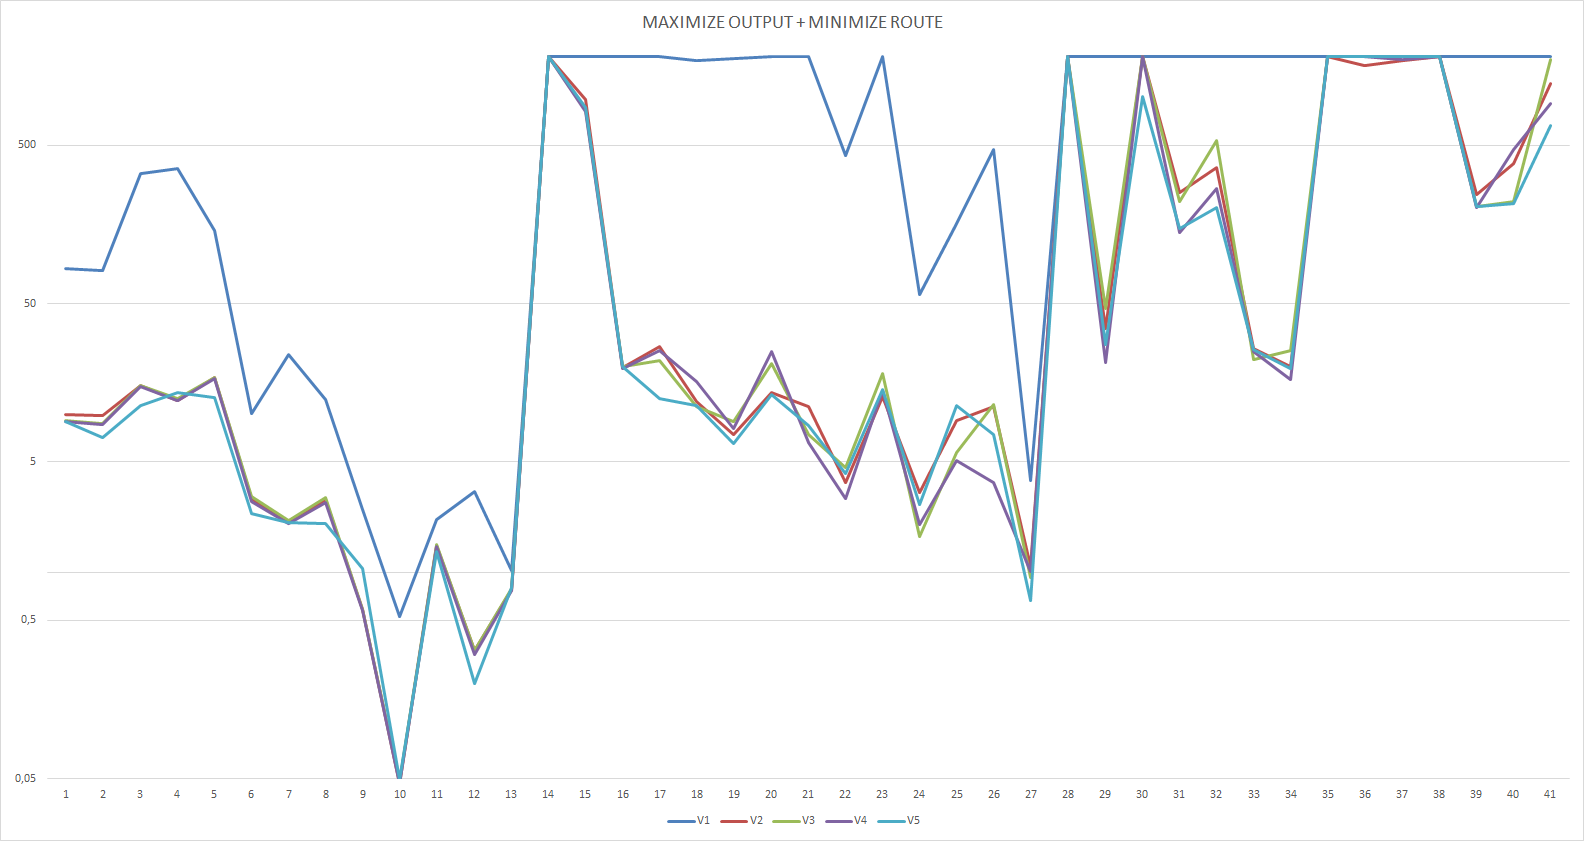
\includegraphics[width=1\linewidth]{Figures/experiment_results/solving_time_3.png}
    \caption{Comparació entre els temps de resolució dels cinc models amb el criteri d'optimització de minimitzar la mida de les rutes}
    \label{fig:opt2_times}
\end{figure}

\begin{figure}[H]
    \centering
    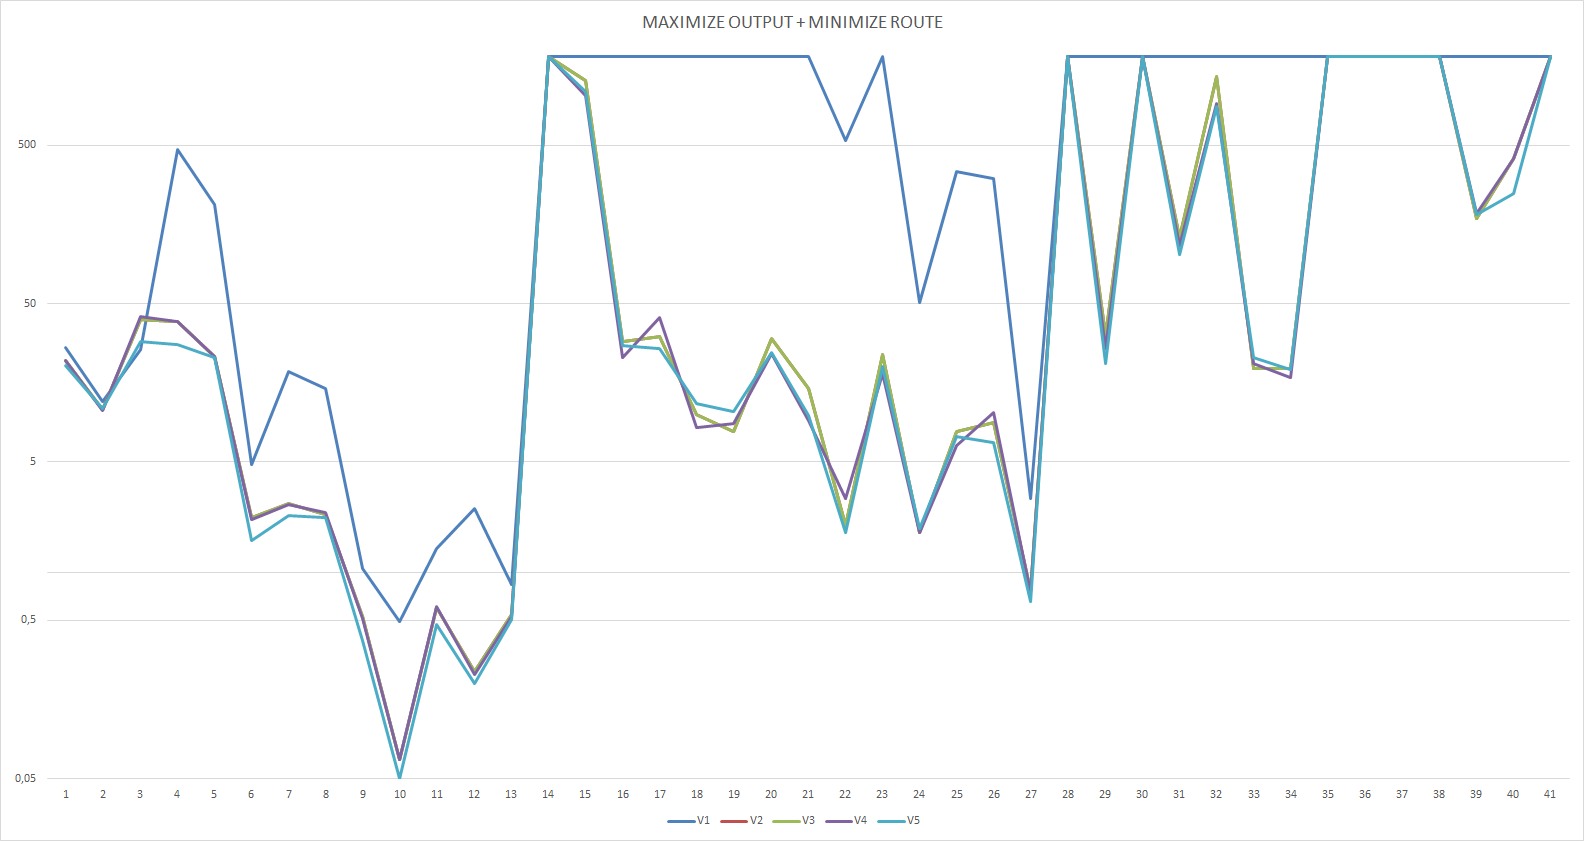
\includegraphics[width=1\linewidth]{Figures/experiment_results/solving_time_2.png}
    \caption{Comparació entre els temps de resolució dels cinc models amb el criteri d'optimització de minimitzar la pèrdua d'objectes}
    \label{fig:opt3_times}
\end{figure}

Els diagrames anteriors s'han representat en escala logarítmica a causa de la gran diferència de temps algunes d'elles, d'aquesta manera és més fàcil apreciar visualment les diferències entre les versions.\\

Si analitzem els diagrames, es poden diferenciar els quatre grups d'instàncies de mides 5x5, 6x6, 7x7 i 8x8. Ja que com s'ha explicat la mida del blueprint és un dels inputs que més repercussió té a la complexitat de la instància. Aquesta diferència es manté per tots els criteris d'optimització.\\
A banda es pot veure com al llarg de les instàncies hi ha pics i valls molt notoris, els pics són deguts principalment a les instàncies que són particularment difícils pel motiu comentat a la secció \ref{subsec:instances-solved}. Les valls d'altra banda són degudes a les instàncies que no tenen una solució satisfacible, aquestes instàncies ha resultat ser més senzilles segurament degut al fet que l'espai proporcionat envers la quantitat d'assembladors necessaris és massa poc fet sembla ajudar a propagar molt al solver fent que la solució es trobi més abans.\\
Tot i que les millores a partir de la segona versió del model pugui semblar que no són molt substancials, cal entendre que les millores aplicades és molt possible que hi hagi certes instàncies on l'optimització no sigui aplicable a causa de la falta de simetries de la instància o pocs elements de ruta usats. Això causa que certes instàncies fins i tot es pugui veure una petita pèrdua de rendiment entre versions amb més millores, ja que la complexitat afegida al model envers l'ajuda que presenten no és suficient.\\
D'altra banda instàncies que tenen moltes simetries i usen molts elements de ruta es beneficien en gran manera de les millores.\\
Per últim, als resultats es pot veure com la tercera versió del model és la que pitjor rendiment ofereix, pel fet que la implementació del trencament de simetries és massa costosa pel benefici que aporta, ja que la següent versió amb les millores aplicades al trencament de simetries hi ha múltiples instàncies que redueixen el temps de resolució múltiples minuts, donant a entendre que les solucions tenien simetries que alentien el procés de solució i que la versió anterior no les podia trencar amb la suficient eficàcia.

\subsection{Representació gràfica d'algunes instàncies resoltes}
Finalment gràcies al desenvolupament del visualitzador d'instàncies resoltes, a les figures \ref{fig:solved_example_1}, \ref{fig:solved_example_2}, \ref{fig:solved_example_3} i \ref{fig:solved_example_4} es mostren algunes de les instàncies més interessants i complexes resoltes pel model.

\begin{figure}[H]
    \centering
    \begin{subfigure}{0.45\textwidth}
        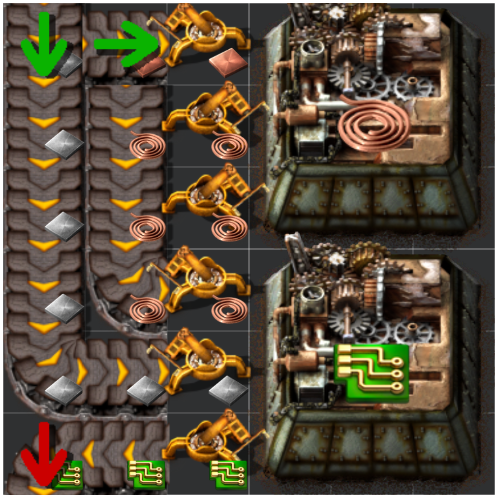
\includegraphics[width=\textwidth]{Figures/experiment_results/solved_instance_21_output.PNG}
        \caption{Maximitzar producció}
    \end{subfigure}
    \hfill
    \begin{subfigure}{0.45\textwidth}
        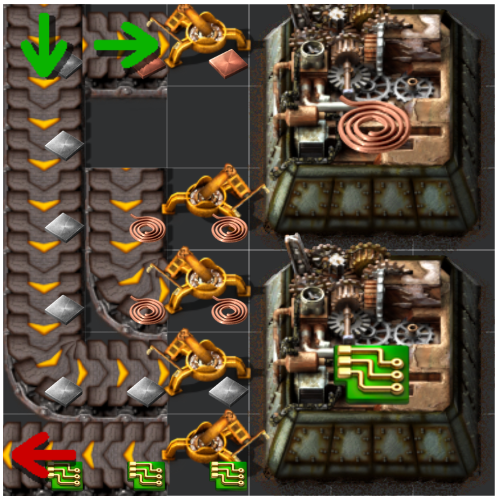
\includegraphics[width=\textwidth]{Figures/experiment_results/solved_instance_21_route.PNG}
        \caption{Minimitzar ruta}
    \end{subfigure}
    \caption{Instància amb poc espai on es pot veure com l'optimitzador de rutes només pot estalviar dos elements (cinta i inseridor)}
    \label{fig:solved_example_1}
\end{figure}

\begin{figure}[H]
    \centering
    \begin{subfigure}{0.45\textwidth}
        \includegraphics[width=\textwidth]{Figures/experiment_results/solved_instance_29_output.PNG}
        \caption{Maximitzar producció}
    \end{subfigure}
    \hfill
    \begin{subfigure}{0.45\textwidth}
        \includegraphics[width=\textwidth]{Figures/experiment_results/solved_instance_29_route.PNG}
        \caption{Minimitzar ruta}
    \end{subfigure}
    \caption{Instància on es fa ús de la unió i separació de rutes i a més el minimitzador de rutes compacta molt la solució}
    \label{fig:solved_example_2}
\end{figure}

\begin{figure}[H]
    \centering
    \begin{subfigure}{0.45\textwidth}
        \includegraphics[width=\textwidth]{Figures/experiment_results/solved_instance_39_output.PNG}
        \caption{Maximitzar producció}
    \end{subfigure}
    \hfill
    \begin{subfigure}{0.45\textwidth}
        \includegraphics[width=\textwidth]{Figures/experiment_results/solved_instance_39_route.PNG}
        \caption{Minimitzar ruta}
    \end{subfigure}
    \caption{Instància complexa on la minimització de rutes fa ús de la combinació (inseridor-cinta-inseridor) per fer arribar els objectes als assembladors}
    \label{fig:solved_example_3}
\end{figure}

\begin{figure}[H]
    \centering
    \includegraphics[width=1\linewidth]{Figures/experiment_results/solved_instance_37_output.PNG}
    \caption{Instància complexa amb dos objectes d'entrada on la producció d'un assemblador s'usa a dues receptes en diferents quantitats}
    \label{fig:solved_example_4}
\end{figure}








%----------------------------------------------------------------------------------------
% THESIS CONTENT - APPENDICES
%----------------------------------------------------------------------------------------
\appendix % Cue to tell LaTeX that the following "chapters" are Appendices

% Include the appendices of the thesis as separate files from the Appendices folder
% Uncomment the lines as you write the Appendices
% !TEX root = ../main.tex

%----------------------------------------------------------------------------------------
% APPENDIX A
%----------------------------------------------------------------------------------------

\chapter{Conversa amb el suport de Factorio} % Main appendix title

\label{AppendixA} % For referencing this appendix elsewhere, use \ref{AppendixA}
\begin{figure}[H]
    \centering
    \includegraphics[width=1\linewidth]{Figures/miscelaneous/suport_conv.png}
\end{figure}       

% !TEX root = ../main.tex

%----------------------------------------------------------------------------------------
% APPENDIX B
%----------------------------------------------------------------------------------------

\chapter{Script per compilar la informació de les instàncies} % Main appendix title
\label{AppendixB}
\begin{lstlisting}[language=Python]
    def extract_instance_data_and_write_to_excel(main_folder_path, destination_folder):
    # Initialize a dictionary to store the data
    data_output = {
        "instance": [],
        "height": [],
        "width": [],
        "max_recipes": [],
        "max_items": [],
        "max_assemblers": [],
        "input items": [],
        "input cells": [],
        "output cells": [],
        
    }
    
    # Function to sort file names based on the numerical part
    def sort_key(file_name):
        match = re.search(r'\d+', file_name)
        if match:
            return int(match.group())
        return file_name
    i = 1
    # Iterate over the JSON files
    for file in sorted(os.listdir(main_folder_path), key=sort_key):
        if file.endswith(".json"):
            file_path = os.path.join(main_folder_path, file)
            
            # Open the JSON file and extract the data
            with open(file_path, "r") as json_file:
                data = json.load(json_file)
                
                # Extract the required data
                unique_items = set()
                for recipe in data['recipes'].values():
                    for items in recipe.values():
                        for item in items:
                            unique_items.add(item[0])

                num_unique_items = len(unique_items)
                
                unique_input_items = set()
                for item in data['inOutPos']['IN'].values():
                    unique_input_items.add(item['ITEM'])
                num_unique_input_items = len(unique_input_items)
                
                num_recipes = len(data["recipes"])
                num_unique_items = len(unique_items)
                num_input_cells = len(data["inOutPos"]["IN"])
                num_output_cells = len(data["inOutPos"]["OUT"])
                height = data["size"][0]
                width = data["size"][1]
                
                # Store the data
                data_output["max_recipes"].append(num_recipes)
                data_output["max_items"].append(num_unique_items)
                data_output["input cells"].append(num_input_cells)
                data_output["output cells"].append(num_output_cells)
                data_output["input items"].append(num_unique_input_items)
                data_output["height"].append(height)
                data_output["max_assemblers"].append((width//3)*(height//3))
                data_output["width"].append(width)
                data_output["instance"].append(i)
                i+=1

    # Convert the dictionary to a DataFrame
    df = pd.DataFrame(data_output)

    # Write the DataFrame to an Excel file
    output_path = os.path.join(destination_folder, "instance_values.xlsx")
    df.to_excel(output_path, index=False)
\end{lstlisting} 
% !TEX root = ../main.tex

\chapter{Script per compilar la informació de les solucions} % Main appendix title
\label{AppendixC}
\begin{lstlisting}[language=Python]
    def extract_data_and_write_to_excel(main_folder_path, destination_folder):
    # Initialize a dictionary to store the data
    data = {
        "Iteration": [],
        "Optimization Criteria": [],
        "Status": [],
        "Solving Time": []
    }

    # Function to sort file names based on the numerical part
    def sort_key(file_name):
        match = re.search(r'\d+', file_name)
        if match:
            return int(match.group())
        return file_name

    # Iterate over the iterations
    for iteration in sorted(os.listdir(main_folder_path)):
        iteration_path = os.path.join(main_folder_path, iteration)
        
        # Iterate over the optimization criteria folders
        for criteria in sorted(os.listdir(iteration_path)):
            criteria_path = os.path.join(iteration_path, criteria)
            
            # Iterate over the JSON files
            for file in sorted(os.listdir(criteria_path), key=sort_key):
                if file.endswith(".json"):
                    file_path = os.path.join(criteria_path, file)
                    
                    # Open the JSON file and extract the data
                    with open(file_path, "r") as json_file:
                        json_data = json.load(json_file)
                        status = json_data["status"]
                        solving_time = json_data["solving_time"]
                        
                        # Store the data
                        data["Iteration"].append(iteration)
                        data["Optimization Criteria"].append(criteria)
                        data["Status"].append(status)
                        data["Solving Time"].append(solving_time)

    # Convert the dictionary to a DataFrame
    df = pd.DataFrame(data)

    # Write the DataFrame to an Excel file
    output_path = os.path.join(destination_folder, "output.xlsx")
    df.to_excel(output_path, index=False)
\end{lstlisting} 


%----------------------------------------------------------------------------------------
% BIBLIOGRAPHY
%----------------------------------------------------------------------------------------
\printbibliography[heading=bibintoc]

%----------------------------------------------------------------------------------------

\end{document}  
